\chapter{Analyse du rehaussement}

\todo{Je me rends compte que ce chapitre fait référence aux masques, mais je n'ai pas introduit les notations. J'aurais dû le faire dans le chapitre 4 Benchmark}
Nous étudions le comportement de chaque filtre sur 6 zones d'intérêts (ZI) définies par des masques binaires illustrés sur la figure FIG.~\cite{fig:areas_of_interest} :

\begin{itemize}
\item Un masque global \maskglobal, qui correspond à l'organe du volume traité. (Le foie pour le jeu de l'Ircad, le cerveau pour le jeu Bullitt et l'image entière pour le jeu VascuSynth);
\item Un masque de voisinage des vaisseaux \maskvascular, qui correspond à l'union des zones à l'intérieur des vaisseaux et des zones proches des vaisseaux (voir paragraphe de construction des zones au chapitre précédent).
\item Des masques de voisinage des vaisseaux basés sur la taille \maskvesselLarge, \maskvesselMedium, \maskvesselSmall qui produisent une partition de \maskvascular en trois zones d'intérêt en fonction du rayon des vaisseaux.
\item Un masque des bifurcations \maskbif qui se concentre sur les bifurcations à l'intérieur des vaisseaux.
\end{itemize}

\section{Conditions initiales}

Nous avons présenté dans les chapitres précédents les problématiques liées aux images médicales (Chap. 2), puis nous avons illustré les grandes familles de rehaussement de vaisseaux (Chap. 3). Nous avons ensuite construit un banc de test capable d'évaluer l'influence du rehaussement sur des zones d'intérêts précises (Chap. 4). Enfin, nous avons traité un ensemble de bases de données publiques de manière à définir 6 zones d'intérêts spécifiques.

Dans ce chapitre, nous mettons à profit l'ensemble des connaissances et outils vu précédemment afin d'analyser en détail 7 filtres de rehaussement de vaisseaux. Nous récapitulons rapidement les bases de données utilisées ainsi que les filtres sélectionnés avant de définir les métriques et la méthode d'évaluation utilisée.
\subsection{Base de données}
Nous avons à disposition trois bases de données présentées dans le Chap. 2 : L'Ircad, une base de 20 volumes en tomodensitométrie, trois versions de VascuSynth avec des niveaux de bruits Ricien différents $\sigma=\{2,4,6\}$ de 120 volumes chacune et Bullitt, une base de 33 volumes IRM en phase T2, auquel on a ajouté du bruit Ricien ($\sigma=4$) et des artefacts d'illumination. Nous disposons, pour ces jeux de données, des vérités terrains binaires des vaisseaux ainsi que d'un masque de l'organe. En plus de ce masque global, nous avons défini un masque correspondant aux vaisseaux et leur voisinage local proche. Nous avons ensuite subdivisé ce masque en 4 sous masques (3 pour Bullitt) permettant de décomposer le réseau vasculaire en partitions en fonction de la taille des vaisseaux. Enfin un dernier masque délimite la zone des bifurcations définie comme l'intérieur des embranchements des vaisseaux. Au total 6 zones d'intérêts nous permettent d'évaluer le rehaussement des vaisseaux. 

Le choix de cette évaluation par zones permet d'enrichir significativement l'analyse. En effet, le rehaussement global et le rehaussement vasculaire local peuvent être de qualité très différente. C'est par exemple le cas de filtres sensibles aux structures en plateaux comme les bordures des organes. L'évaluation par taille permet d'apporter une information supplémentaire sur les limites du rehaussement en fonction de celle-ci. Elle permet de plus de quantifier quelle partie du réseau vasculaire rehaussé participe le plus aux performances globales. Enfin, la répartition en zones permet d'évaluer les performances des filtres sur des parties peu représentatives de l'ensemble du réseau vasculaire, mais qui peuvent être critiques dans certaines applications. C'est par exemple le cas des bifurcations pour le suivis de ligne centrales.

Les 7 filtres choisis pour cette analyse sont ceux Détaillés dans le Chap. 3 et dont la construction cherche à répondre à des problématiques spécifiques différentes. Ces particularités sont résumées dans la Tab. \ref{tab:diffMethods}. 

\begin{table}[ht]
  \begin{center}
    \resizebox{\textwidth}{!}{
\begin{tabular}{l|l|l|l}
Méthode                               & Base                  &  Idée principale                              &   Date  \\ \hline  \hline 
Sato et al.      & Hessienne               & Reconnection des vaisseaux et contrôle du bruit  & 1997   \\ \hline
Frangi et al.    & Hessienne             & Contrôle du bruit ainsi que des structures en plateaux et sphériques   & 1998   \\ \hline
Meijering et al. & Hessienne             & Détection de fines structures                          & 2004 \\ \hline
OOF et al.       & Flux               & Limiter l'analyse à la surface d'une sphère pour limiter le débordement de la réponse               & 2010 \\ \hline
Jerman et al.    & Hessienne             & Augmenter l'homogénéité de la réponse et simplifier la paramétrisation            & 2016 \\ \hline
Zhang et al.     & Hessienne              & Limiter le rehaussement des bordures du foie         & 2018 \\ \hline
RORPO et al.     & Morphologie            & Discriminer les structures tubulaires par un vote de chemins orientés                         & 2018  
\end{tabular}
    }
\end{center}
\caption{Liste des filtres disponibles dans le banc de test ainsi que leur principale caractéristique.}
\label{tab:diffMethods}
\end{table}

\section{Métriques}

Pour cette expérience, nous utilisons plusieurs métriques. La majorité des métriques utilisées repose sur la comparaison voxel à voxel entre le résultat binarisé d'un filtre et un jeu de paramètres donné.

On peut classifier les voxels selon 4 classes différentes : Les vrais positifs (VP) lorsqu'il y a une correspondance 1-1 entre le $i^{ème}$ voxel du résultat binaire et le $i^{ème}$ voxel de la vérité terrain, les vrais négatifs (VN) pour une correspondance 0-0, les faux positifs (FP) lors d'une correspondance 1-0 et les faux négatifs pour une correspondance 1-0. Cette correspondance est résumée sous forme de tableau dans la table Tab: \ref{tab:confusion_matrix}.

\begin{table}
  \centering
  \begin{tabular}{ ccc }
    \hline
      & 0  & 1 \\
    0 & VN & FN \\
    1 & FP & VP  \\
    \hline
  \end{tabular}
  \caption{Matrice de confusion}
  \label{tab:confusion_matrix}
\end{table}

Des métriques définies à partir de ces quantités sont classiquement utilisées dans la littérature. Celles-ci sont définies entre 0 et 1.

\paragraph{Précision}
La précision (precision) représente la proportion de voxels prédits positifs par rapport à la proportion de voxels positifs prédits totaux.
\begin{equation}
  Précision = \frac{VP}{VP+FP}
\end{equation}

Cette mesure permet d'évaluer la proportion de voxels correctement classifiés par rapport aux voxels prédits positifs.

\paragraph{Sensibilité}

La sensibilité est le nombre de voxels positifs rééls parmi les positifs réels.

\begin{equation}
  Sensibilité = \frac{VP}{P} = \frac{VP}{VP+FN}
\end{equation}

Cette mesure permet d'évaluer si le filtre est capable de détecter tous les vaisseaux annotés par la vérité terrain ou si certains vaisseaux passent à travers la détection. 

\paragraph{Spécificité}

La spécificité est le nombre de voxels négatifs correctement prédits parmi les voxels négatifs réels.

\begin{equation}
  Spécificité = \frac{VN}{N} = \frac{VN}{VN+FP}
\end{equation}

Cette mesure permet d'évaluer si le filtre rehausse des structures non annotées dans la vérité terrain. Elle est l'équivalent pour les vrais négatifs de la sensibilité.

\paragraph{Précision (accuracy)}

La précision (accuracy), est une métrique plus large que la précision. Elle prend en compte le classement correct des voxels positifs et négatifs. 

\begin{equation}
  Précision_{acc} = \frac{VP+VN}{P+N} = \frac{VP+VN}{VP+VN+FP+FN}
\end{equation}

La précision mesure la qualité de la classification globale, à la fois le bon rehaussement et à la fois l'absence de faux rehaussement.

Bien que toutes ces mesures soient informatives d'un aspect particulier de la segmentation, elles n'ont pas toutes le même poid. En effet, les vaisseaux représentent moins de 5 pourcents de l'ensemble des voxels d'un volume. Le poids des voxels négatifs peut donc dans certaines mesures submerger le poid des voxels positifs, on peut ainsi être amené à sous estimer des erreurs en utilisant par exempel la Précision (accuracy). Parmis ces mesures, les plus significatives pour notre étude sont la sensibilité et la précision (precision).


\paragraph{Dice}

Le Dice, aussi connu sous le nom de F1-score est une mesure de recouvrement entre le volume binaire de la vérité terrain et le volume binaire prédit. Il s'exprime comme l'intersection sur union de la vérité terrain et du volume binaire prédit.

\begin{equation}
  \textrm{Dice} = \frac{2 \textrm{VP}}{\textrm{FP} + \textrm{FN} + 2 \textrm{VP}} \\ 
\end{equation}

Le Dice est une mesure populaire dans la littérature, mais il n'exprime que le recouvrement des voxels positifs correctement classifiés. Un recouvrement total aura une mesure de 1 là où un recouvrement nul aura une mesure de 0. Cette mesure ne différencie pas deux volumes binaires dont la forme serait très différente à partir du moment où l'intersection entre les deux volumes et la vérité terrain serait la même. Dans notre analyse, le Dice sert de mesure d'évaluation secondaire. Il permet notamment d'évaluer les performances du rehaussement des bifurcations, puisque la métrique principale n'est pas définit dans cette zone d'intérêt.

\paragraph{Coefficients de corrélation de Matthew}

Les coefficients de corrélation de Matthew (MCC), un cas spécifique du score $\phi$, est plus  expressif que le Dice puisqu'il intègre la classification correcte du fond, les vrais négatifs, dans la mesure. Cette métrique est définie entre -1 et 1 avec 1 un volume binaire égal à la vérité terrain et -1 un volume binaire étant le complémentaire de la vérité terrain.

\begin{equation}
  \textrm{MCC} = \frac{\textrm{tp} \cdot \textrm{tn} - \textrm{fp} \cdot \textrm{fn}}{\sqrt{(\textrm{tp}+\textrm{fp})(\textrm{tp}+\textrm{fn})(\textrm{tn}+\textrm{fp})(\textrm{tn}+\textrm{fn})}}
\end{equation}

Bien que le Dice est plus commun dans la littérature, le MCC est présenté par Chicco et Jurman \cite{Chicco2020_advantages_MCC_Dice} comme une mesure plus stable pour les structures éparses tel que les vaisseaux. Le MCC n'est pas défini dans un certains nombres de cas, et notamment lorsque les zones d'intérêts sur lesquels sont caculés les métriques ne contiennent pas de voxels négatifs. Pour ces zones, on utilise le Dice pour l'évaluation. 


\paragraph{Rapport signal sur bruit}

%\todo{ Est-ce que je garde le SNR sachant qu'au final on ne l'a jamais exploité ?}

Nous avons souhaité intégrer une mesure au banc de test qui ne dépend pas d'un processus de binarisation, mais exprime la distance entre la vérité terrain et la sortie du filtre.

Le PSRN est habituellement utilisés pour évaluer le degré de dégradation d'une image causé par un bruit. C'est par exemple le cas d'un message qui subirait des pertes lorsque que celui-ci est envoyé à travers un canal de communication. Il est défini par :

\begin{align}%\label{Eq: SNR_and_PSNR}
  %\nonumber
  %\textrm{SNR} & = \log_{10}\Big( \frac{1}{|I|}\frac{ \sum_{x} I_{\textrm{Filter}}(x)^2 }{ \sum_{x} I_{\textrm{Ground-truth}}(x)^2 } \Big) \\
 \nonumber
  \textrm{PSNR} & = \log_{10}\Big( \frac{ (\max_x I(x))^2  }{ \textrm{MSE}( I_{\textrm{GT}}, I_{\textrm{Filter}} ) } \Big)
\end{align}

Avec $I$ l'image de sortie normalisée, $I_{filter}$ l'image filtrée, $I_{GT}$ l'image binaire normalisée et MSE l'erreur au sens des moindres carrés. Plus le PSNR est haut, plus l'image filtrée est proche de l'image binarisée. Dans le cas où les deux sont égales, le PSNR est infini.

Dans notre cas, nous utilisons le PSNR comme une mesure de similarité entre la sortie du filtre non binarisée et la vérité terrain normalisée (0 ou 1). Afin que des comparaisons fiables puissent être effectuées entre deux sorties de filtres, il est nécessaire de faire une mise à l'échelle de l'intensité de sortie du filtre entre 0 et 1 et de la vérité terrain (1 et non 255). En effet, nous nous sommes assuré que tous les filtres aient une sortie définie entre 0 et 1 (Chap. 4) mais rien ne garanti que la plage de rehaussement couvre l'ensemble de l'intervalle [0,1] et non un intervalle quelconque comme [0,0.3]. Il n'y a en effet pas de raisons, autre que pour des considérations de visualisation par l'œil humain, de différencier deux filtres (ou jeux de paramètres) produisant le même résultat binaire après seuillage, mais dont la dynamique est définie sur deux plages différentes.

Un faible PSNR nous indique soit que le rehaussement est très bruité ou alors que le niveau général de l'intensité du rehaussement est faible.


\paragraph{Courbe ROC}

La courbe ROC (Receiving operator caracteristic) est une visualisation de l'évolution du taux de vrai positif en fonction du taux de faux positif au fur et à mesure des seuillages successifs appliqués au filtre. Le taux de vrai positif correspond à la sensibilité et le taux de faux positif est égal à $1-\text{spécificité}$. 

Cette courbe donne une vue globale différente sur les performances des filtres. Nous avons évalué les autres métriques comme une mesure des meilleures performances d'un filtre et d'un jeu de paramètre. Elle nous permet d'évaluer asymptotiquement les performances entre deux filtres à travers de multiples seuils.

Lors de la construction de courbes ROC, il faut éviter quelques pièges. Une courbe ROC classique est définie par un ensemble de points $P$ qui forment un pseudo arc de cercle entre les points (0,0) et (1,1). Dans le cas des filtres de rehaussement, la répartition des points sur l'arc est très hétérogène. Cette hétérogénéité dépend souvent de la diversité géométrique des structures rehaussées, car deux structures qui possèdent la même géométrie auront une valeur de rehaussement similaire, alors que des structures différentes seront détectées à des seuils de tubularité différents. Ce point devient problématique lorsque l'on veut effectuer une courbe ROC moyenne pour un filtre et un jeu de paramètre donné appliqué à l'ensemble des volumes d'une phrase. Par exemple, si l'on a 3 courbes ROC de 200 points chacune représenté sous la forme d'une liste de points, on ne peut pas moyenner les points en fonction des indices ( $m_i = (ROC^1_{i} + ROC^2_{i} + ROC^3_{i}/3 $). Les points ne sont en effet pas échantillonés de la même manière sur la courbe et la moyenne est faussée (Fig. \ref{fig:good_and_bad_roc}). Pour échapper à ce problème, il est nécessaire d'interpoler chaque courbe de manière à obtenir le même échantillonage régulier sur chaque courbe. On obtient ainsi une courbe réellement représentative de la moyenne des ROC.


\begin{figure}[ht]
  \centering
  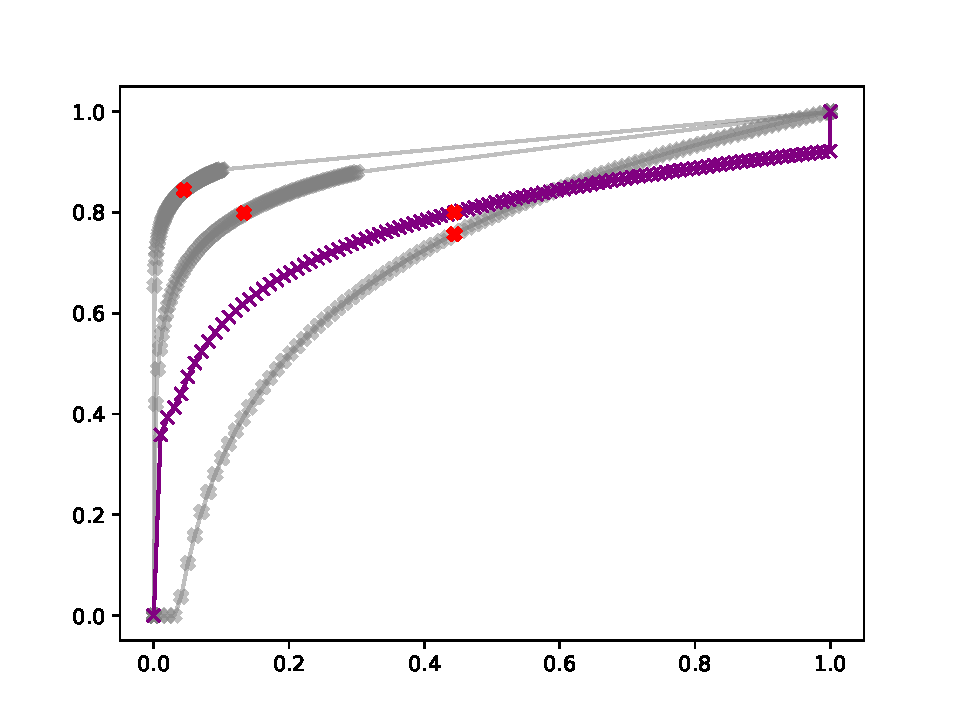
\includegraphics[height=4cm]{Images/ROC_badMean.pdf}
  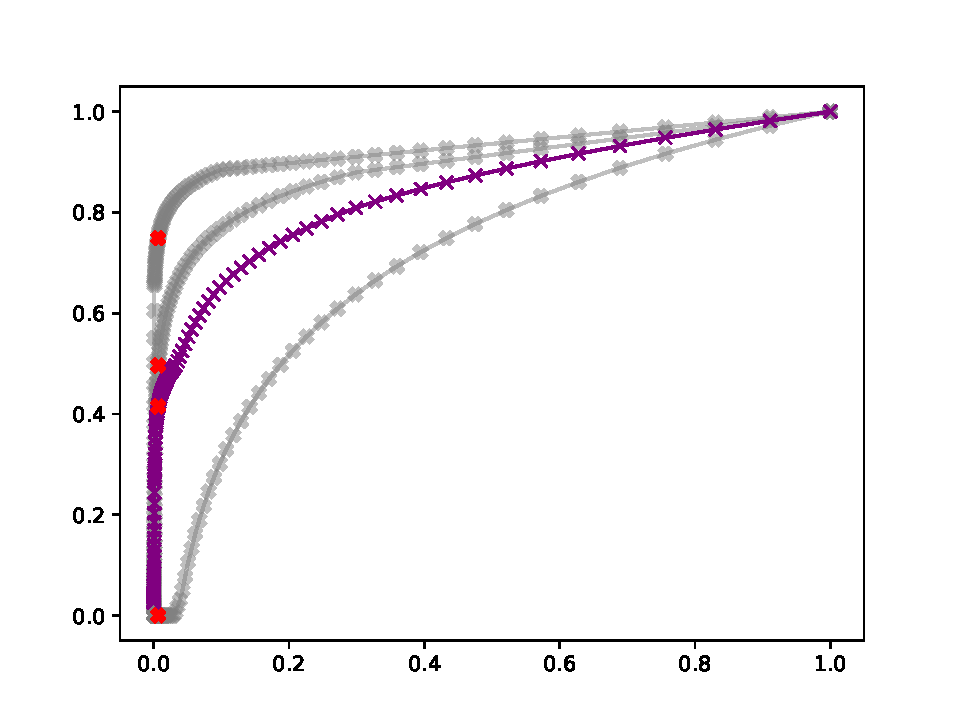
\includegraphics[height=4cm]{Images/ROC_goodMean.pdf}
  \caption{En violet courbe ROC moyenne construite à partir des courbes ROC en gris. À gauche, la courbe moyenne est construite sans interpolation. À droite, courbe ROC avec interpolation.}
  \label{fig:good_and_bad_roc}
\end{figure}

\section{Optimisation}

Nous avons cherché à comprendre si une paramétrisation idéale des filtres était possible et sinon quels étaient les règles régissants le choix des paramètres. En effet ces choix sont expliqués théoriquement, mais la manière de les régler est rarement décrite. À la place, des paramètres par défaut sont proposés. C'est par exemple le cas de Frangi ($\alpha=0.5,\beta=0.5$), ou Sato $(\alpha_1=0.5,\alpha_2=2$) dont les recommandations sont reprises dans de nombreux articles. Ces paramètres sont rarement discutés. Pourtant, dans certains articles plus applicatifs, les paramètres utilisés par les auteurs sont différents. Par exemple, Marcan et al. \cite{Marcan2014_vessel_seg} pour la segmentation dans l'IRM du foie propose d'utiliser ($\alpha=0.3,\beta=0.7$) dans sa chaine de segmentation. On peut donc légitimement se demander quel est l'impact des paramètres sur le rehaussement final et quels paramètres utiliser en fonction d'une base de donnée spécifique.

Pour répondre à cette question, nous avons cherché à optimiser les filtres de manière à proposer un rehaussement optimal pour une segmentation la plus élémentaire possible. L'objectif était ainsi de pouvoir analyser le rehaussement au plus prêt des filtres sans parasitage provoqué par du prétraitement ou du post traitement.

Nous avons choisi de définir l'optimalité du rehaussement par rapport au MCC mesuré entre la vérité terrain binaire des vaisseaux et des volumes filtrés puis binarisés. En effet, le MCC permet à la fois de mesurer la qualité du rehaussement des vaisseaux, mais elle permet aussi de hiérarchiser plus précisément le rehaussement de structures erronées, contrairement au Dice qui n'intègre pas les voxels négatifs dans sa mesure. L'optimalité d'une métrique dépend aussi de la zone d'intérêt sélectionnée pour effectuer l'optimisation. Pour cela, nous avons choisi le masque \maskglobal afin de prendre en compte l'ensemble des problématiques du rehaussement : la détection des vaisseaux, la  différenciation avec les autres structures, la qualité du filtrage et l'amélioration du signal des vaisseaux. 

Nous aurions également pu choisir de maximiser le rehaussement des vaisseaux en utilisant le voisinage des vaisseaux comme zone d'optimisation. On aurait ainsi trouvé les paramètres permettant un rehaussement des vaisseaux avec la plus grande qualité. Cependant, pour des considérations de temps, de puissance de calcul et de volume de données à analyser, nous avons choisis de n'optimiser les paramètres que par rapport à une seule zone d'intérêt.

L'ensemble des paramètres liés aux filtres de rehaussement peuvent être classifiés en deux groupes : Les paramètres d'échelles qui définissent la fenêtre permettant de capturer la taille des vaisseaux et Les paramètres intrinsèques des méthodes permettant de détecter la forme des vaisseaux. Par exemple, le filtre de Frangi possède 3 paramètres liés à l'échelle et trois paramètres qui pondèrent la réponse en fonction de la géométrie. Quand un nombre élevé de paramètres $K >> 1$ nécessite d'être optimisé (e.g. $k=6$ pour Frangi), trouver un jeu de paramètres optimal induit par l'espace à k-dimensions est coûteux en temps de calcul.

Dans nos expériences, nous avons choisis d'optimiser l'ensemble des paramètres en deux étapes :

\begin{itemize}
\item L'optimisation de l'échelle en utilisant des paramètres intrinsèques fixes.
\item L'optimisation des paramètres intrinsèques en utilisant le jeu d'échelles optimales trouvé à l'étape précédente.
\end{itemize}

Les paramètres intrinsèques fixes sont ceux recommandés par les auteurs des méthodes ou sont choisis empiriquement.  Pour chaque étape, les paramètres optimaux sont définis au sens du meilleur MCC moyen dans le masque global (\maskglobal) du jeu de données entier. Cette stratégie en deux étapes peut être comparée à un choix naturel où un utilisateur commence dans un premier temps par choisir les paramètres d'échelles en se basant sur des observations des structures biologiques avant de raffiner le rehaussement (Fig. \ref{fig:flowchart_opti}).

\begin{figure}[!ht]
  \centering
  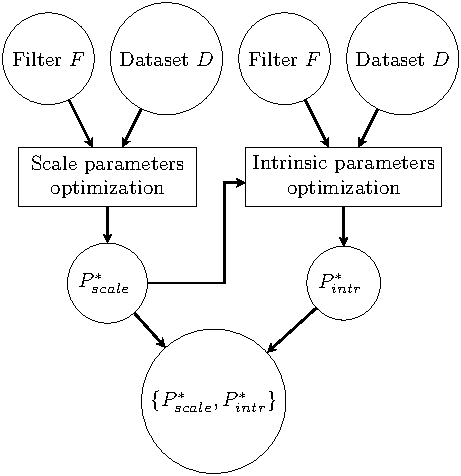
\includegraphics[height=6cm]{Images/flowchart_benchmark.pdf}
  \caption{Diagramme illustrant l'optimisation en deux temps. D'abords l'optimisation de l'échelle puis l'optimisation des paramètres intrinsèques.}
  \label{fig:flowchart_opti}
\end{figure}


\subsection{Méthode de calcul}
\subsubsection{calcul du MCC moyen}
  Le calcul du MCC moyen a subi deux itérations dans la manière de procéder.  On considère pour la suite de cette section que tous les calculs sont réalisés dans un seul masque par soucis de clarté. De la même manière, on considère un seul filtre $F$ ainsi qu'un seul jeu de données $D$.

  \paragraph{Première itération}
  Pour chaque volume $v_i \in D$, on calcule la réponse du filtre $F$ avec le jeu de paramètre $P_j$ afin d'obtenir le volume filtré $R = F_{P_j}(v_i)$. Pour un nombre $S$ de seuils choisi par l'utilisateur, on binarise le volume $S$ fois puis l'on calcule le MCC pour chaque seuil ($MCC_{F_{P_j},v_i,s_k}$).
  
  Puis, pour chaque $P_{j,F}$ on calcule un MCC moyen par seuil $\overline{MCC}_{ P_{j,F} } =  \frac{1}{N} \sum_{N}^i MCC_{F_{P_j},v_i,s_k}$. On assigne ensuite à chaque paramètre le MCC moyen maximum. Le jeu de paramètres optimal $P*$ est alors le jeu avec le MCC moyen maximal :
  
  \begin{equation}
    P* =  argmax_ {P_j \in P}( \overline{MCC}_{ F_{P_j} } )
  \end{equation}

  Cette méthode, utilisée dans nos premier travaux (ICPR), souffre des mêmes limitations qu'une moyenne effectuée naïvement pour calculer des courbes ROC. Elle moyenne en effet des rehaussements ayant des dynamiques différentes, ce qui sous estime les résultats. La démarche initiale de cette méthode était d'émuler un fonctionnement où un opérateur aurait à manipuler un algorithme de segmentation paramétré une seule fois pour une utilisation régulière.
  
  \paragraph{Deuxième itération}
  Pour la deuxième itération, il a été choisi de maximiser le MCC du rehaussement dès l'étape de seuillage en choisissant le seuil maximisant le MCC, plutôt que de moyenner le MCC par seuil. Ainsi, $MCC_{F_{P_j},v_i} = max_{s_k \in S} ( MCC_{F_{P_j},v_i,s_k} ) $ et  $\overline{MCC}_{ P_{j,F} } =  \frac{1}{N} \sum_{N}^i MCC_{F_{P_j},v_i} $. On obtient ainsi la moyenne du meilleur MCC par volume. Le jeu de paramètres optimal $P*$ est alors le jeu avec le MCC moyen maximal :
  
  \begin{equation}
    P* =  argmax_ {P_j \in P}( \overline{MCC}_{ F_{P_j} } )
  \end{equation}


  Dans cette itération, on émule un fonctionnement où un opérateur est capable de paramétrer pour chaque volume le seuil idéal. On tire donc le maximum des performances du pipeline de segmentation. Cette manière de procéder est utilisée aux deux étapes de l'optimisation sans changement de l'algorithme. Dans notre analyse, le pas entre chaque seuil de 0.005 est appliqué, ce qui résulte en 201 seuils binaires.

  \subsubsection{Choix des paramètres}

Une stratégie de recherche exhaustive (grid search) est réalisée pour ces paramètres. Les conditions de cette recherche sont résumés dans la table Tab. \ref{tab:SS_interval}, Tab. \ref{tab:SS_interval_RORPO} (paramètres d'échelles) et TABLE \ref{table:PS_interval} (paramètres intrinsèques).

Le choix des paramètres a été fait de manière à effectuer un compromis entre temps de calcul total du banc de test, espacement des paramètres et exhaustivité. Les limites des paramètres d'échelles ont été définies à la main en mesurant la taille des structures sur des images isotropes de $[1mm,1mm,1mm]$ de résolution des troncs des réseaux vasculaires pour la limite haute et les limites de la résolution d'un pixel pour la limite basse. En effet, une gaussienne de taille inférieure à un pixel n'a pas de sens. De même, tous jeux de paramètres d'échelle dont la différence entre chaque échelle une à une est inférieure à $\frac{1}{6}$ est éliminée. Pour RORPO, un delta minimal entre deux tailles de chemins est aussi défini de manière empirique.

\begin{table}[H]
  \caption{Paramètres d'échelles pour les filtres utilisant un espace d'échelles basé sur le diamètre :  Frangi, Sato, Meijering, Jerman, Zhang, OOF (recherche par grille information). Les conditions  assurent que l'écart entre chaque échelle $i$ est supérieur à la résolution d'un voxel.}
  \label{tab:SS_interval}
  \begin{center}
    \begin{tabular}{  l  c  c  c }
      \hline
      \multicolumn{4}{c}{ Ircad et VascuSynth }\\
      \hline
      Pramètres & Intervalle & Pas & Conditions \\
      \hline
      $\sigma_{\min}$ & $[0.4,1.8]$ & $0.4$ & \\
      $\sigma_{\max}$ & $[1.4,3.4]$  & $0.4$ & $\sigma_{min,i} - \sigma_{max,i} > \frac{1}{6}$ mm \\ 
      Nombre d'échelles & $[\![3,4]\!]$ & $1$ & \\
      \hline
      \hline
      \multicolumn{4}{c}{ Bullitt }\\
      \hline
      Paramètres & Intervalle & Pas & Conditions \\
      \hline
      $\sigma_{\min}$ & $[0.2,1.6]$ & $0.4$ & \\
      $\sigma_{\max}$ & $[1.2,3.2]$  & $0.4$ & $\sigma_{min,i} - \sigma_{max,i} > \frac{1}{6}$ mm \\ 
      Nombre d'échelles & $[\![3,4]\!]$ & $1$ & \\
      \hline
    \end{tabular}
  \end{center}
\end{table}

\begin{table}[H]
  \caption{ Paramètres d'échelles pour RORPO sans le paramètre de dilatation (recherche en grille). Les conditions d'espacement entre chaque échelle $i$ assure que deux échelles successives ne soient pas trop similaires.}
  \label{tab:SS_interval_RORPO}
  \begin{center}
    \begin{tabular}{  l  c  c  c }
      \hline
      \multicolumn{4}{c}{Ircad}\\
      \hline
      Paramètres & Intervalle & Pas & Conditions \\
      \hline
      Échelle min. & $[30,150]$ & $10$ & \\
      Facteur & $[1.1,1.6]$ & $0.1$ & $20 < \textrm{scale}_{i} - \textrm{scale}_{j} < 200$ \\ 
      Nb. d'échelles & $[\![2,4]\!]$ & $1$ & \\
      \hline
      \hline
      \multicolumn{4}{c}{Bullitt}\\
      \hline
      Paramètres & Intervalle & Pas & Conditions \\
      \hline
      Échelle min. & $[30,90]$ & $10$ & \\
      
      Factor & $[1.1,1.5]$  & $0.1$ & $ 20 < \textrm{scale}_{i} - \textrm{scale}_{j} < 200$ \\
      Nb. scales & $[\![2,4]\!]$ & $1$ & \\
      \hline
      \hline
      \multicolumn{4}{c}{VascuSynth}\\
      \hline
      Paramètres & Intervalle & Pas & Conditions \\
      \hline
      Échelle min. & $[10,90]$ & $10$ & \\
      
      Facteur & $[1.1,1.5]$  &  $0.1$ & $ 9 < \textrm{scale}_{i} - \textrm{scale}_{j} < 100$ \\
      
      Nb. d'échelles & $[\![2,4]\!]$ & $1$ & \\
      \hline
    \end{tabular}
  \end{center}
\end{table}

\begin{table}[H]
  \caption{Paramètres intrinsèques (recherche par grille). Meijering et RORPO n'ont pas de paramètres intrinsèques.}
  \label{table:PS_interval}
  \begin{center}
    \begin{tabular}{  l  c  c  c }
      \hline
      Filtres & Paramètres & Intervalle & Pas \\
      \hline
      Frangi & $\alpha$ & $[0.2,1.0]$ & $0.2$ \\
      ---       & $\beta$ & $[0.2,1.0]$ & $0.2$  \\
      ---       & $C$& $[0,60]$ & $30$ \\
      Sato & $\alpha_{1}$ & $[0.2,1.0]$ & $0.2$ \\
      ---     & $\alpha_{2}$ & $[1,2]$ & $0.2$ \\
      OOF & $\sigma$ & $[0.1,1.0]$ & $0.1$ \\
      Jerman & $\tau$ & $[0.1,1.0]$ & $0.1$ \\
      Zhang & $\tau$& $[0.1,1.0]$ & $0.1$ \\
      \hline
    \end{tabular}
  \end{center}
\end{table}
  
Au total, 41 jeux de paramètres d'échelles sont testé pour les filtres Hessiens et OOF. Respectivement 32, 44 et 51 jeux de paramètres sont testé pour RORPO sur l'Ircad, VascuSynth et Bullitt. Pour les paramètres intrinsèques, 10 jeux de paramètres sont testés pour Jerman,Zhang et OOF. 75 jeux de paramètres sont testés pour Frangi et 30 pour Sato.


\section{Résultats}

Dans cette section, nous présentons et discutons les résultats quantitatifs et qualitatifs des différents filtres. En plus des sept filtres présentés précédemment, nous ajoutons un simple seuillage comme référence. La sortie de cette référence est l'image d'entrée normalisée et seuillée de manière à ce le seuil soit optimisé de la même manière que les autres paramètres.

Dans la suite, on commence par analyser les résultats des filtres dans le masque global \maskglobal. Ensuite, nous discutons des résultats obtenus sur les masques vasculaires \maskvascular, \maskvesselLarge, \maskvesselMedium, \maskvesselSmall. Enfin, nous exposons les résultats obtenus au niveau des bifurcations.

\subsection{Résultats globaux}

\begin{figure}[!ht]
  \centering
  \begin{subfigure}[t]{0.4\textwidth}
    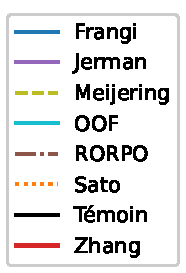
\includegraphics[clip = true, height=43mm]{Images/standAloneLegend.pdf}
  \end{subfigure}
  \begin{subfigure}[t]{0.4\textwidth}
  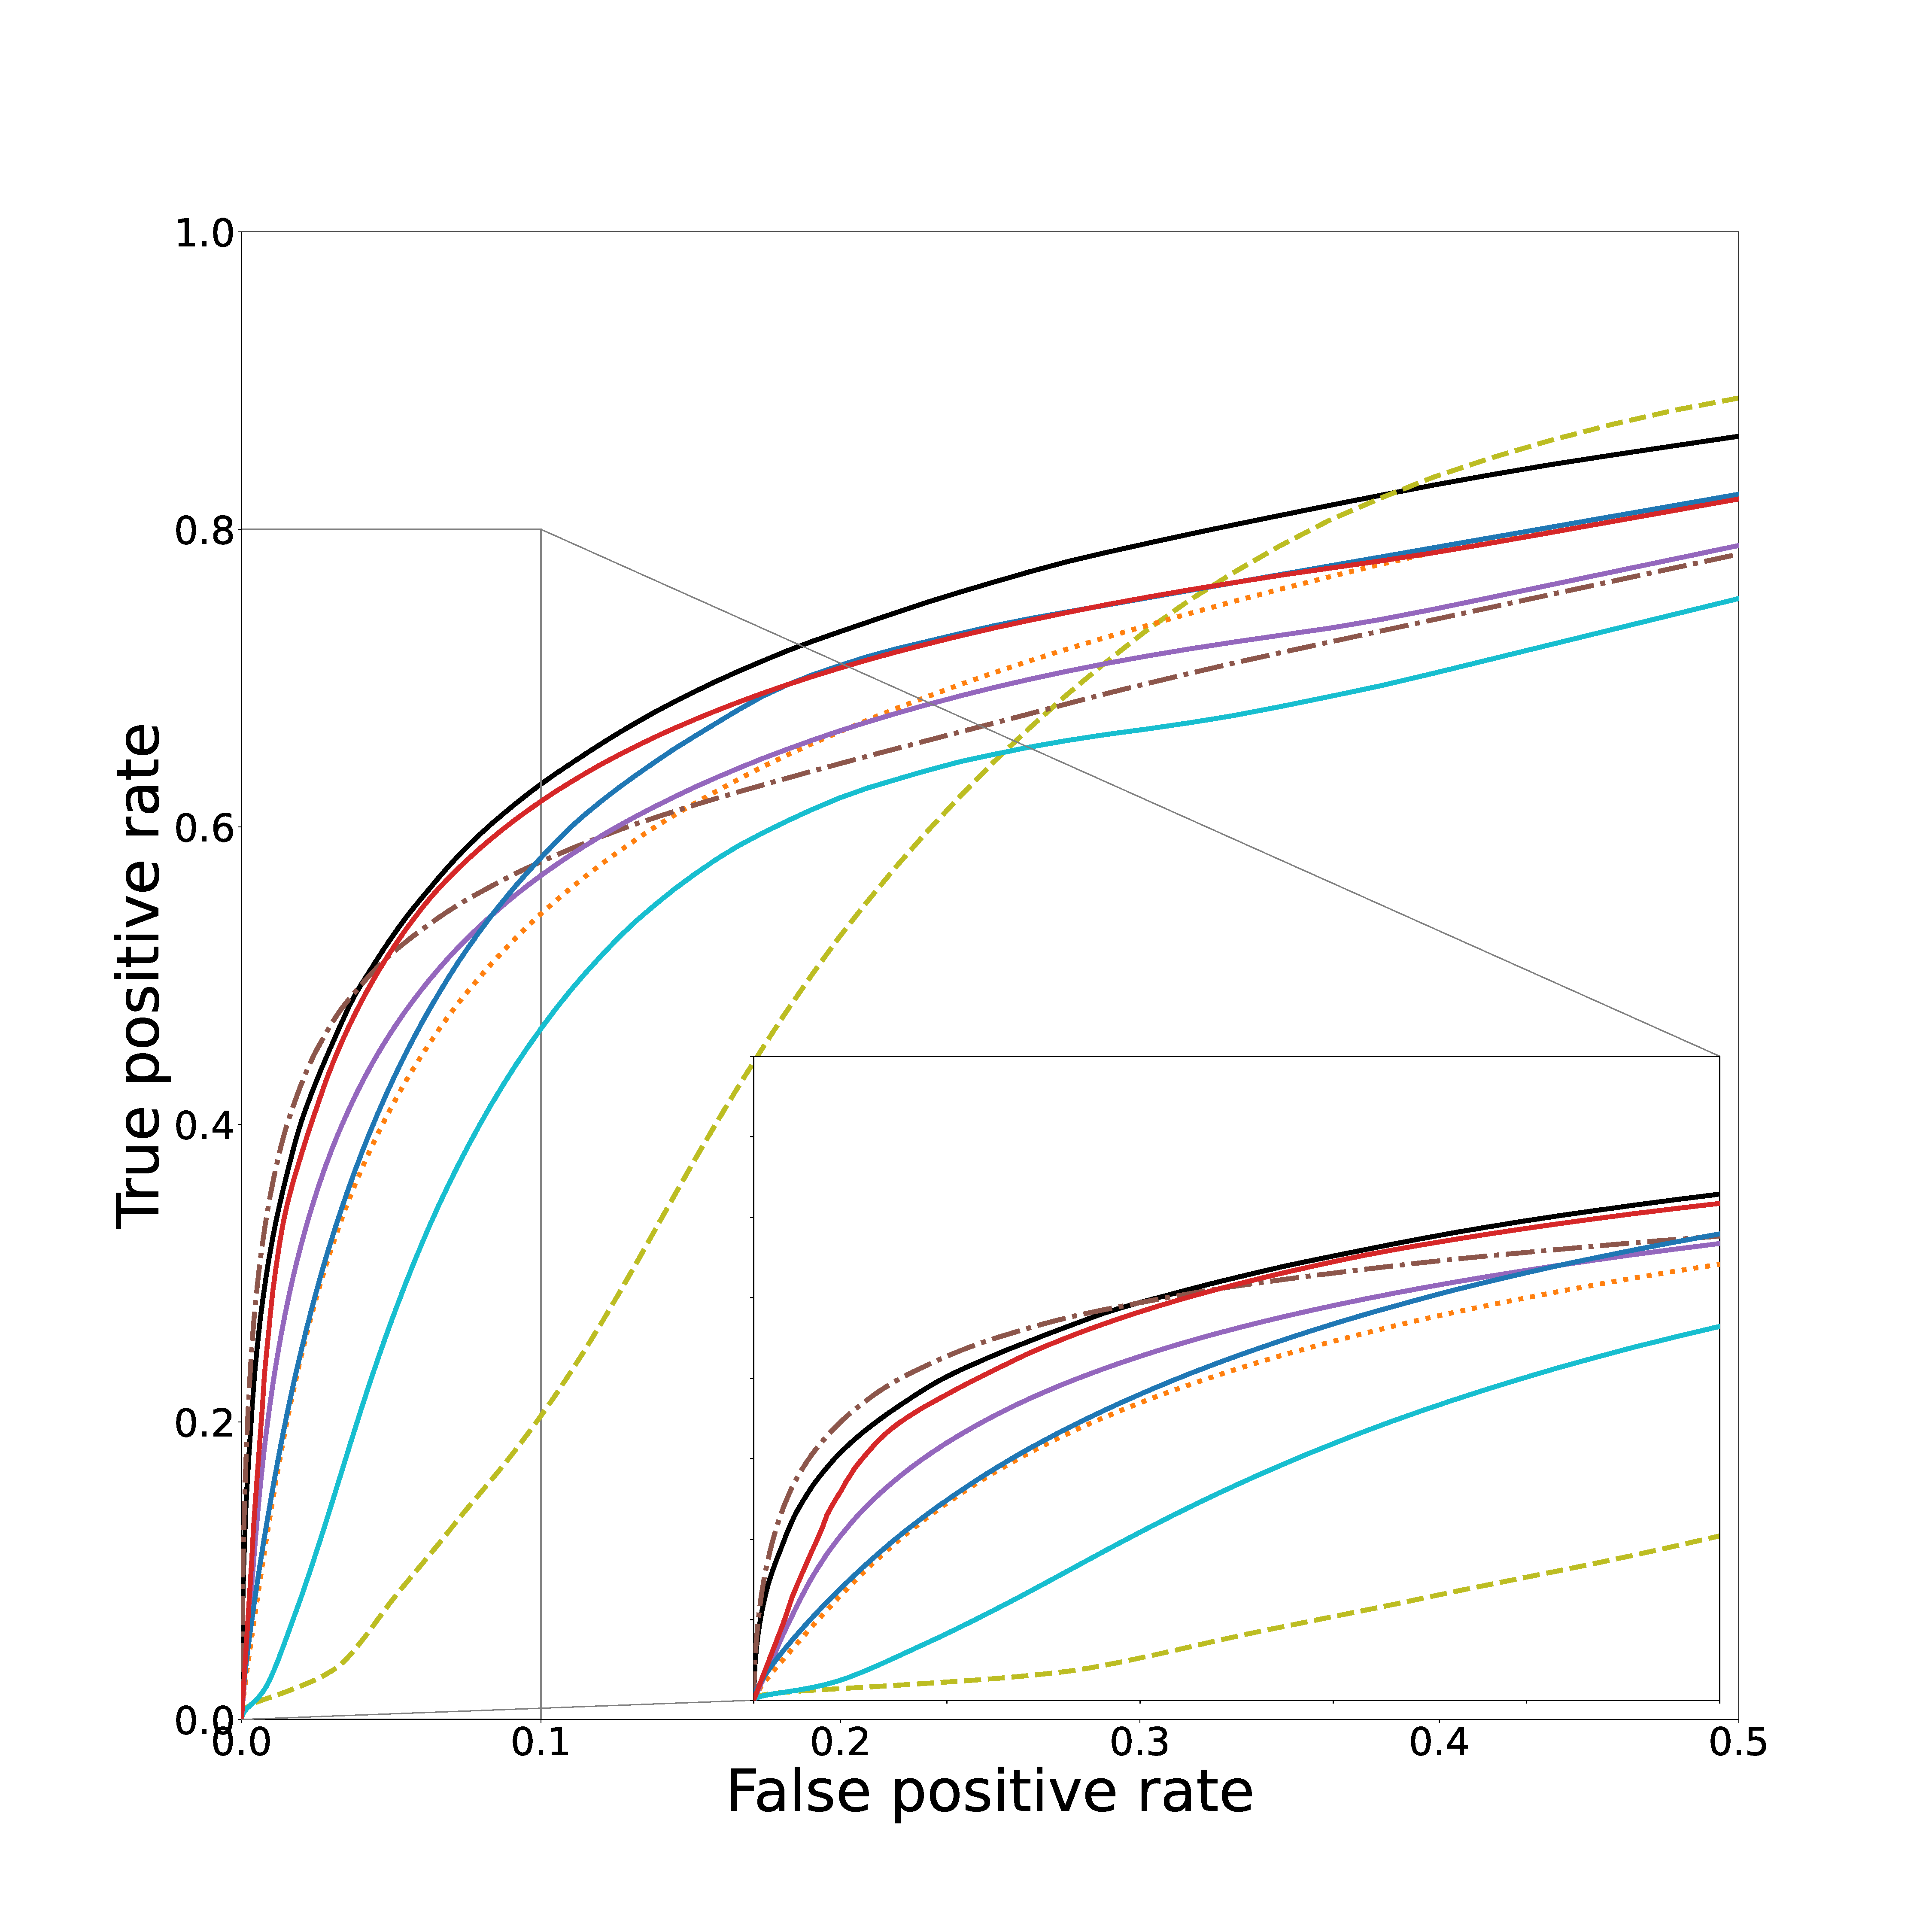
\includegraphics[clip = true, trim  =  125 125 180 260, width=44mm]{Images/Ircad_ROC.pdf}
  \caption{Ircad}
\end{subfigure}
  \begin{subfigure}[t]{0.4\textwidth}
  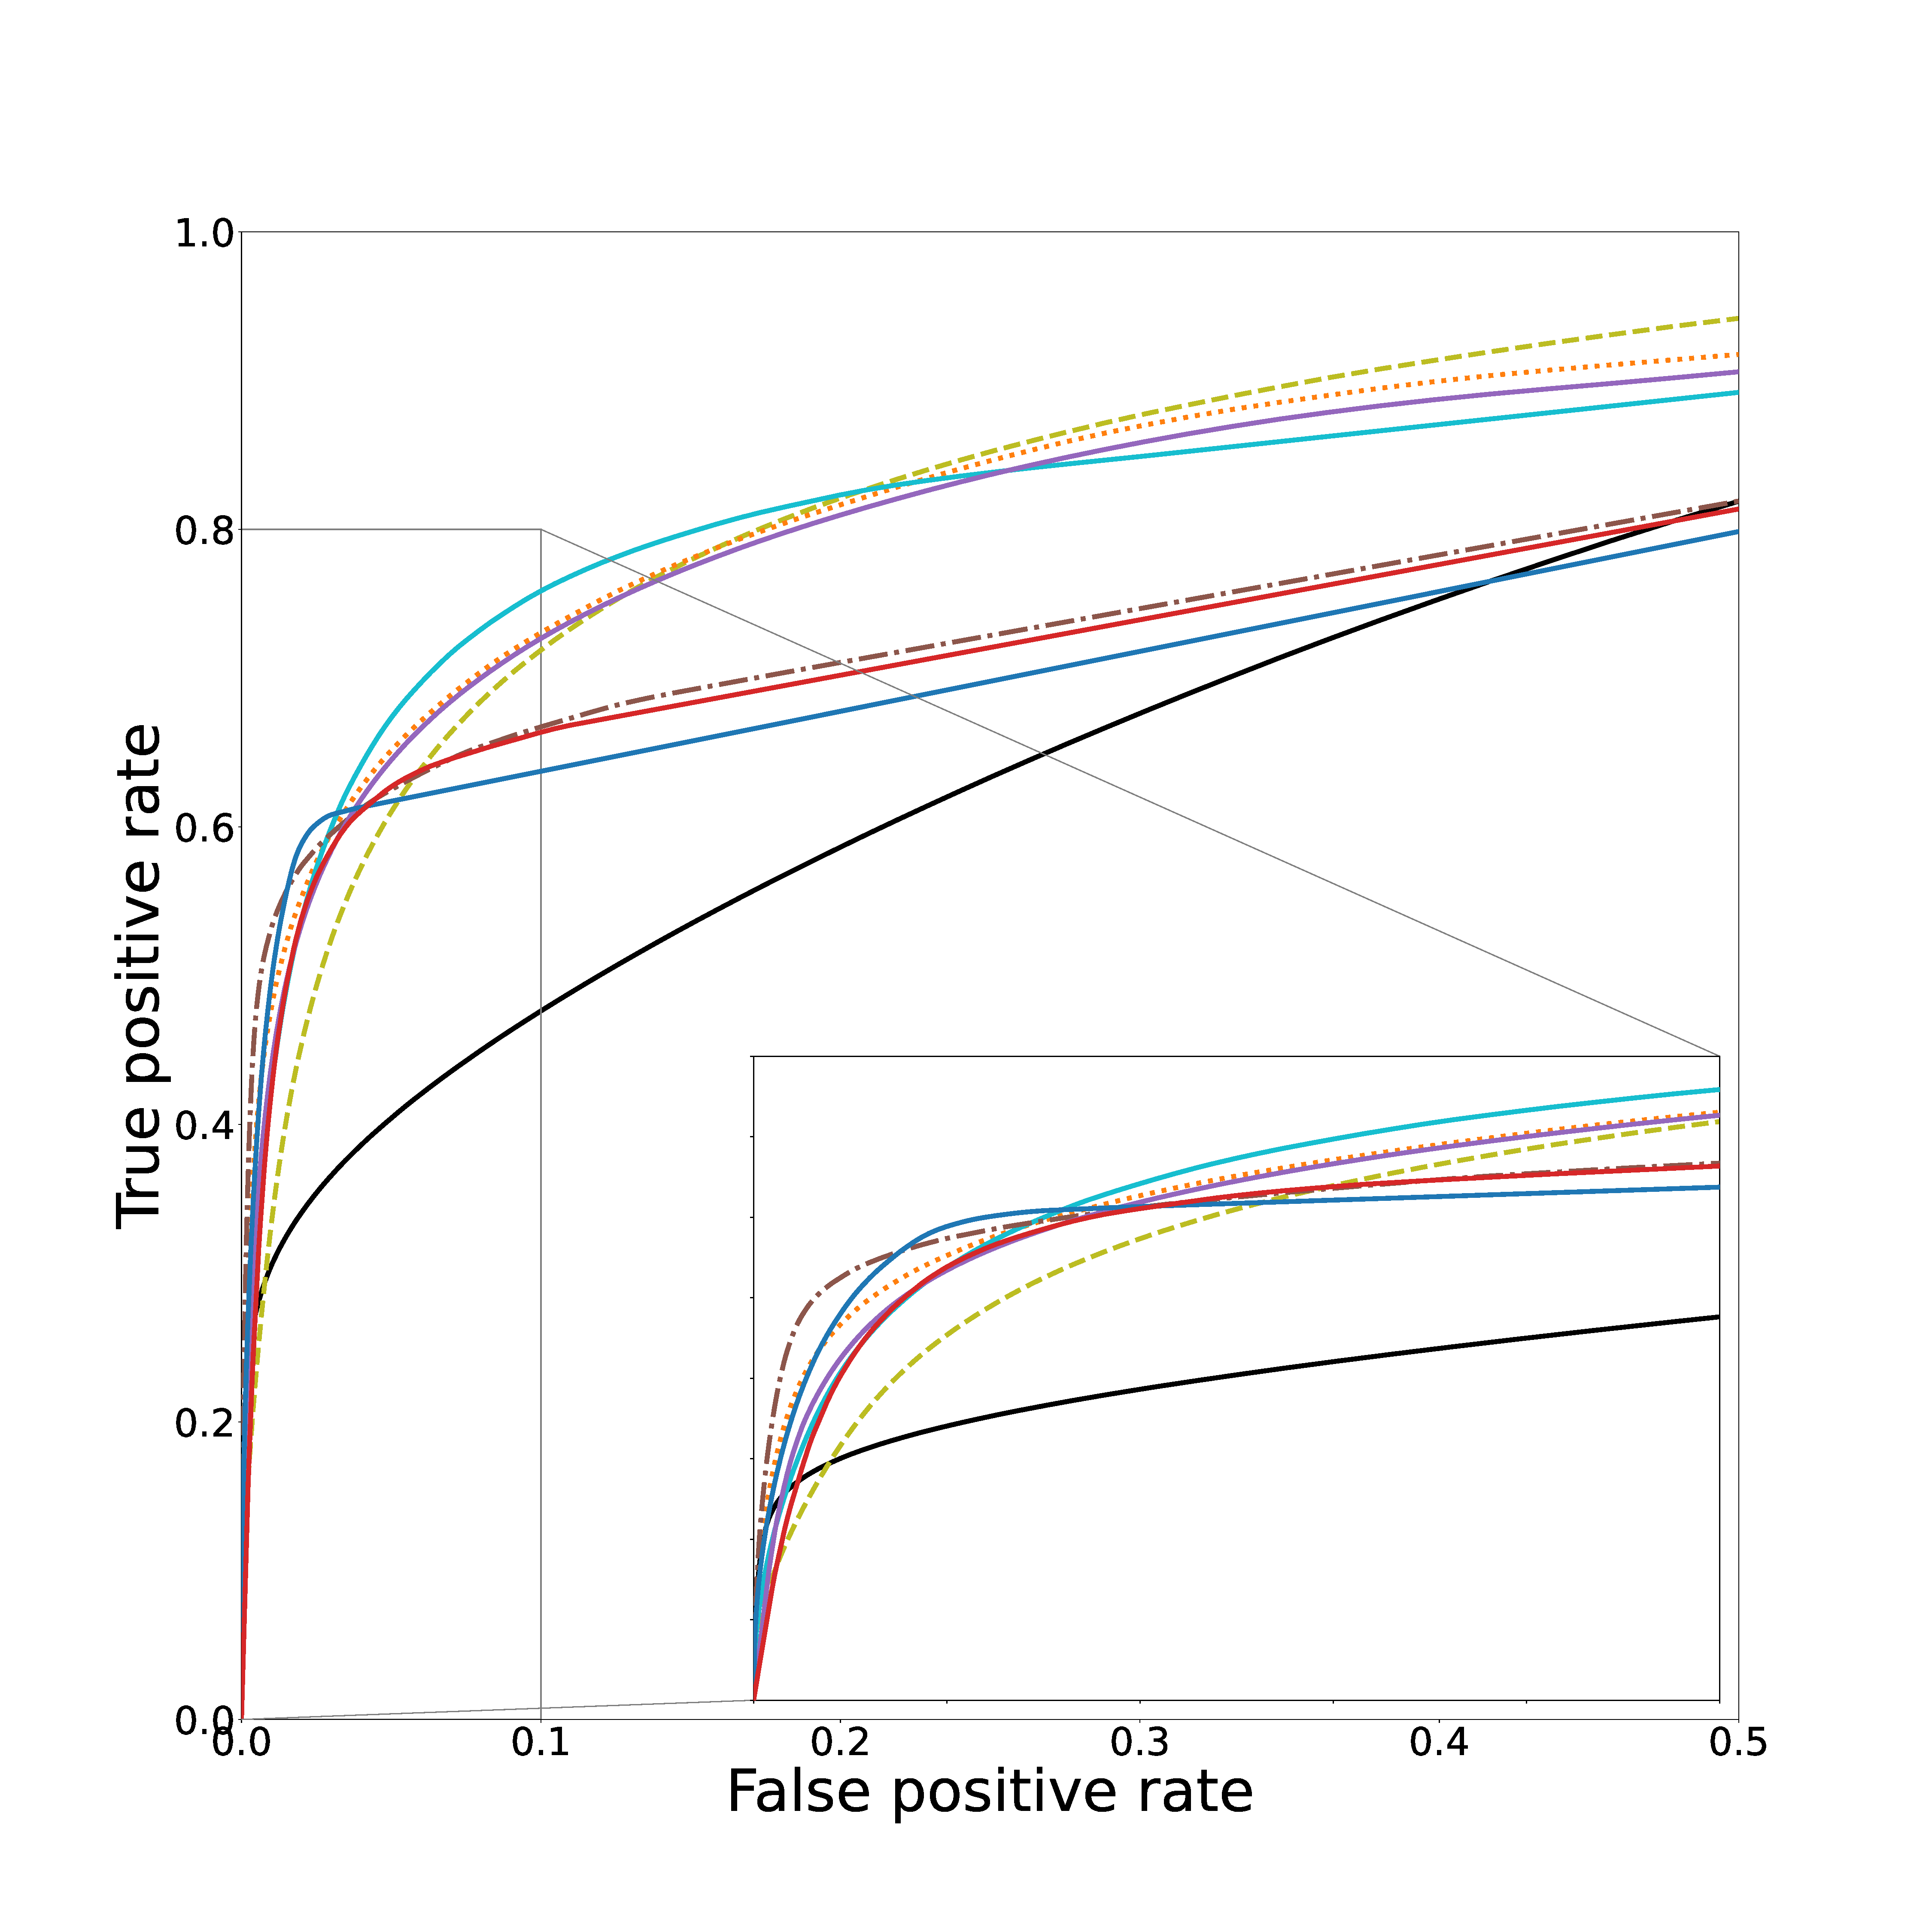
\includegraphics[clip = true, trim  =  125 125 180 200, width=44mm]{Images/Bullitt_ROC.pdf} \\
  \caption{Bullitt}
\end{subfigure}
  \begin{subfigure}[t]{0.4\textwidth}
  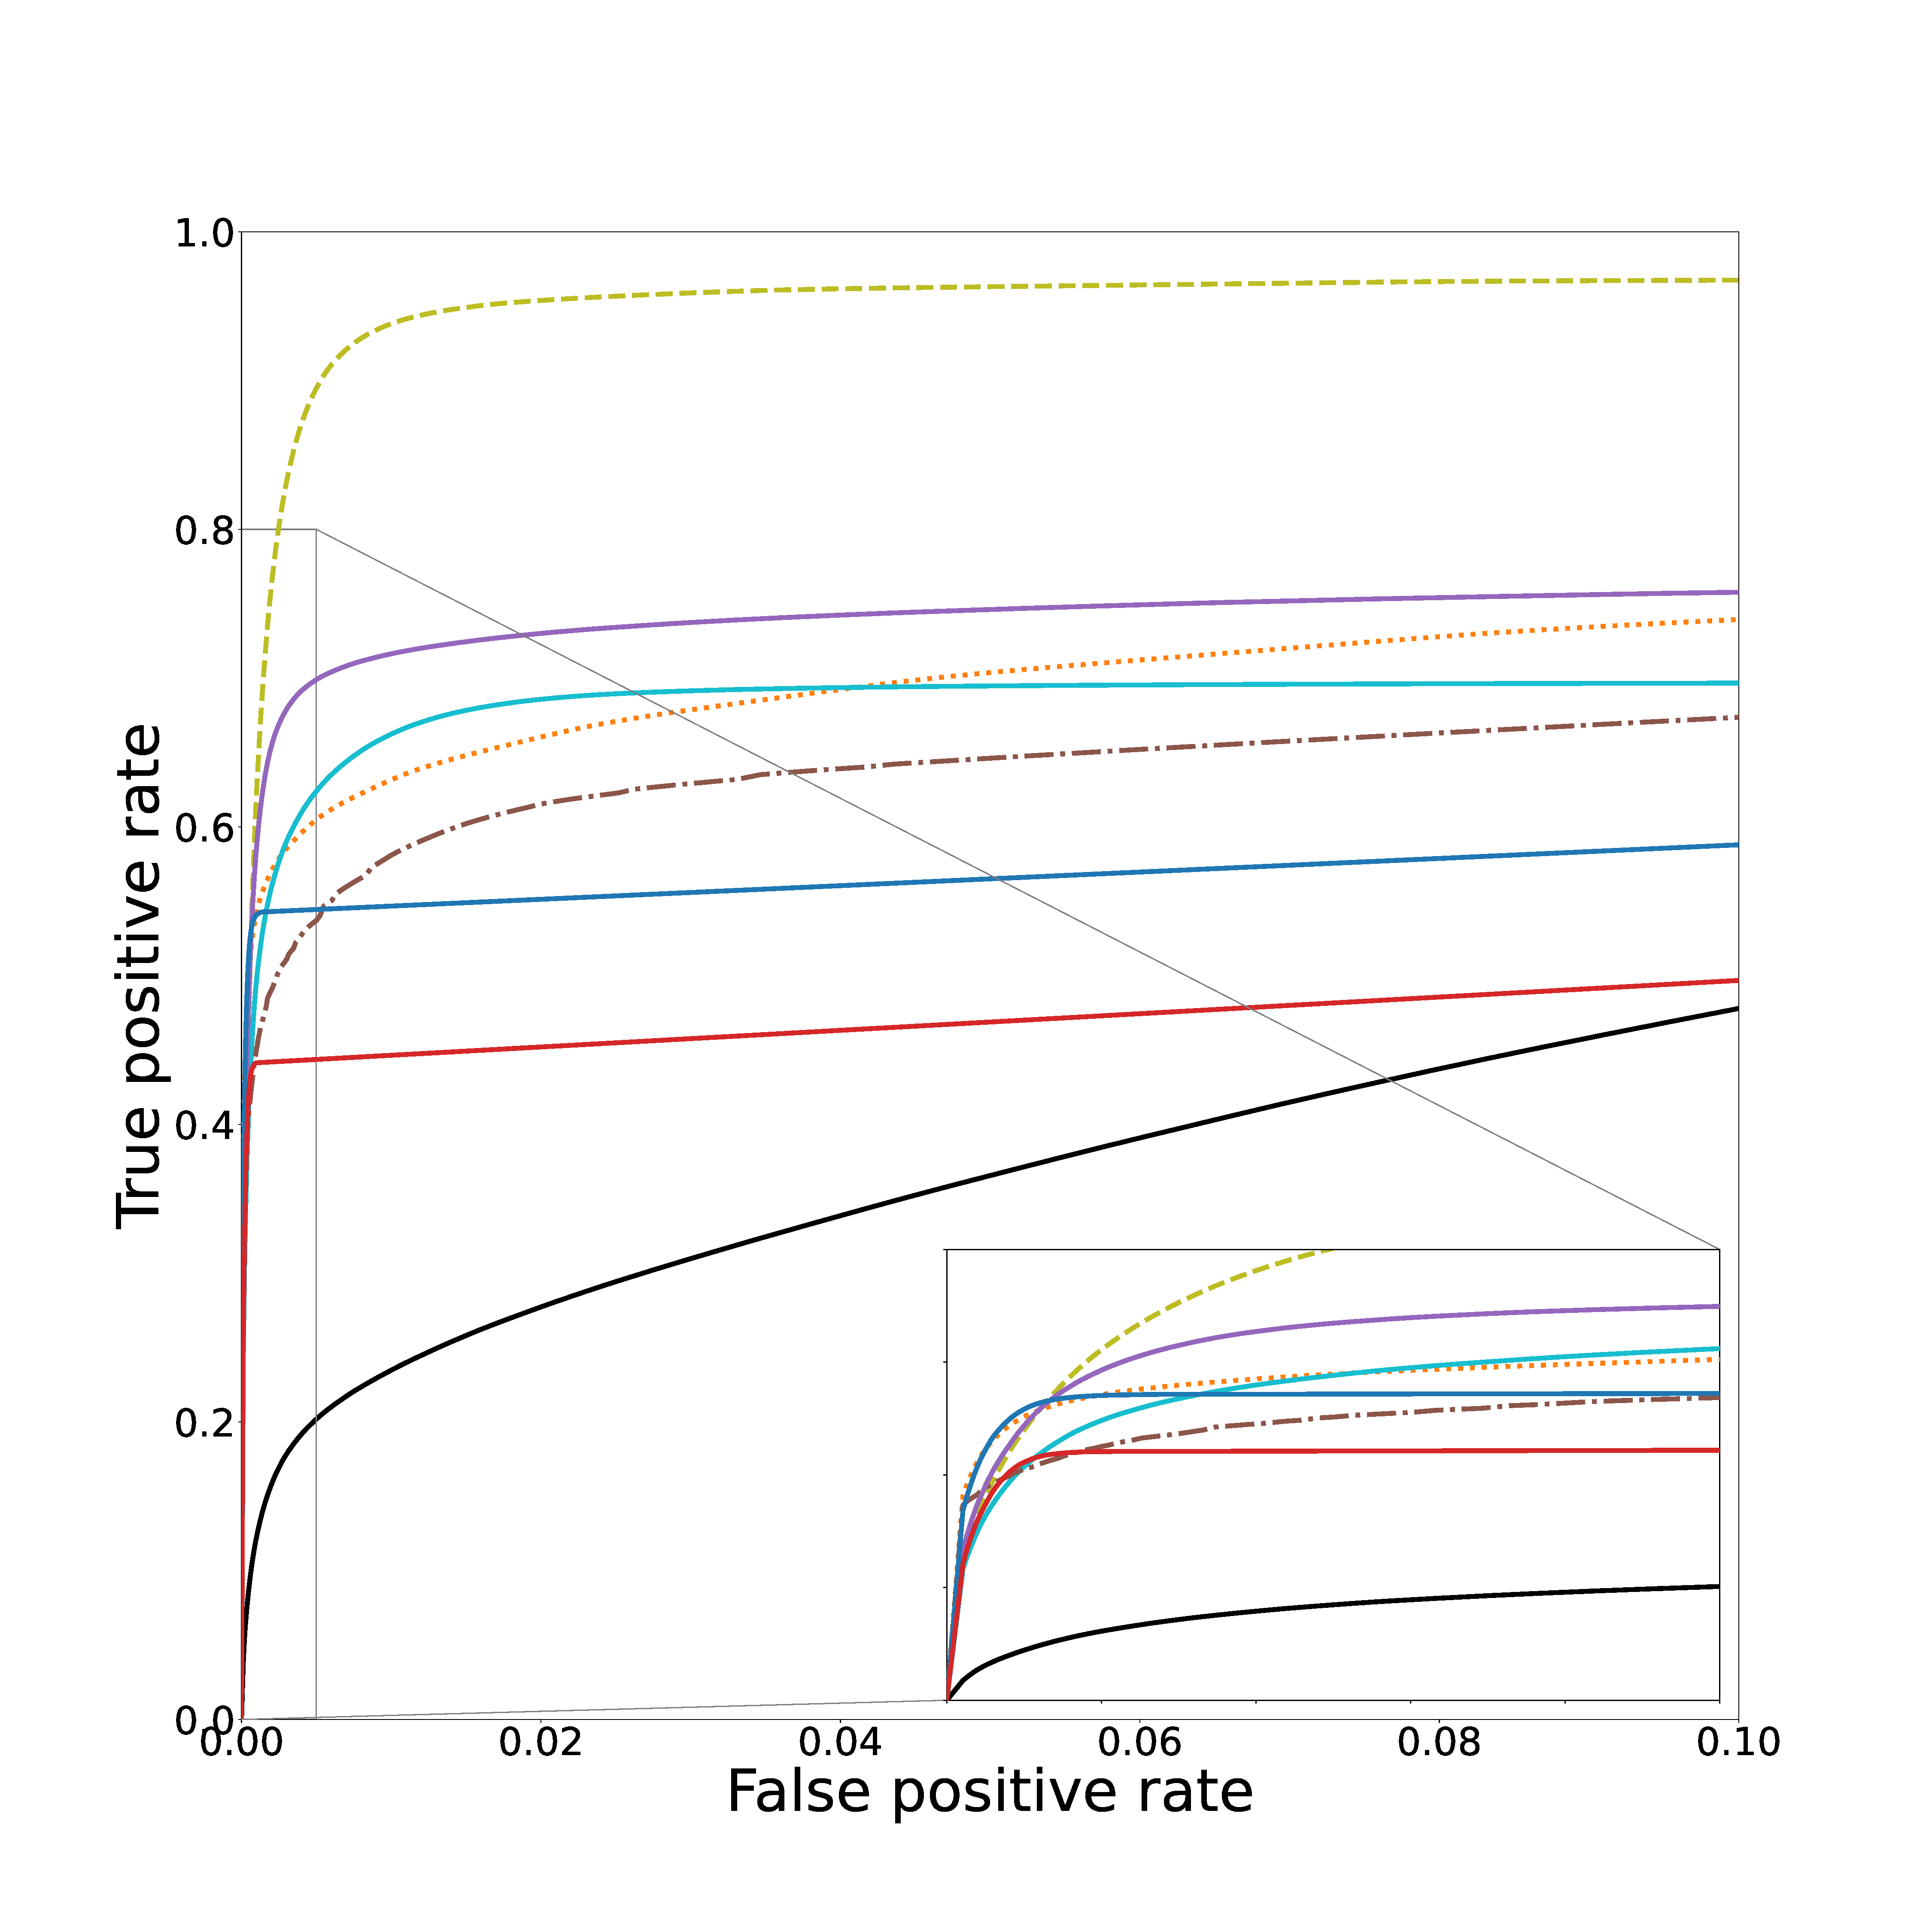
\includegraphics[clip = true, trim  =  125 125 100 200, width=44mm]{Images/Vascu_2_ROC.pdf}
  \caption{VascuSynth, $\sigma = 2$}
\end{subfigure}
  \begin{subfigure}[t]{0.4\textwidth}
  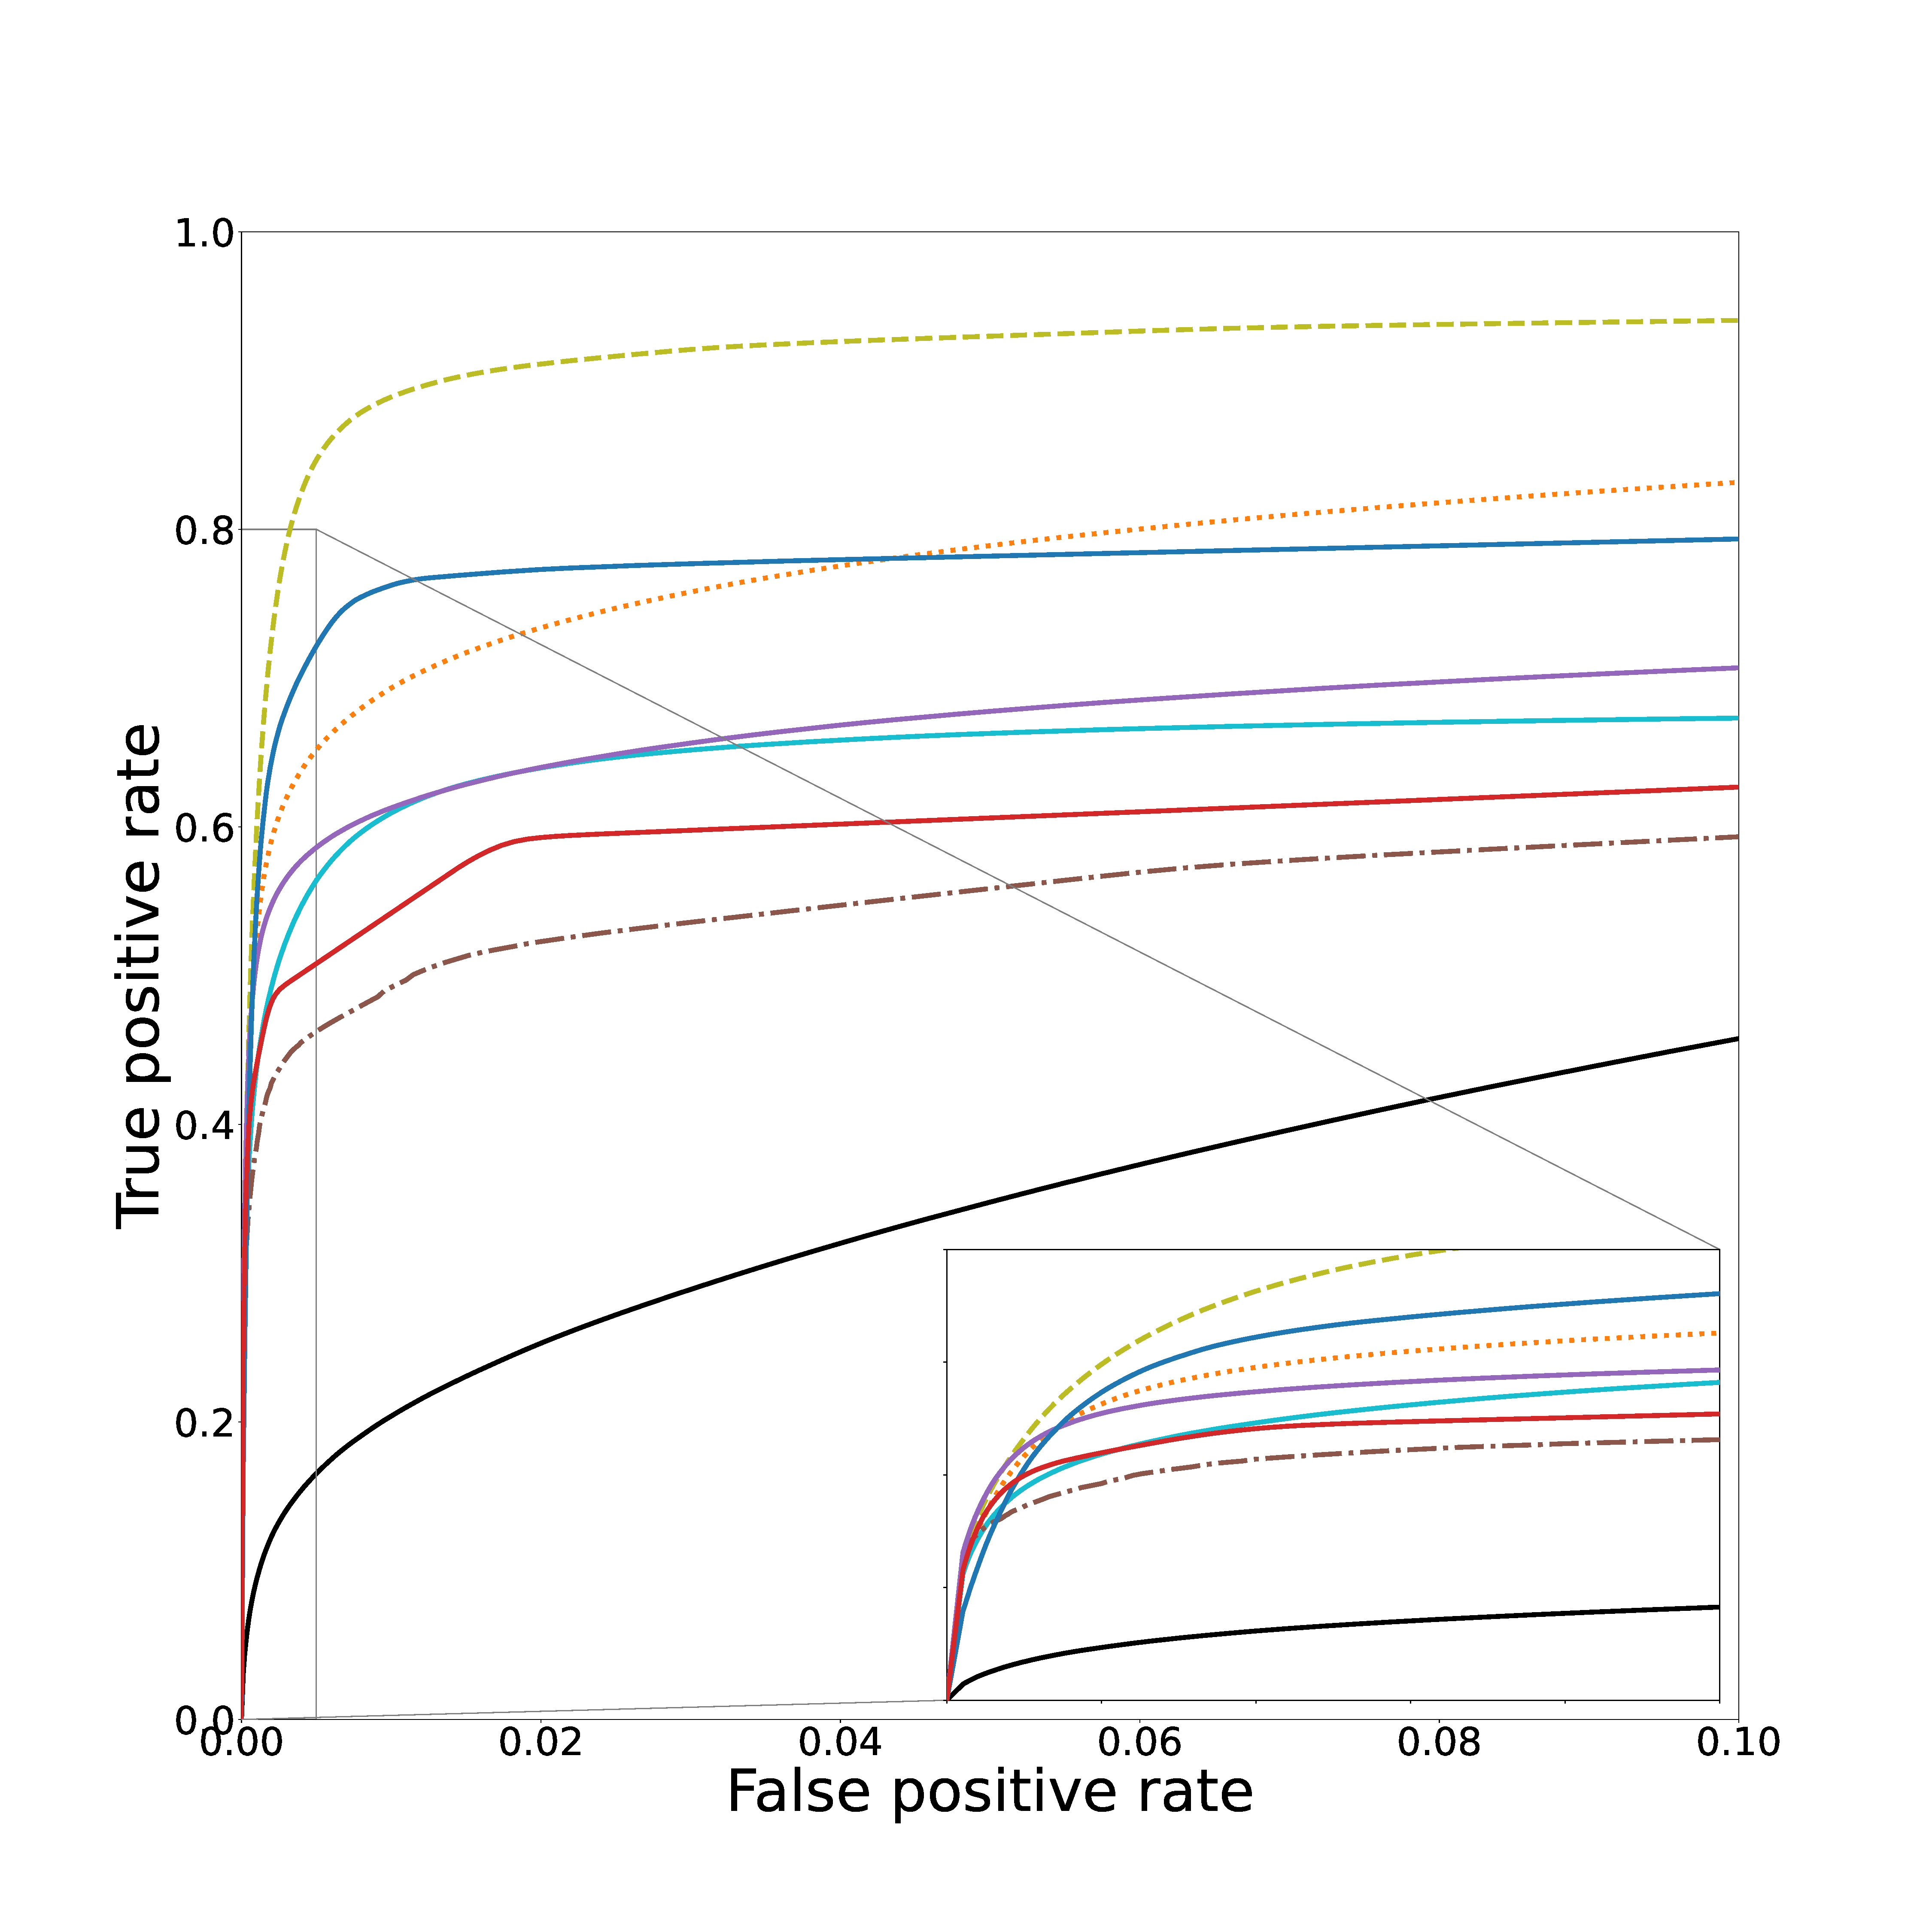
\includegraphics[clip = true, trim  =  125 125 100 200, width=44mm]{Images/Vascu_4_ROC.pdf}
  \caption{VascuSynth, $\sigma = 4$}
\end{subfigure}
  \begin{subfigure}[t]{0.4\textwidth}
    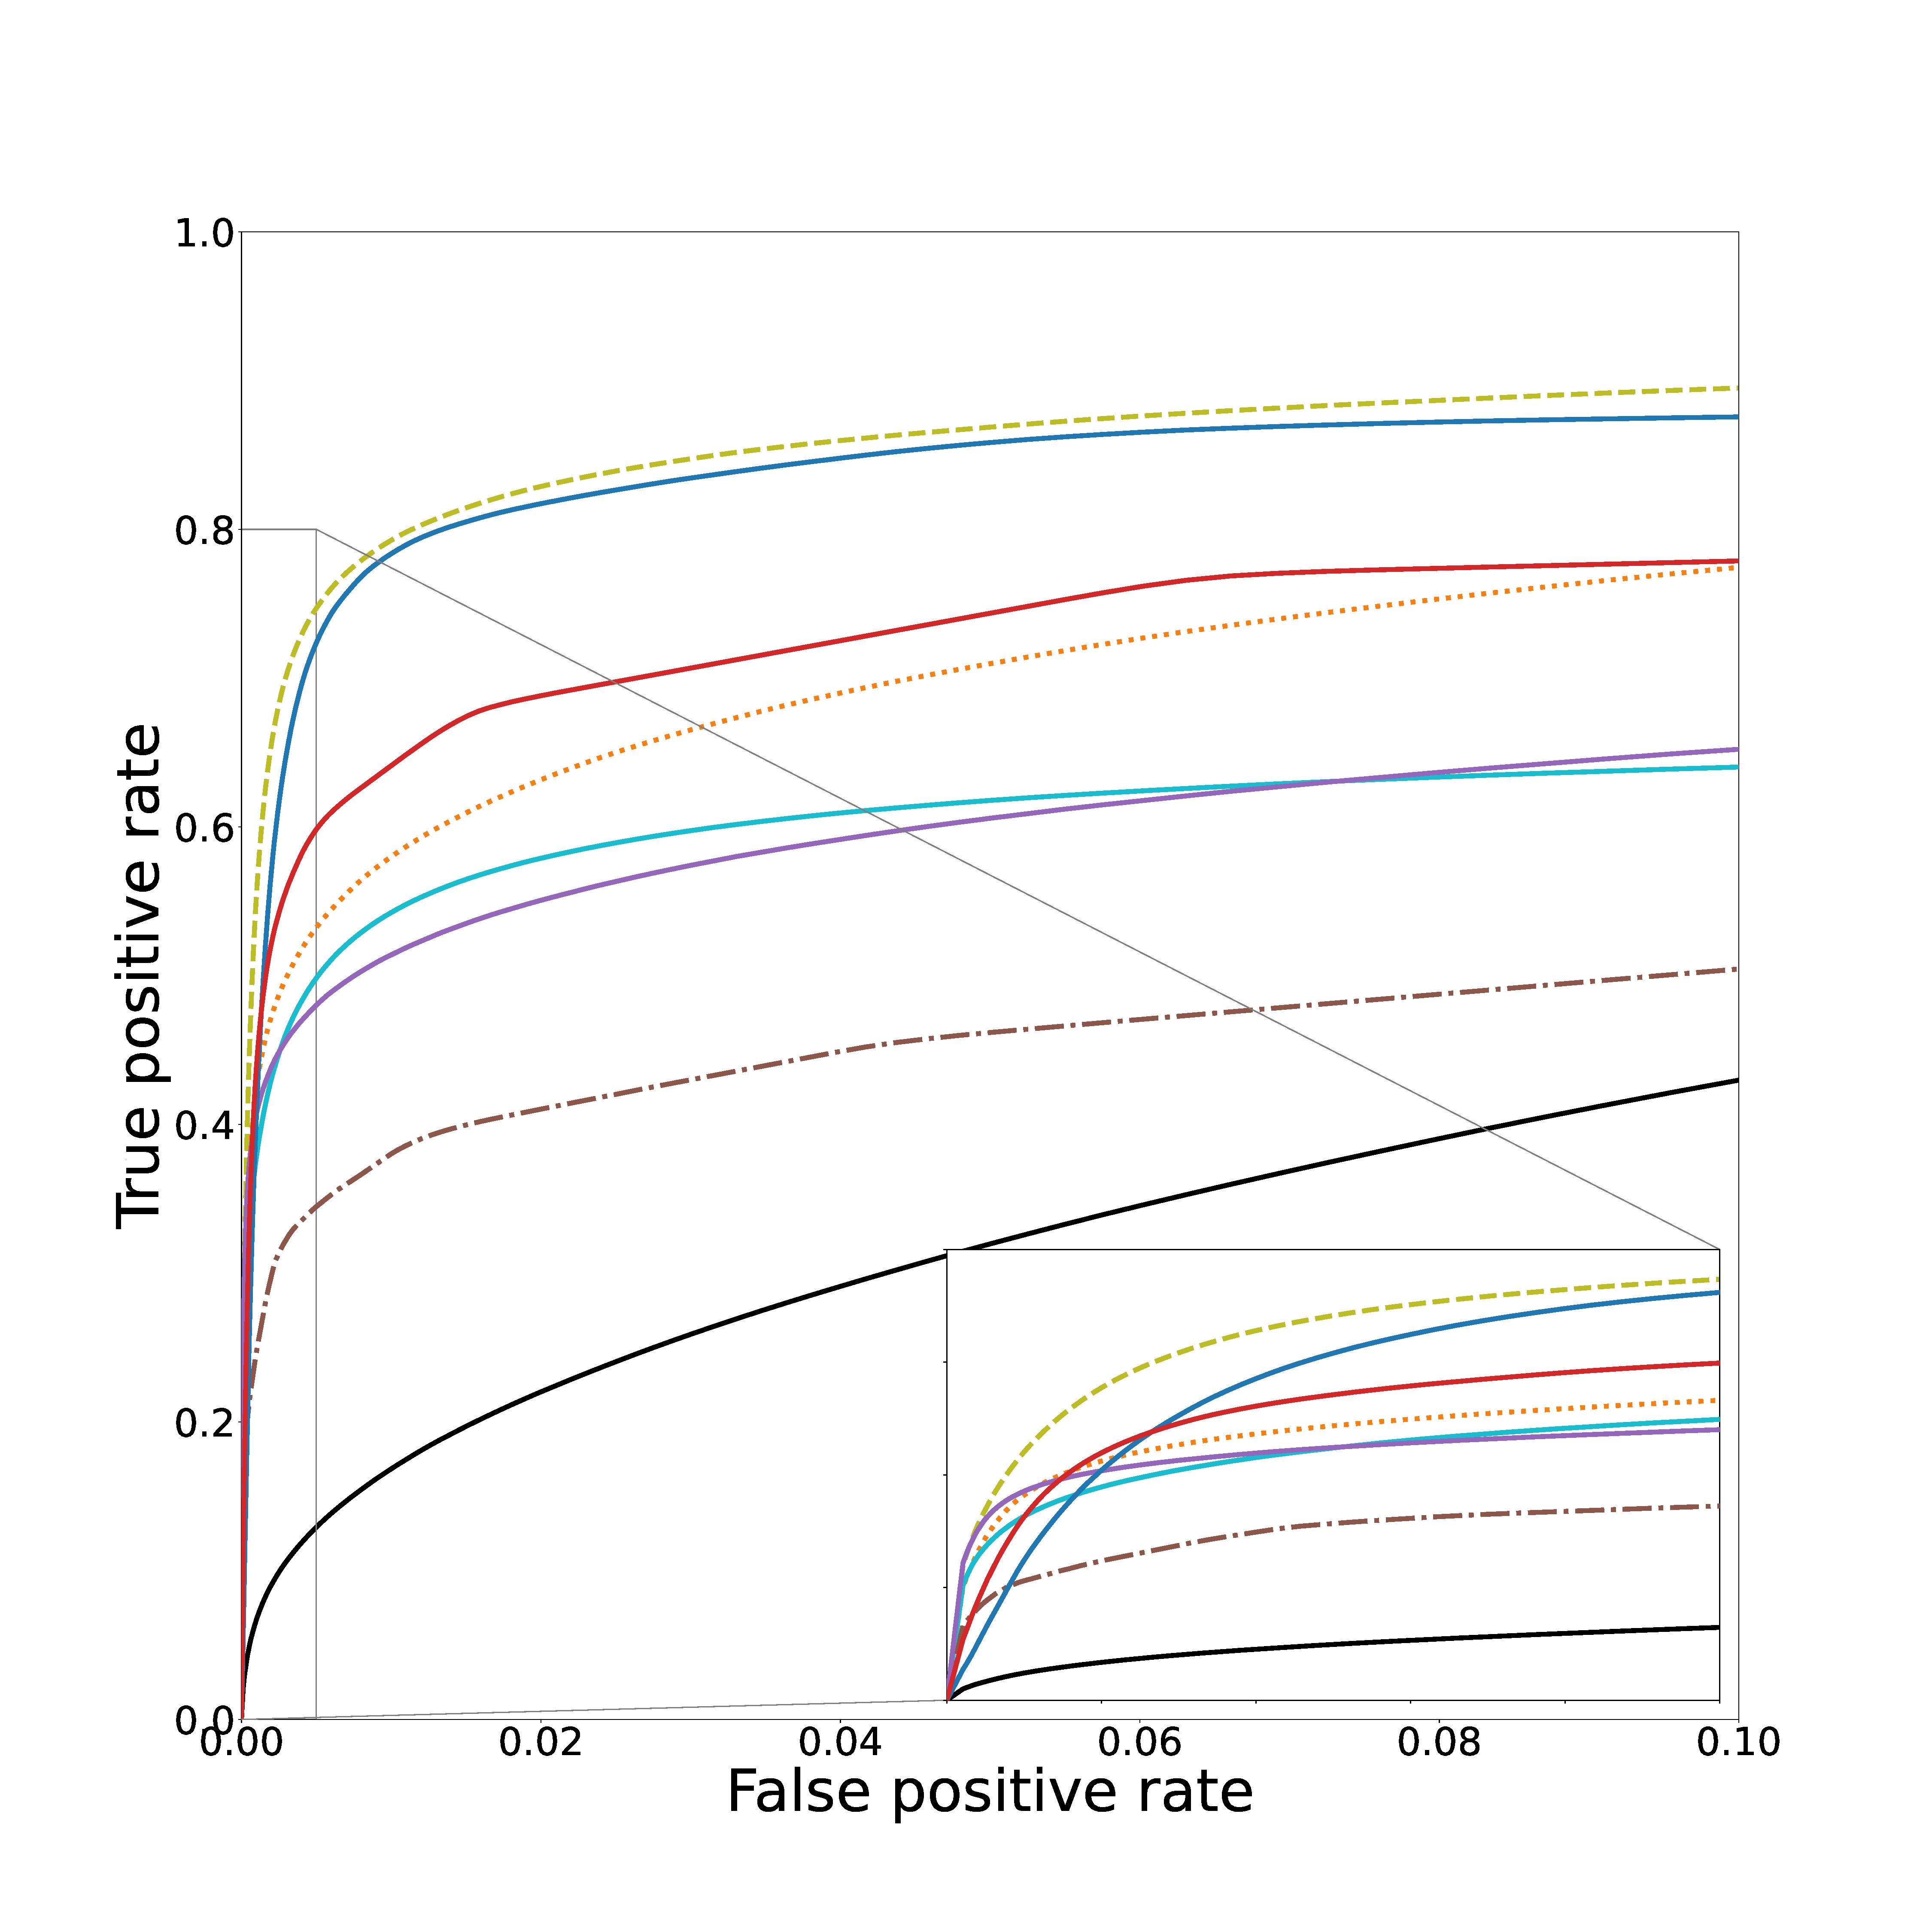
\includegraphics[clip = true, trim  =  125 125 100 200, width=44mm]{Images/Vascu_6_ROC.pdf}
    \caption{VascuSynth, $\sigma = 6$}
\end{subfigure}
  \caption{
    courbe ROC moyenne des sept de rehaussement pour (b) le jeu de l'Ircad,  (c) Bullitt (d--f) et les jeux de données de VascuSynth pour les 3 niveaux de bruit.
    Les courbes ROC sont zoomés puisque les vaisseaux représentent respectivement $6.4$ pourcent (b), $1.7$ pourcent (c), et $0.2$ pourcent (d--f) du nombre total de voxels.
    }
  \label{fig:Ircad_vascu_bullitt_ROC}
\end{figure}


\begin{figure}[!ht]
  \centering
  % ground truth
  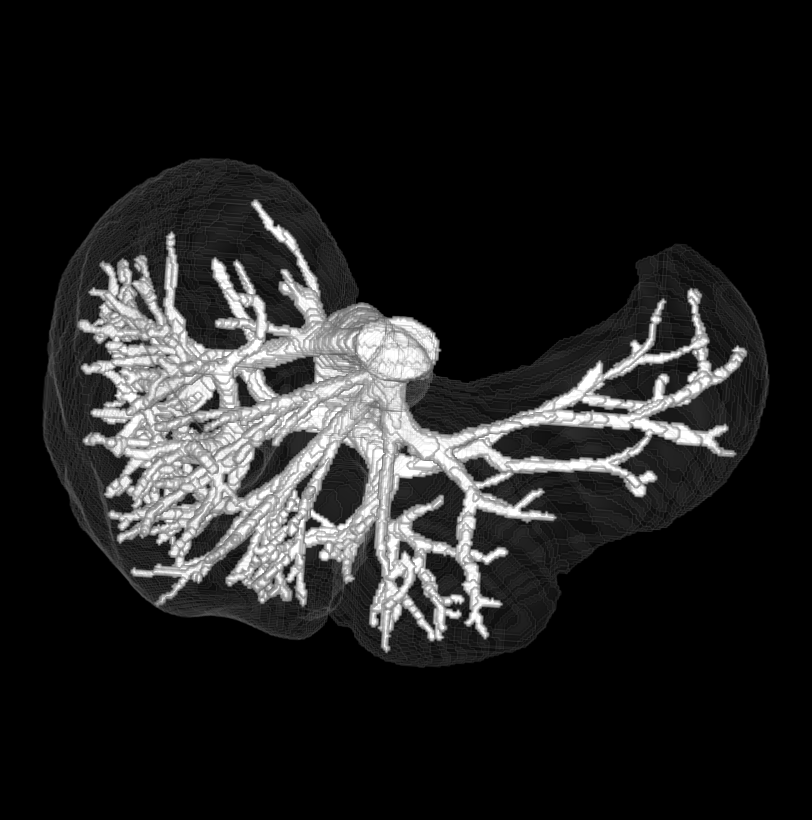
\includegraphics[clip = true, trim  =  10 150 10 150, height=25mm,width=36mm]{Images/Ircad_GT.png}
  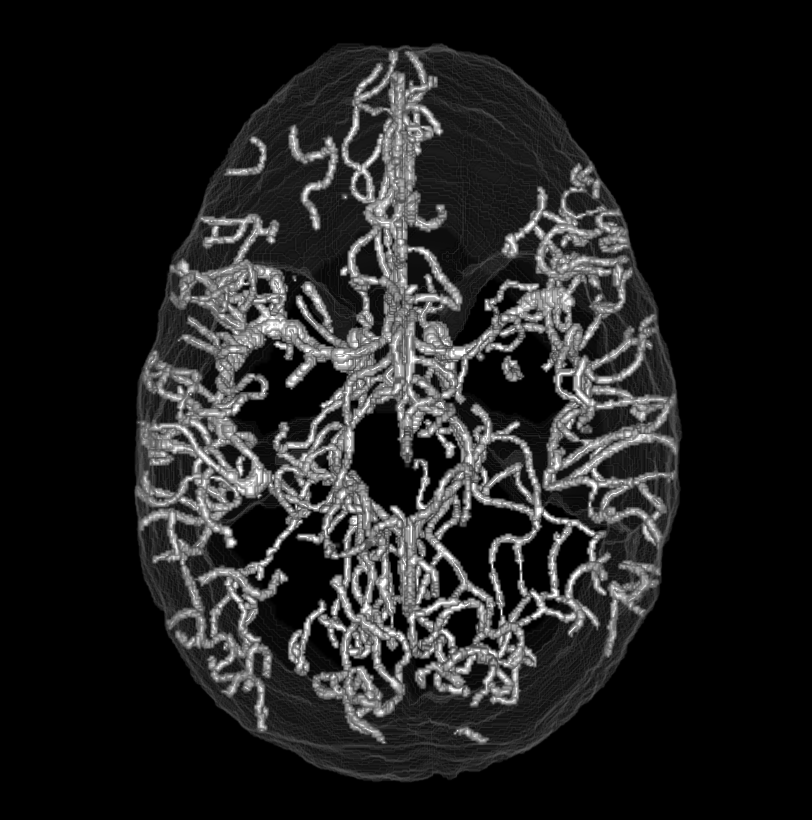
\includegraphics[clip = true, trim = 90 20 90 20, height=25mm,width=24mm]{Images/Bullitt_GT.png}
  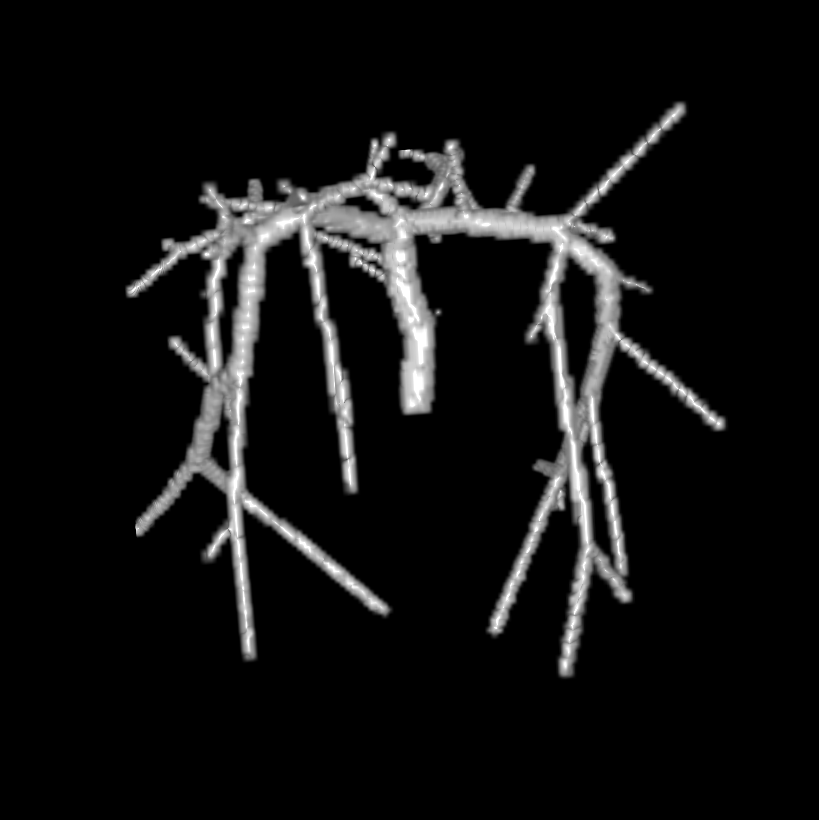
\includegraphics[clip = true, trim = 80 80 80 80, height=25mm]{Images/Vascu_4_GT.png}
  \\
  % Baseline
  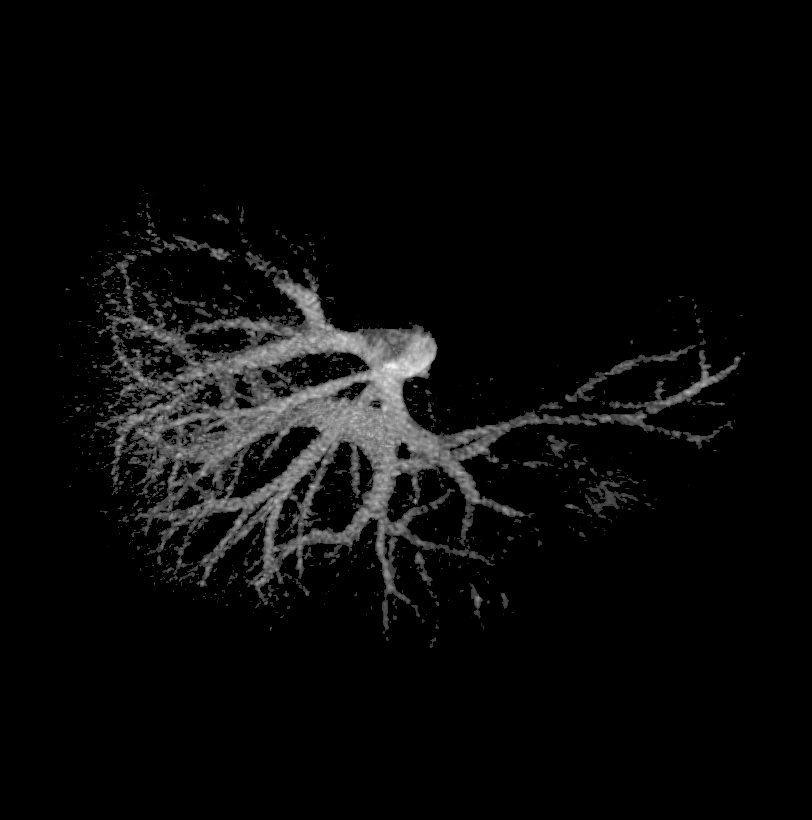
\includegraphics[clip = true, trim  =  10 150 10 150, height=25mm,width=36mm]{Images/Ircad_Baseline.png}
  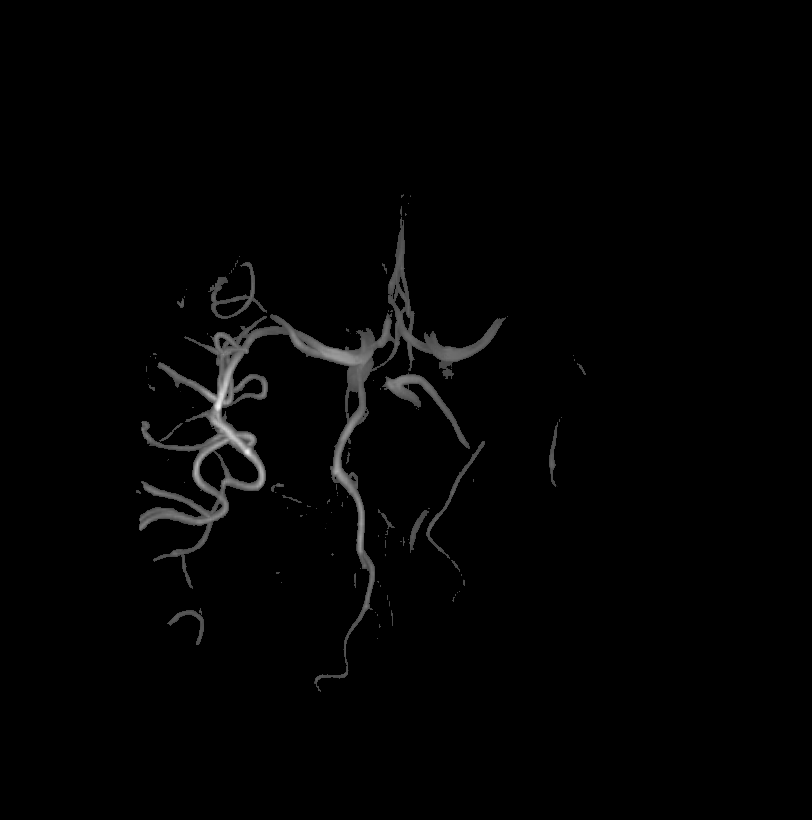
\includegraphics[clip = true, trim = 90 20 90 20, height=25mm,width=24mm]{Images/Bullitt_Baseline.png}
  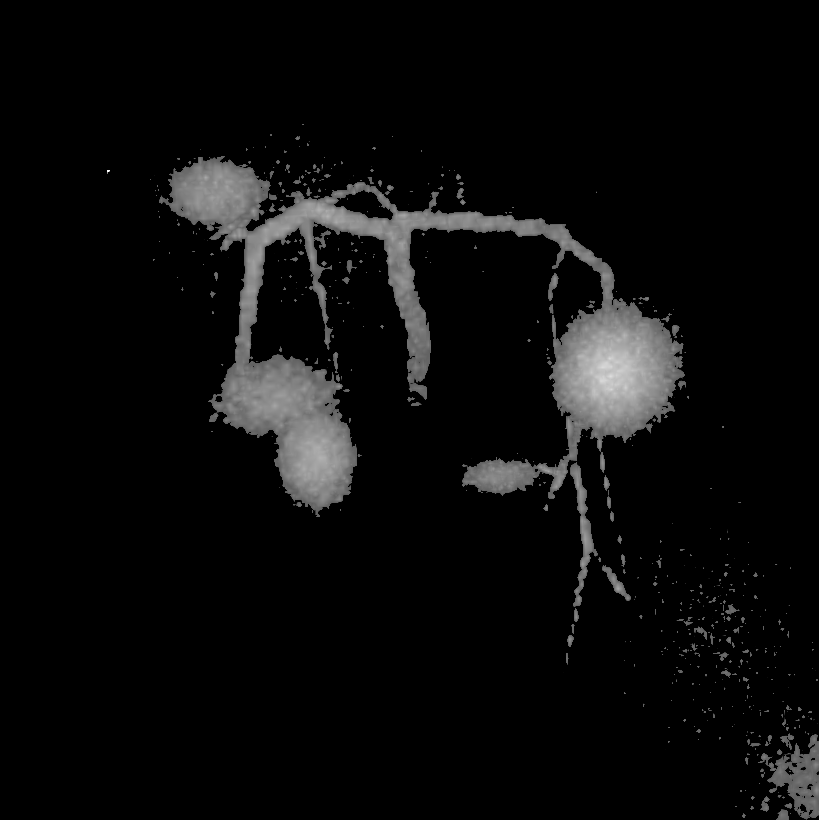
\includegraphics[clip = true, trim = 80 80 80 80,, height=25mm]{Images/Vascu_4_Baseline.png}
  \\
  % Frangi
  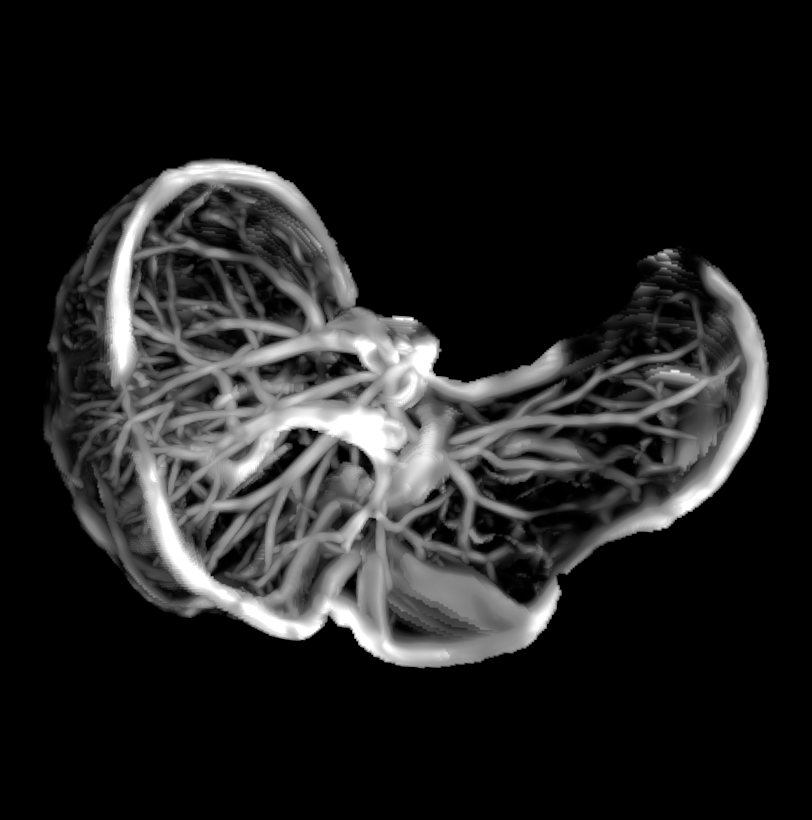
\includegraphics[clip = true, trim  =  10 150 10 150, height=25mm,width=36mm]{Images/Ircad_Frangi.png}
  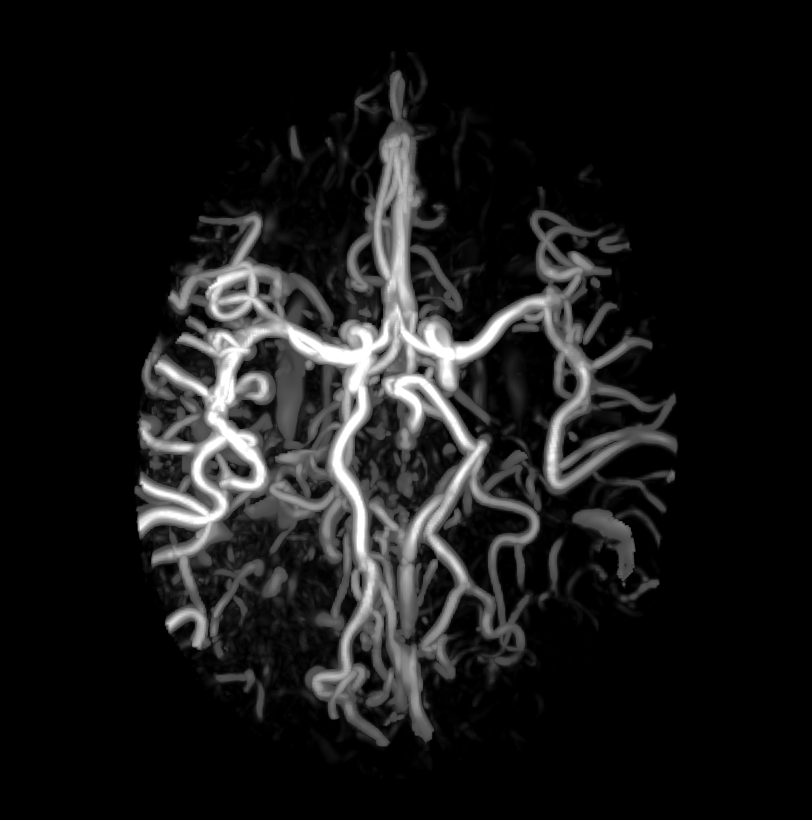
\includegraphics[clip = true, trim = 90 20 90 20, height=25mm,width=24mm]{Images/Bullitt_Frangi.png}
  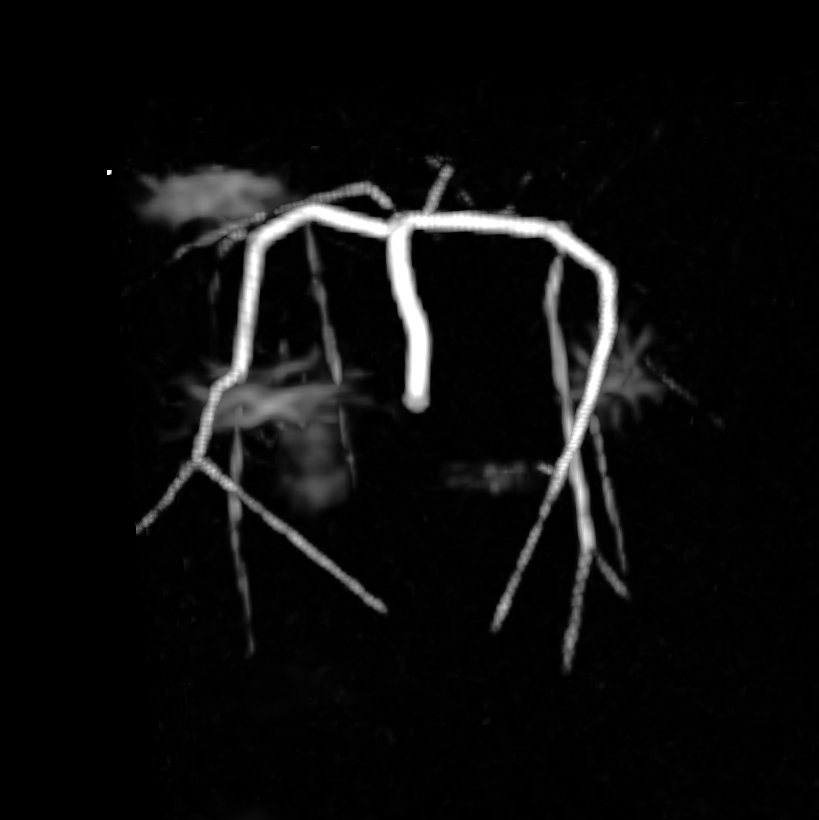
\includegraphics[clip = true, trim = 80 80 80 80,, height=25mm]{Images/Vascu_4_Frangi.png}
  \\
  % Jerman
  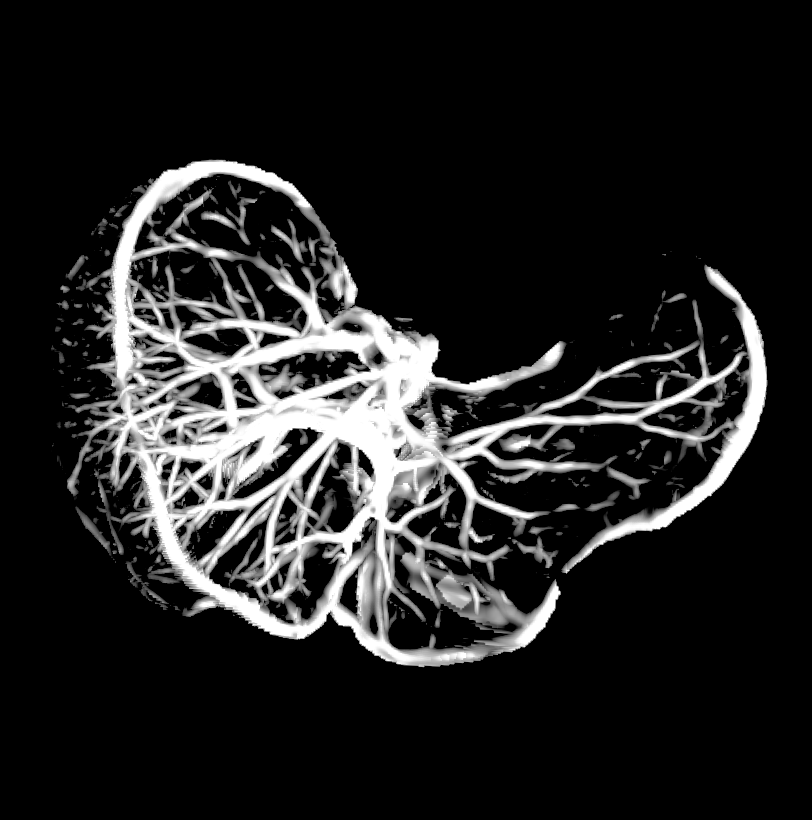
\includegraphics[clip = true, trim  =  10 150 10 150, height=25mm,width=36mm]{Images/Ircad_Jerman.png}
  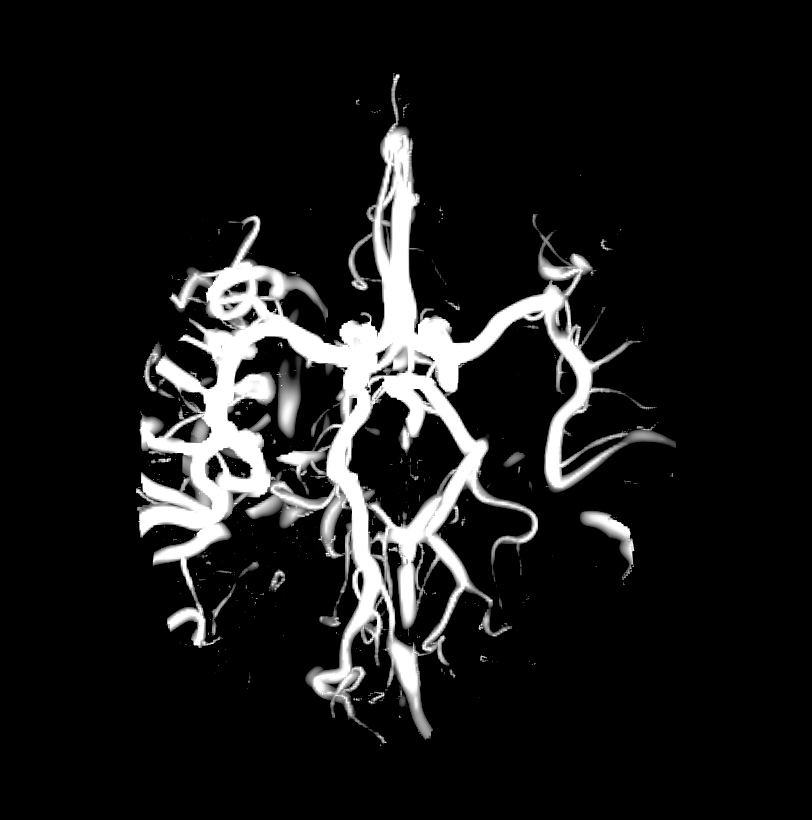
\includegraphics[clip = true, trim = 90 20 90 20, height=25mm,width=24mm]{Images/Bullitt_Jerman.png}
  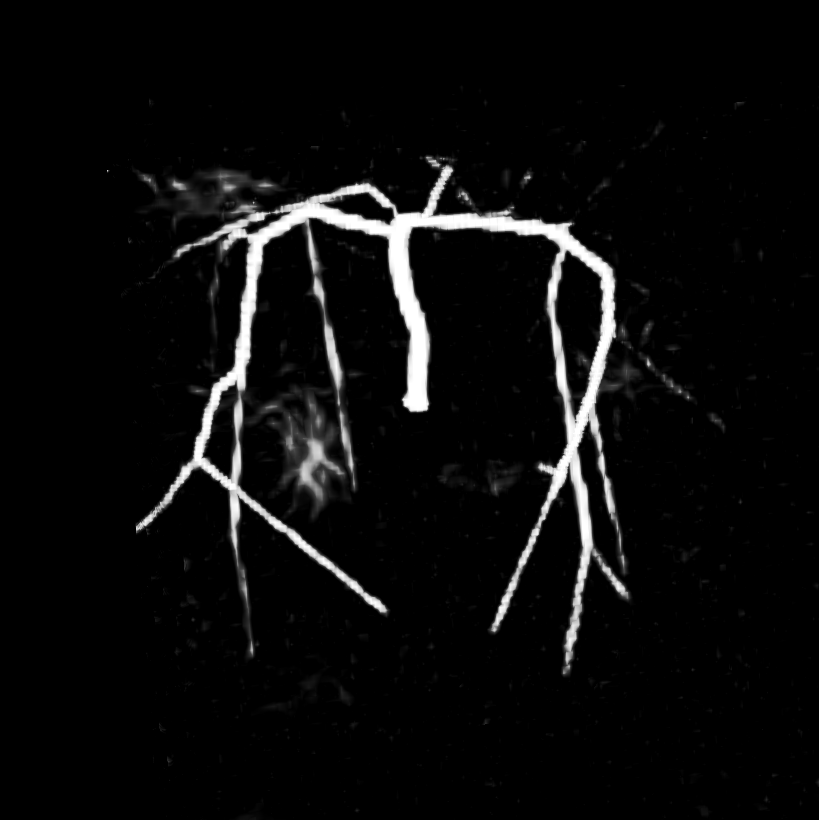
\includegraphics[clip = true, trim = 80 80 80 80,, height=25mm]{Images/Vascu_4_Jerman.png}
  \\
  % OOF
  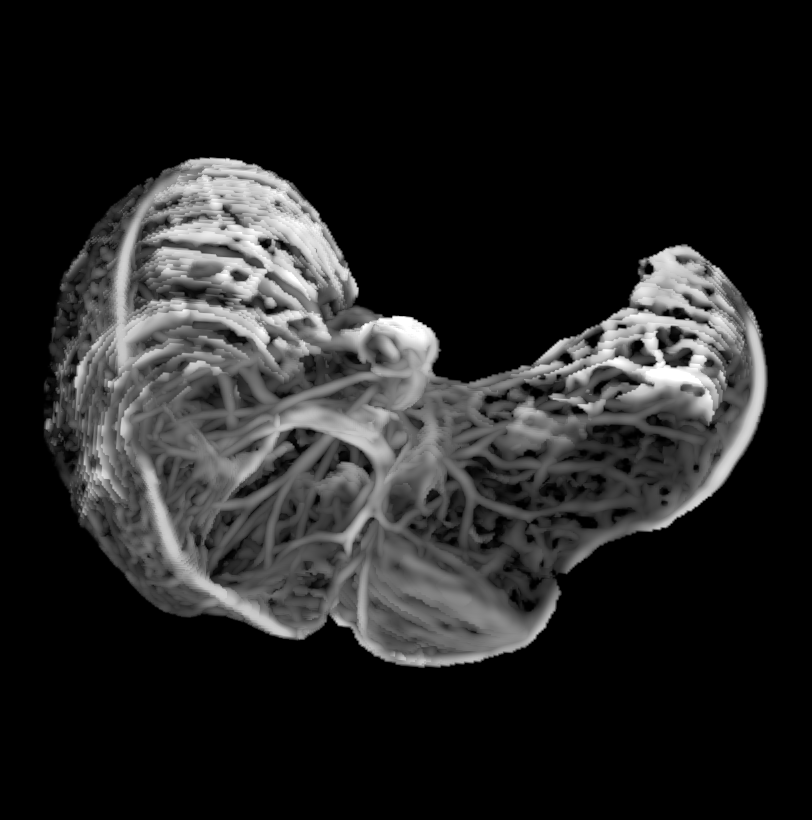
\includegraphics[clip = true, trim  =  10 150 10 150, height=25mm,width=36mm]{Images/Ircad_OOF_GM.png}
  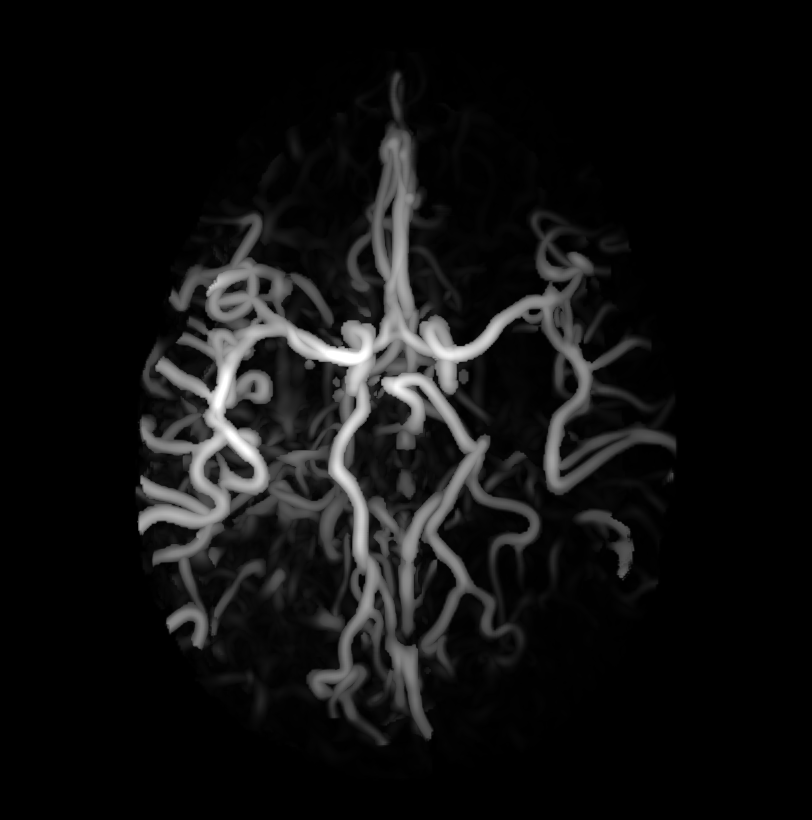
\includegraphics[clip = true, trim = 90 20 90 20,  height=25mm,width=24mm]{Images/Bullitt_OOF_GM.png}
  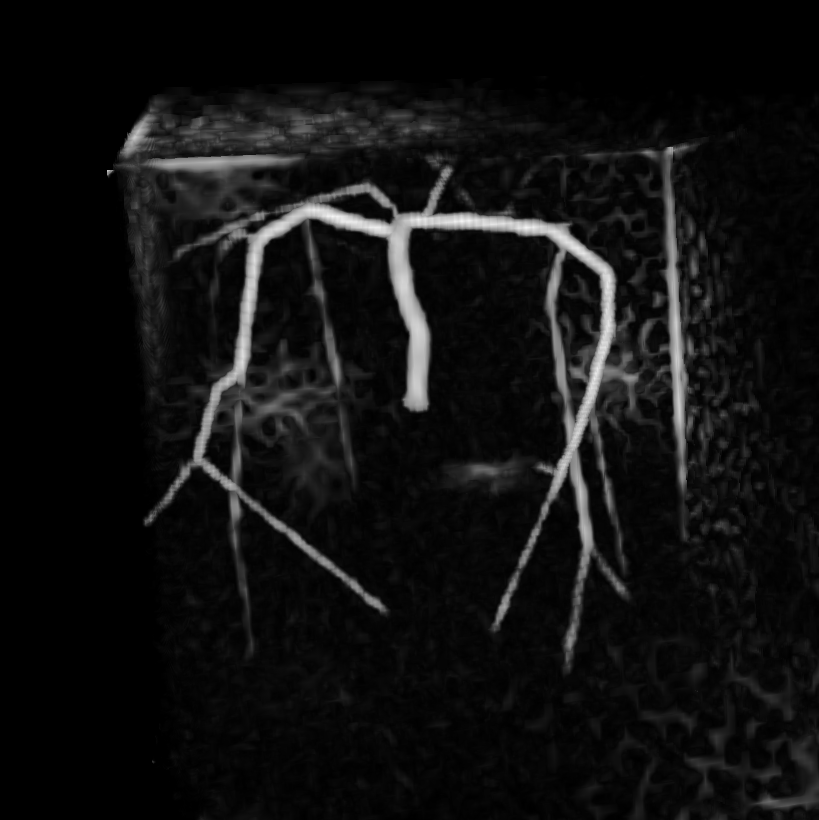
\includegraphics[clip = true, trim = 80 80 80 80,, height=25mm]{Images/Vascu_4_OOF_GM.png}
  \\
  % Meijering
  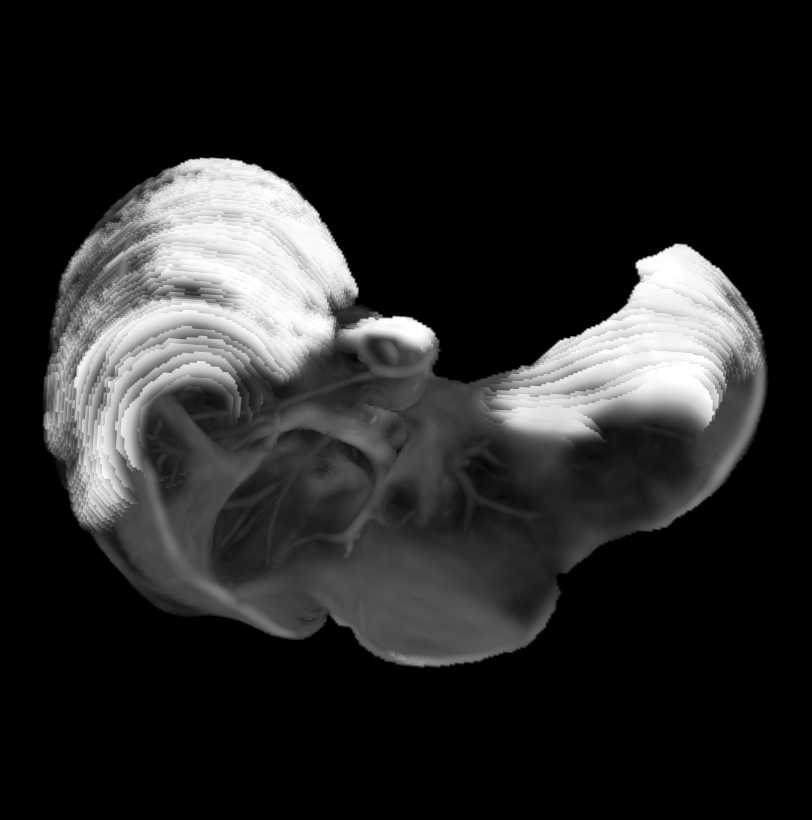
\includegraphics[clip = true, trim  =  10 150 10 150, height=25mm,width=36mm]{Images/Ircad_Meijering.png}
  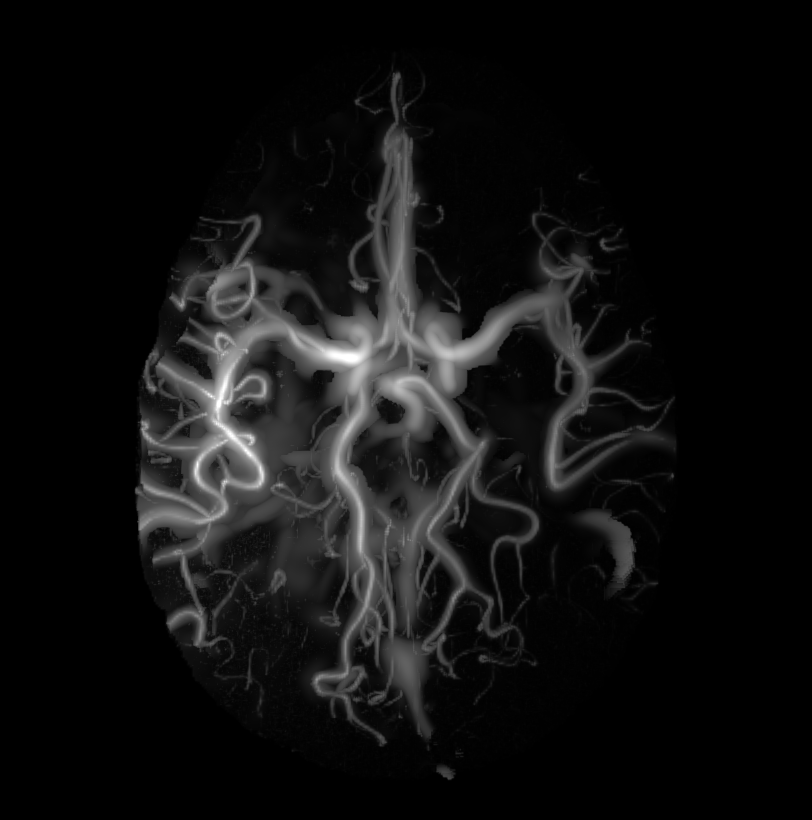
\includegraphics[clip = true, trim = 90 20 90 20, height=25mm,width=24mm]{Images/Bullitt_Meijering.png}
  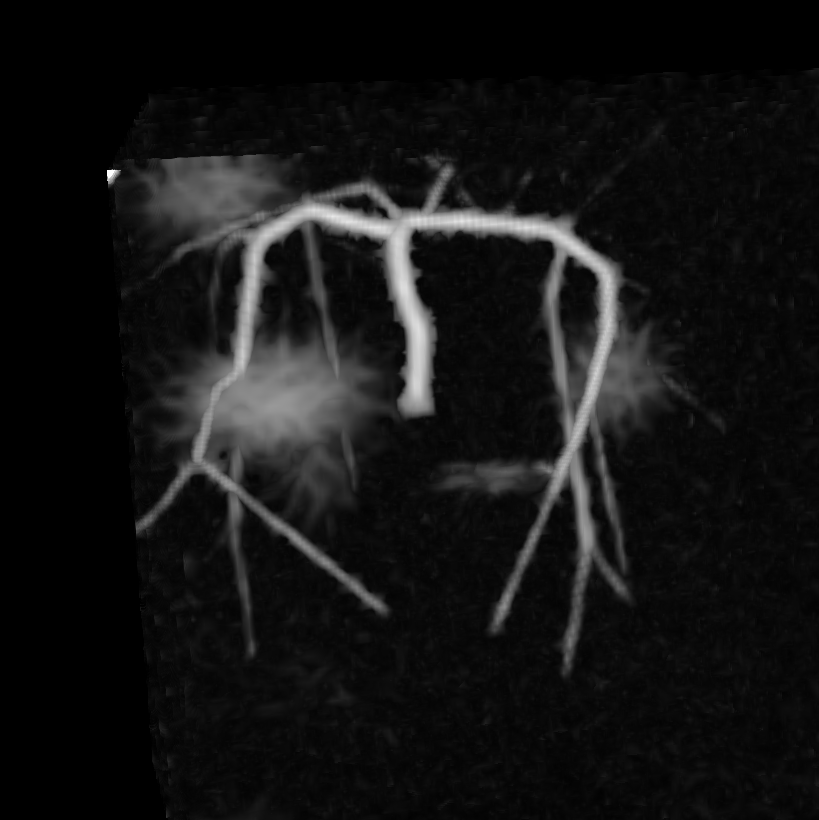
\includegraphics[clip = true, trim = 80 80 80 80, height=25mm]{Images/Vascu_4_Meijering.png}
  \\
  % RORPO
  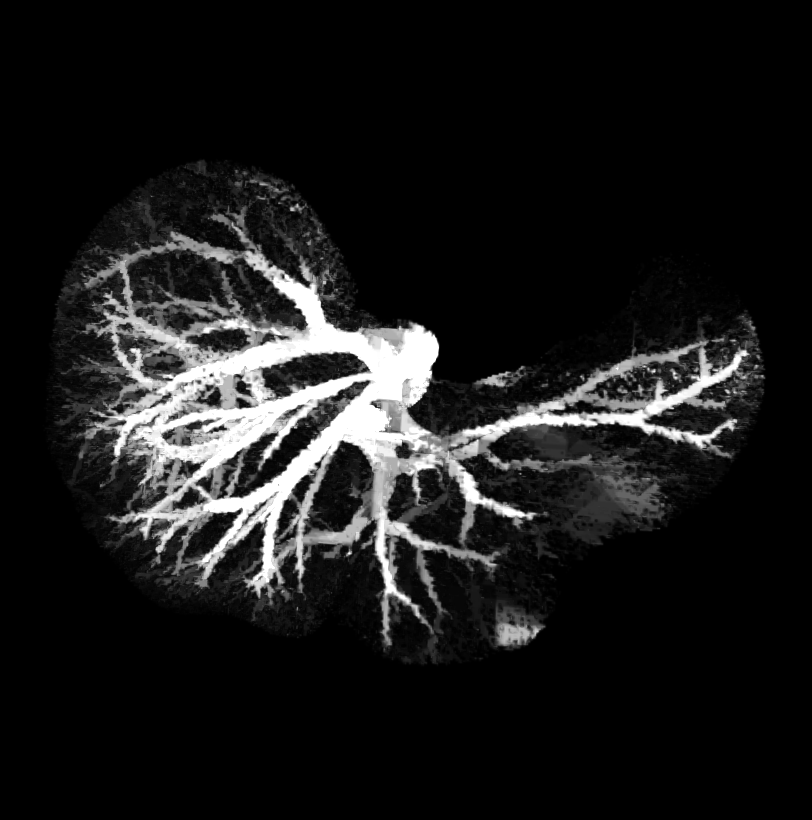
\includegraphics[clip = true, trim  =  10 150 10 150, height=25mm,width=36mm]{Images/Ircad_RORPO.png}
  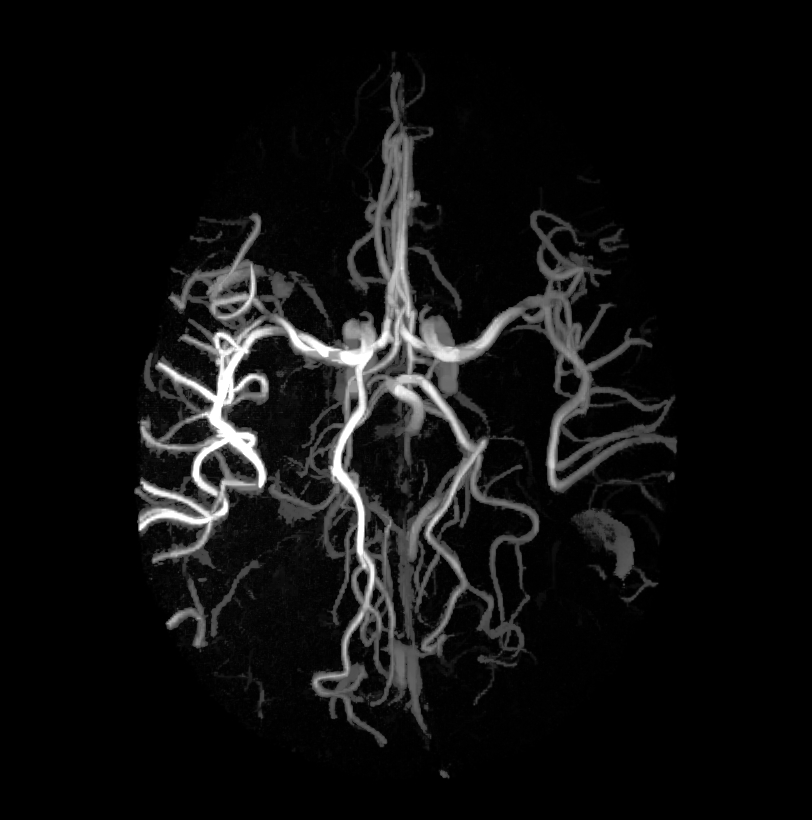
\includegraphics[clip = true, trim = 90 20 90 20, height=25mm,width=24mm]{Images/Bullitt_RORPO.png}
  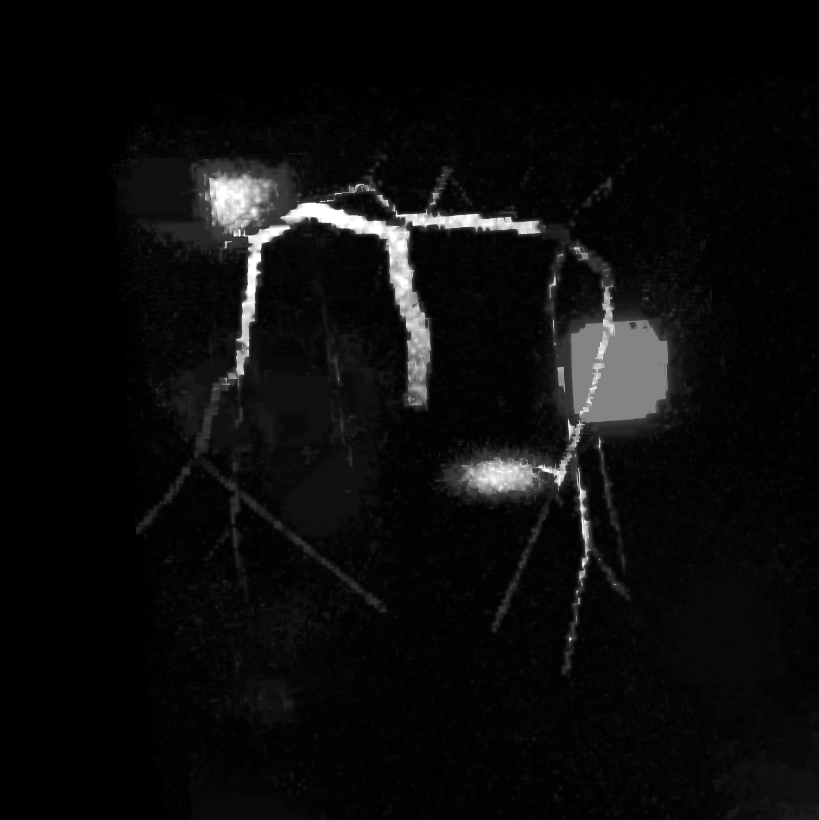
\includegraphics[clip = true, trim = 80 80 80 80, height=25mm]{Images/Vascu_4_RORPO.png}
  \\
  % Sato
  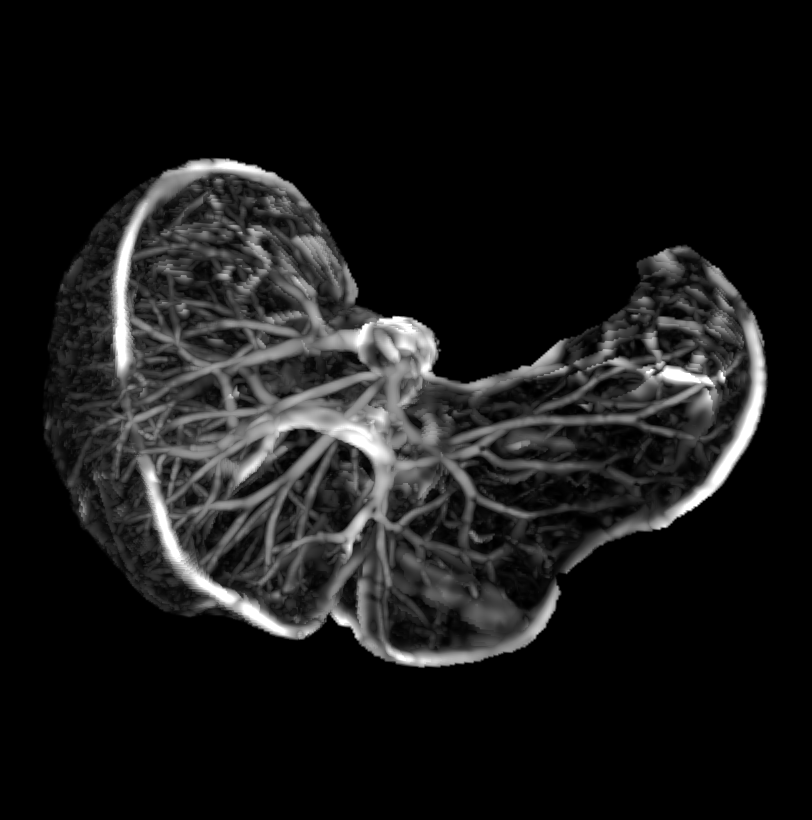
\includegraphics[clip = true, trim  =  10 150 10 150, height=25mm,width=36mm]{Images/Ircad_Sato.png}
  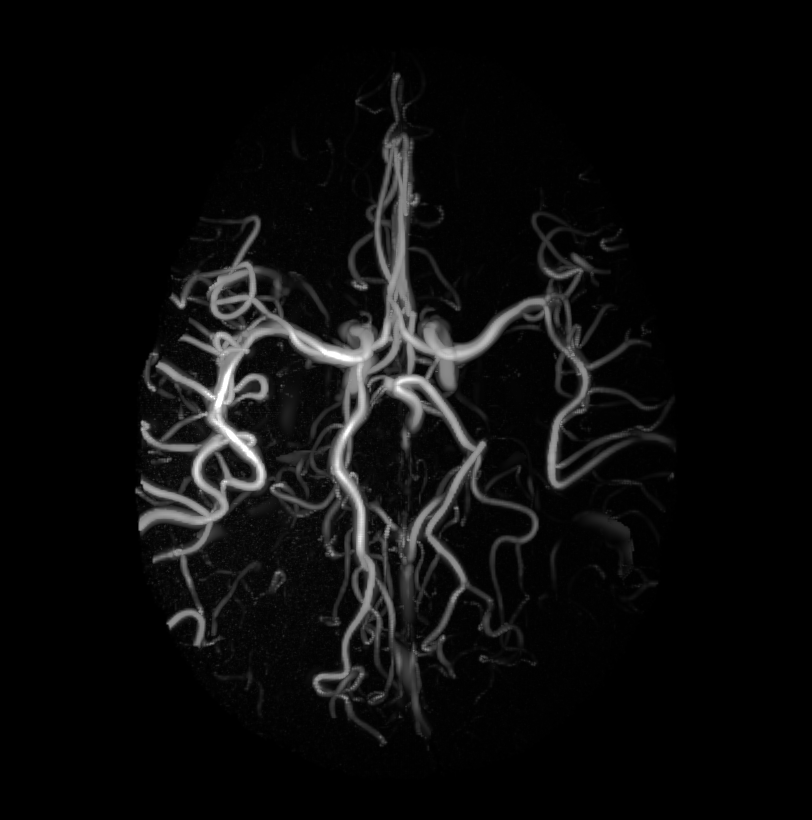
\includegraphics[clip = true, trim = 90 20 90 20,  height=25mm,width=24mm]{Images/Bullitt_Sato.png}
  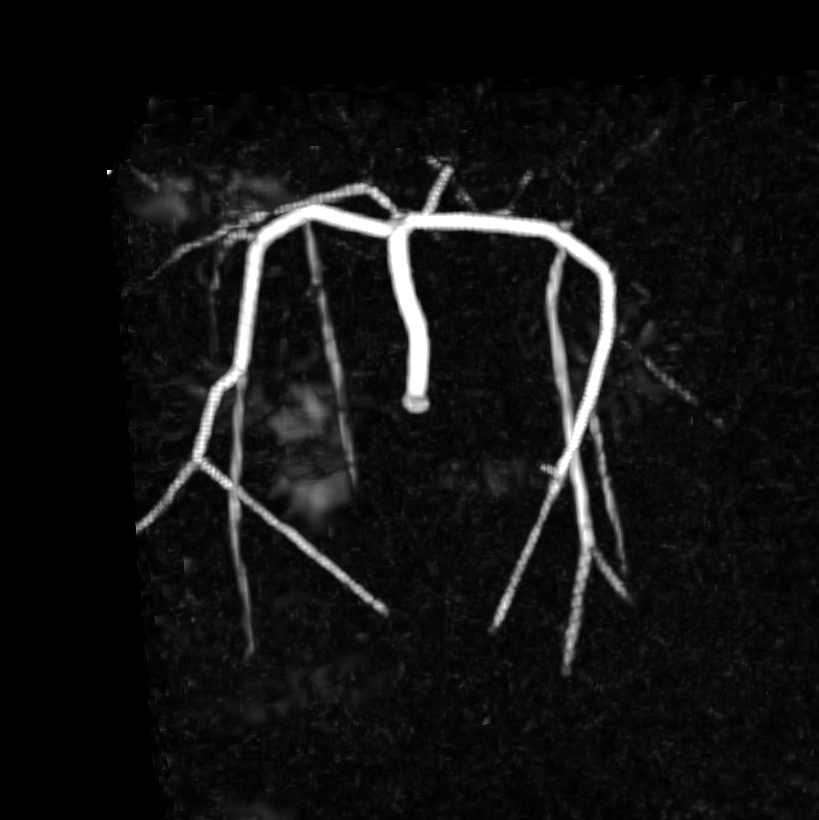
\includegraphics[clip = true, trim = 80 80 80 80, height=25mm]{Images/Vascu_4_Sato.png}
  \\
  % Zhang
  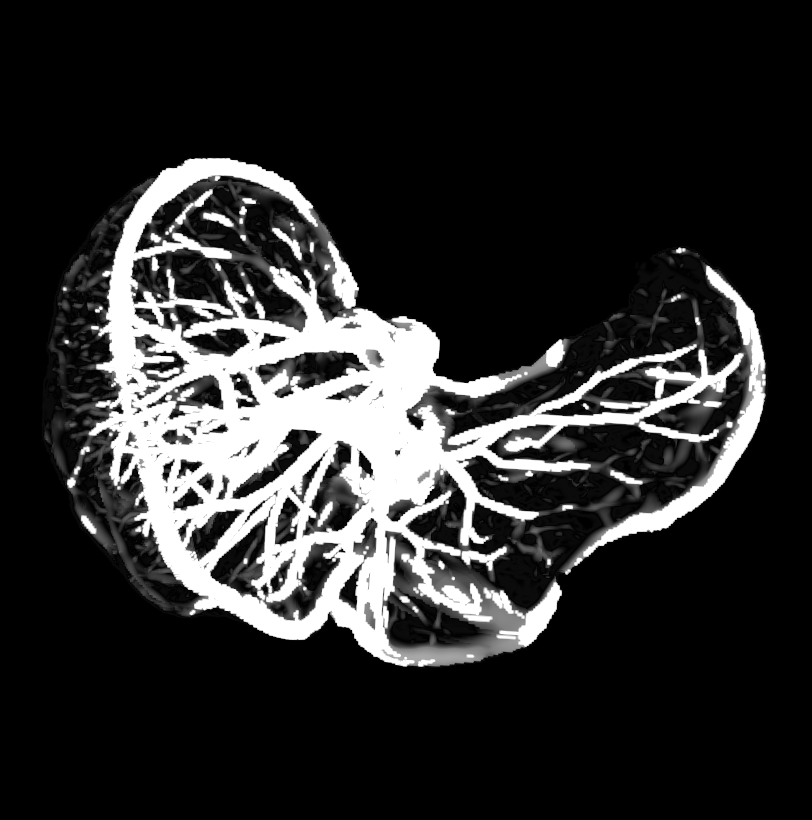
\includegraphics[clip = true, trim  =  10 150 10 150, height=25mm,width=36mm]{Images/Ircad_Zhang.png}
  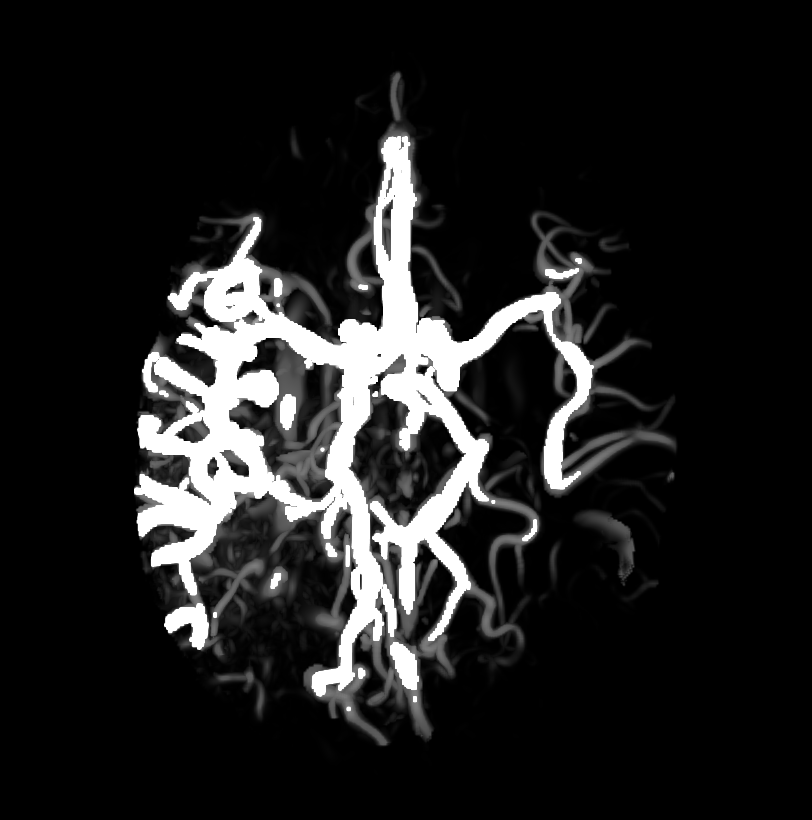
\includegraphics[clip = true, trim = 90 20 90 20, height=25mm,width=24mm]{Images/Bullitt_Zhang.png}
  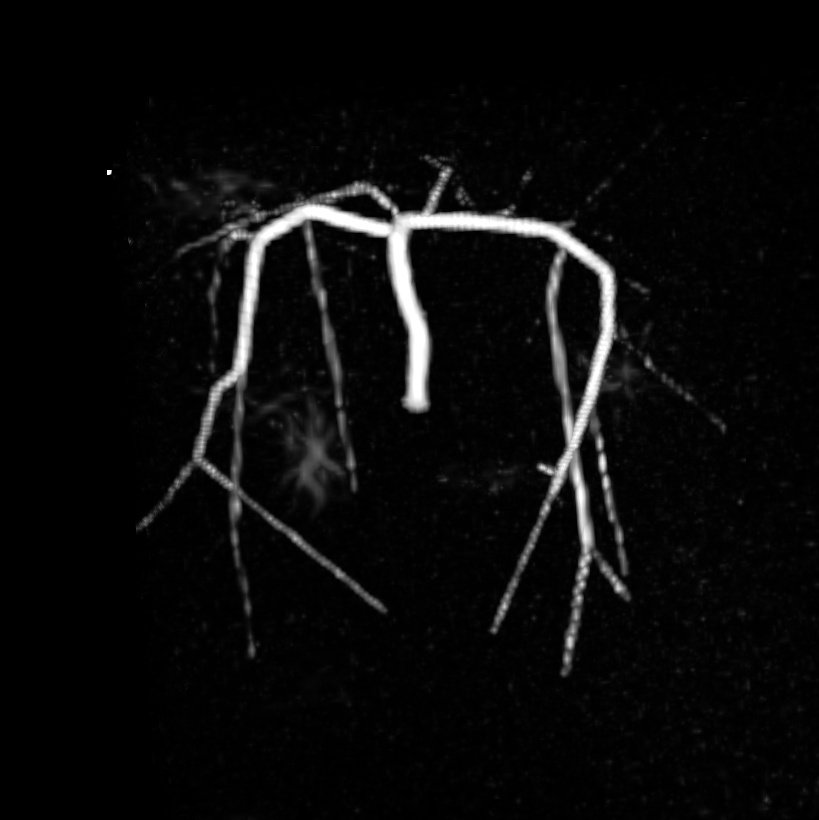
\includegraphics[clip = true, trim = 80 80 80 80, height=25mm]{Images/Vascu_4_Zhang.png}

  \caption{Illustration des résultats de filtrage optimisé pour l'Ircad (première colonne), Bullitt (seconde colonne) et  VascuSynth (troisième colonne).
  La première ligne correspond aux vérités terrains, suivies de la référence, Frangi, Jerman, OOF, Meijering, RORPO, Sato et Zhang.}
  \label{fig:quanlitative results}
\end{figure}

\paragraph{Ircad}

\begin{table}[!ht]
  \begin{center}
      \caption{Résultats quantitatifs (moyenne $\pm$ écart-type) dans le masque global \maskglobal sur le jeu de données de l'Ircad.}
      \label{Table:quantitative results Ircad}
      \begin{tabular}{lccc}
          \hline
          & MCC & Dice & PSNR \\ 
          \hline
          Référence	& $ 0.452 \pm 0.129	$ & $ 0.468 \pm	0.126 $ & $	9.352  \pm  1.247 $ \\
          Frangi	    & $ 0.355 \pm 0.075	$ & $ 0.392 \pm	0.074 $ & $	19.899 \pm 	1.624 $ \\
          Jerman	    & $ 0.382 \pm 0.060	$ & $ 0.415 \pm	0.059 $ & $	18.926 \pm 	1.186 $ \\
          Meijering   & $ 0.232 \pm 0.036	$ & $ 0.241 \pm	0.050 $ & $	19.079 \pm 	1.392 $ \\
          OOF	        & $ 0.277 \pm 0.049	$ & $ 0.316 \pm	0.055 $ & $	19.728 \pm 	1.575 $ \\
          RORPO	    & $ 0.475 \pm 0.073	$ & $ 0.477 \pm	0.076 $ & $	20.349 \pm 	1.687 $ \\
          Sato	    & $ 0.340 \pm 0.056	$ & $ 0.380 \pm	0.057 $ & $	19.915 \pm 	1.633 $ \\
          Zhang	    & $ 0.434 \pm 0.085	$ & $ 0.462 \pm	0.079 $ & $	20.274 \pm 	1.648 $ \\
    
          \hline
      \end{tabular}  
      \end{center}    
\end{table}


Globalement, le MCC et le Dice de tous les filtres appliqués sur les foies de l'Ircad sont faibles (inférieurs à 0.5). Ce résultat est attendu puisque nous avons réduit notre chaine de traitement au minimum. Cependant, ce résultat justifie quantitativement le fait qu'un filtre seul ne peut se substituer à une méthode de segmentation complète.

Qualitativement, tous les filtres excepté RORPO produisent des faux positifs sur les bordures du foie. Meijering semble produire les pires résultats en rehaussant à la fois fortement les bordures et le bruit dans les tissus. En comparaison, la référence, permet de bien récupérer les vaisseaux larges, mais la qualité des vaisseaux décroit, avec une augmentation des déconnections au fur et à mesure que les vaisseaux deviennent de plus en plus petit. 

Quantitativement, RORPO propose les meilleurs résultats avec un MCC de $0.475$. La base obtient le second meilleur MCC ($0.452$). Le fait qu'un simple seuillage produise de meilleurs résultats que la plupart des filtres sur ces images TM injectées peut paraitre étrange.

Cependant, ces résultats sont à pondérer par le fait que les moyens et petits vaisseaux manquent dans une proportion bien plus large dans la référence, par rapport aux filtres de rehaussement. En effet, tous les filtres ont des résultats supérieurs à la référence pour les moyens et petits vaisseaux.  

Zhang produit le troisième meilleur résultat (MCC = $0.434$), alors que OOF (MCC = $0.277$) et Meijering ($MCC = 0.231$) ont les performances les plus faibles. Les meilleurs filtres (RORPO et Zhang) obtiennent ces performances par des stratégies différentes. La précision de RORPO est élevée ($0.666$) avec une sensibilité moyenne ($0.379$). Au contraire, Zhang montre une sensitivité importante ($0.435$) contre une précision plus faible ($0.515$).

Nous rappelons que ces résultats sont basés sur le meilleur jeu de paramètres moyen sur le jeu de données entier. Le processus d'optimisation produit donc un compromis entre rehausser les vaisseaux et limiter l'intensité des voxels des structures qui ne sont pas des vaisseaux (tel que les bordures du foie). 

\paragraph{Bullitt}

\begin{table}[H]
  \begin{center}
      \caption{Résultats quantitatifs (moyenne $\pm$ écart-type) dans le masque global \maskglobal sur le jeu de données de Bullitt.}
      \label{Table:quantitative results Bullit}
  \begin{tabular}{lccc}
      \hline
          & MCC & Dice & PSNR \\ 
      \hline
      Référence	& $ 0.396 \pm 0.049 $ & $ 0.340 \pm 0.061 $ & $ 20.275 \pm	0.732 $ \\ 
      Frangi	    & $ 0.474 \pm 0.027 $ & $ 0.481 \pm 0.026 $ & $ 21.768 \pm	0.510 $ \\ 
      Jerman	    & $ 0.432 \pm 0.030 $ & $ 0.438 \pm 0.029 $ & $ 19.723 \pm	1.051 $ \\ 
      Meijering	& $ 0.349 \pm 0.040 $ & $ 0.354 \pm 0.043 $ & $ 21.905 \pm	0.463 $ \\ 
      OOF	        & $ 0.417 \pm 0.029 $ & $ 0.424 \pm 0.030 $ & $ 21.875 \pm	0.491 $ \\ 
      RORPO	    & $ 0.543 \pm 0.021 $ & $ 0.540 \pm 0.023 $ & $ 21.909 \pm	0.497 $ \\ 
      Sato	    & $ 0.475 \pm 0.026 $ & $ 0.473 \pm 0.028 $ & $ 21.799 \pm	0.466 $ \\ 
      Zhang	    & $ 0.423 \pm 0.037 $ & $ 0.431 \pm 0.037 $ & $ 21.261 \pm	0.847 $ \\ 

      \hline
  \end{tabular} 
\end{center}
\end{table}

Qualitativement, RORPO semble le mieux rehausser les vaisseaux avec peu de bruit. Cependant, les vaisseaux faiblement contrastés montrent des déconnections irrégulières typiques des filtres non extensifs. Quelques méthodes rehaussement le bruit dans les tissus du cerveau plus que d'autres tel que Jerman, Sato, Meijering et OOF. Cependant, Jerman et Sato présentent des profils de vaisseaux bien plus contrastés que le bruit. Le diamètre des vaisseaux est sur estimé par Jerman, Zhang, Meijering et dans une mesure plus réduite par OOF; Cela amène à la fusion de vaisseaux adjacents (voir fig \ref{fig:bifurcation_Bullitt}). Le rehaussement de Zhang est irrégulier avec certains vaisseaux très contrastés et d'autres faiblement contrastés. Zhang base son rehaussement sur un K-moyenne qui introduit un rehaussement dépendant de la classe associée aux pixels.

Nous attirons l'attention du lecteur sur le fait que nous n'avons pas observé d'artefacts liés au bord sur ce dataset puisque nous avons érodé le masque du cerveau de manière à exclure les veines non labélisées qui auraient biaisé nos métriques. 

Quantitativement, RORPO offre de meilleurs résultats par rapport aux autres filtres (MCC=$0.543$). Sato (MCC=$0.475$) et Frangi (MCC=$0.474$) arrivent respectivement en seconde et troisième position. Bien que présentant des MCC proches, le rappel de Frangi est meilleur que celui de Sato  ($0.469$ et $0.399$) mais avec un plus faible taux de précision ($0.498$ vs. $0.585$). Jerman (MCC=$0.432$), Zhang (MCC=$0.424$) et OOF (MCC=$0.417$) montrent des résultats supérieurs à la base de référence (MCC=$0.396$) tandis que Meijering produit un fort taux de faux positif qui pénalise le MCC ($0.349$).



\paragraph{VascuSynth}


\begin{table}[H]
    \begin{center}
    \caption{Résultats quantitatifs (moyenne $\pm$ écart-type) dans le masque global \maskglobal sur les jeux de données de VascuSynth.}
    \label{Table:quantitative results Vascusynth}
    \resizebox{\textwidth}{!}{
    \begin{tabular}{l|ccc|ccc|ccc}
    \hline
          & \multicolumn{3}{c|}{MCC} & \multicolumn{3}{c|}{Dice} & \multicolumn{3}{c}{PSNR} \\
          & $\sigma = 2$ & $\sigma = 4$ & $\sigma = 6$ & $\sigma = 2$ & $\sigma = 4$ & $\sigma = 6$ & $\sigma = 2$ & $\sigma = 4$ & $\sigma = 6$\\
         \hline
         Baseline	& $ 0.184 \pm 0.136 $  & $ 0.143 \pm 0.116 $ & $ 0.106 \pm	0.089 $ & $	0.162 \pm 0.134 $ & $ 0.122 \pm 0.114 $ & $	0.089 \pm  0.087 $ & $  9.411 \pm   0.231 $ & $  9.397  \pm 0.230 $ & $  9.374  \pm	0.229 $ \\
         Frangi	    & $ 0.634 \pm 0.051 $  & $ 0.577 \pm 0.070 $ & $ 0.500 \pm	0.081 $ & $	0.621 \pm 0.049 $ & $ 0.572 \pm 0.074 $ & $	0.485 \pm  0.091 $ & $ 26.274 \pm 	2.813 $ & $	26.496	\pm 2.872 $	& $ 26.692	\pm 2.856 $ \\
         Jerman	    & $ 0.611 \pm 0.064 $  & $ 0.565 \pm 0.049 $ & $ 0.501 \pm	0.048 $ & $	0.603 \pm 0.065 $ & $ 0.549 \pm 0.046 $ & $	0.464 \pm  0.048 $ & $ 26.774 \pm 	1.296 $ & $	21.758	\pm 0.399 $	& $ 21.831	\pm 0.489 $ \\
         OOF	    & $ 0.627 \pm 0.061 $  & $ 0.496 \pm 0.065 $ & $ 0.449 \pm	0.069 $ & $	0.530 \pm 0.060 $ & $ 0.476 \pm 0.063 $ & $	0.419 \pm  0.067 $ & $ 26.324 \pm 	1.802 $ & $	24.594	\pm 1.329 $	& $ 22.983	\pm 1.072 $ \\
         Meijering	& $ 0.538 \pm 0.061 $  & $ 0.603 \pm 0.059 $ & $ 0.565 \pm	0.060 $ & $	0.619 \pm 0.064 $ & $ 0.599 \pm 0.061 $ & $	0.564 \pm  0.059 $ & $ 26.586 \pm 	2.331 $ & $	25.902	\pm 1.889 $	& $ 24.821	\pm 1.395 $ \\
         RORPO	    & $ 0.587 \pm 0.155 $  & $ 0.517 \pm 0.119 $ & $ 0.366 \pm	0.123 $ & $	0.554 \pm 0.157 $ & $ 0.476 \pm 0.117 $ & $	0.325 \pm  0.113 $ & $ 23.236 \pm 	2.472 $ & $	20.672	\pm 1.689 $	& $ 18.372	\pm 1.571 $ \\
         Sato	    & $ 0.618 \pm 0.046 $  & $ 0.559 \pm 0.058 $ & $ 0.488 \pm	0.052 $ & $	0.596 \pm 0.044 $ & $ 0.548 \pm 0.058 $ & $	0.464 \pm  0.050 $ & $ 26.602 \pm 	2.539 $ & $	26.241	\pm 1.803 $	& $ 24.801	\pm 1.285 $ \\
         Zhang	    & $ 0.553 \pm 0.052 $  & $ 0.523 \pm 0.051 $ & $ 0.481 \pm	0.065 $ & $	0.531 \pm 0.051 $ & $ 0.498 \pm 0.049 $ & $	0.474 \pm  0.067 $ & $ 26.221 \pm 	2.805 $ & $	26.360	\pm 2.826 $	& $ 26.543	\pm 2.845 $ \\
   
    \end{tabular} }
    \end{center}
\end{table}

Qualitativement, Meijering, Sato et Jerman produisent les meilleurs résultats. Cependant, Meijering a tendance à rehausser le bruit au voisinage des vaisseaux donnant à leur contour un aspect irrégulier. Jerman a un rehaussement des vaisseaux de bonne qualité, mais rehausse aussi une bonne partie du bruit. Frangi, Zhang et Sato semblent être les meilleures méthodes pour filtrer le bruit ricien. 

Dans ce jeu de données, RORPO est plus sensible au bruit. Plus le bruit est important, plus les artefacts en forme de blob sont rehaussés. Ce comportement était en partie attendu puisque nous n'avons pas utilisé le paramètre de dilatation de RORPO (qui gère les déconnections liées au bruit) en le laissant à 0. Ce choix a été motivé par le fait que ce paramètre ne peut pas être optimisé séparément des paramètres d'échelles. Dans des applications réelles avec un fort niveau de bruit, l'étude de ce paramètre est indispensable. 
Comme le jeu de données VascuSynth ne présente pas de bordures d'organes où d'artefacts similaires, l'éventualité d'un faux rehaussement lié à ces artefacts est limitée comparé aux jeux de données rééls, excepté pour OOF qui rehausse les bordures de l'image assimilées à des plans. La mesure utilisée pour OOF distingue en effet mal les structures planaires des structures tubulaires. Une autre mesure de tubularité tel que la mesure de Frangi pourrait être utilisée pour éviter ce problème. Etrangement, quand le bruit n'est pas bien filtré, les filtres de rehaussements ont tendance à introduire de fausses structures tubulaires non présentes dans l'image d'origine (Fig. \ref{fig:noisy_tubes}).

\begin{figure}[H]
  \centering
  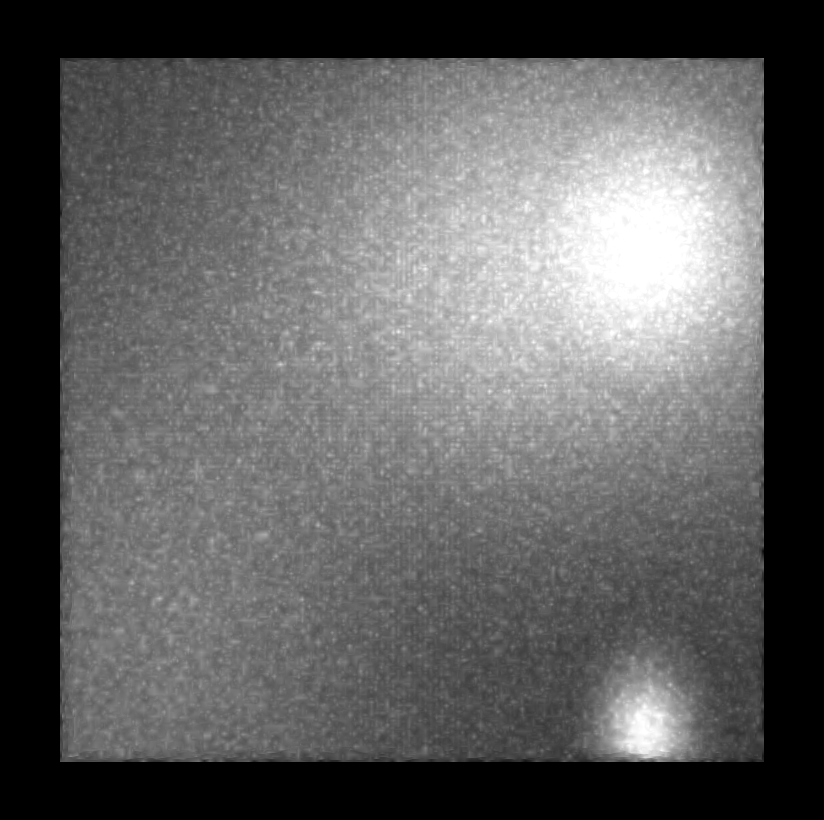
\includegraphics[height=4cm]{Images/vascu_noise.png}
  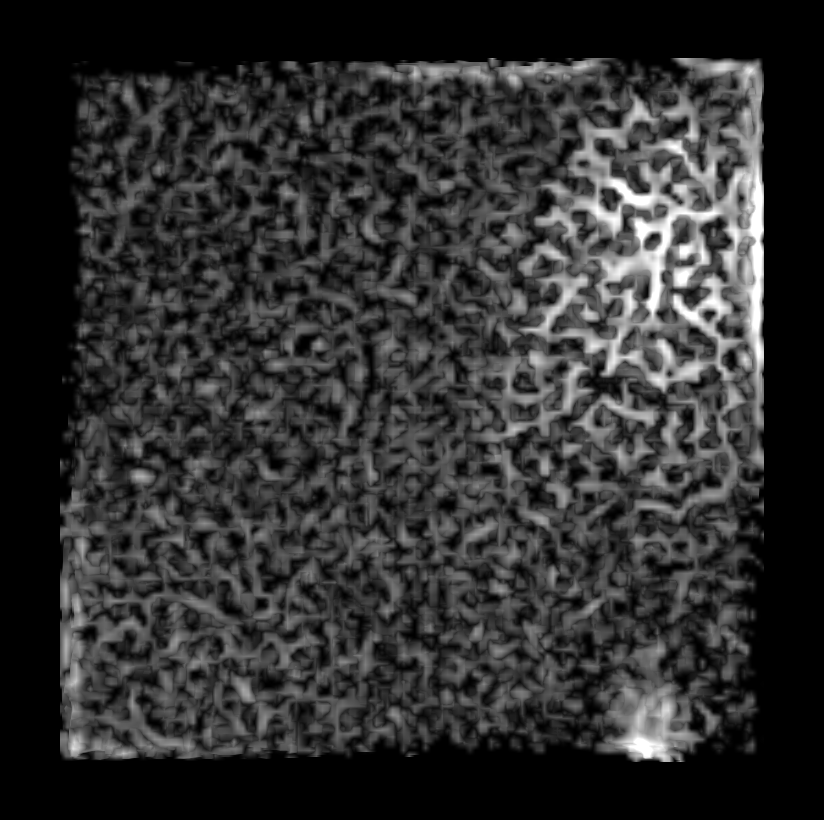
\includegraphics[height=4cm]{Images/vascu_noise_OOF.png}
  \caption{Bruit de fond de Vascusynth $\sigma=4$ et bruit de fond après filtrage par OOF.}
  \label{fig:noisy_tubes}
\end{figure}

Quantitativement, Frangi donne les meilleurs résultats $\sigma=2$ avec un MCC de $0.634$ et Meijering pour les deux autres niveaux atteignant un MCC de $0.603$ pour $\sigma=4$ et $0.565$ pour $\sigma=6$. Ces bonnes performances de Meijering sont expliqués par le fait que la géométrie des vaisseaux de VascuSynth correspond aux hypothèses du modèle de Meijering (vaisseaux droits, et de rayon constant). Sato obtient le troisième meilleurs résultats pour le niveau de bruit $\sigma=2$ (MCC=$0.618$) tandis que Jerman exhibe de meilleurs résultats pour des niveaux de bruits supérieurs (MCC = $0.565$ pour $\sigma=4$ and MCC=$0.501$ pour $\sigma = 6$). Peu importe les cas, les deux filtres donnent des résultats similaires, puisque leur sensibilité est similaire, indépendamment du niveau de bruit. La différence entre les deux filtres s'explique au niveau de la précision : pour des niveaux de bruit élevés (e.g. $\sigma=4$), Jerman présente une plus grande précision (MCC = $0.717$ vs $0.661$) tandis que Sato montre une précision supérieure pour les faibles niveaux de bruit (MCC = $0.810$ vs $0.689$). En général, Frangi est la méthode qui ignore le mieux le bruit pour des niveaux de bruit haut avec un PSNR de $26.496$ et $26.692$ pour $\sigma=4$ et $\sigma=6$, respectivement. Les résultats de la référence sont très mauvais à cause de la présence d'artefacts de haute intensité et d'un fond non homogène dans les données de VascuSynth. Ce comportement est une motivation supplémentaire pour l'usage de filtres de rehaussement pour des applications avec un contexte similaire. Globalement, RORPO produit les moins bons résultats sur VascuSynth alors que Zhang reste relativement stable, peu importe le niveau de bruit choisi.

\subsection{Voisinage des vaisseaux}
Les résultats quantitatifs des sept filtres sont présentés dans les tables \ref{tab:VesselssizeIrcad} -- \ref{tab:Vessels size VascuSynth} pour les jeux de données de l'Ircad, Bullitt et VascuSynth 

\paragraph{Ircad}

\begin{table}[H]
  \begin{center}
  \caption{Résultats quantitatifs (moyenne $\pm$ écart-type) par catégorie de tailles de vaisseaux pour l'Ircad.}
  \label{tab:VesselssizeIrcad}
  \resizebox{\textwidth}{!}{    
  \begin{tabular}{lccc|ccc}
                \hline
                & \multicolumn{3}{c}{Voisinage}                                   & \multicolumn{3}{c}{Larges}                                            \\
                \hline
                & MCC  &  Dice & PSNR & MCC  &  Dice  &  PSNR  \\
                Baseline	& $ 0.491 \pm	0.118 $ & $	0.527 \pm 0.110 $ & $ 13.110 \pm 1.795 $ & $ 0.552 \pm 	0.130 $ & $	0.597 \pm 0.136 $ & $ 20.938 \pm 2.637 $ \\
                Frangi  	& $ 0.535 \pm	0.073 $ & $	0.581 \pm 0.065 $ & $ 19.989 \pm 1.653 $ & $ 0.580 \pm 	0.072 $ & $	0.627 \pm 0.087 $ & $ 22.189 \pm 1.867 $ \\
                Jerman	& $ 0.501 \pm	0.054 $ & $	0.521 \pm 0.060 $ & $ 21.464 \pm 1.757 $ & $ 0.480 \pm 	0.065 $ & $	0.496 \pm 0.083 $ & $ 24.119 \pm 1.972 $ \\
                Meijering	& $ 0.451 \pm	0.061 $ & $	0.522 \pm 0.049 $ & $ 20.091 \pm 1.646 $ & $ 0.545 \pm 	0.055 $ & $	0.669 \pm 0.044 $ & $ 22.407 \pm 1.850 $ \\
                OOF	    & $ 0.498 \pm	0.063 $ & $	0.556 \pm 0.051 $ & $ 19.912 \pm 1.642 $ & $ 0.513 \pm 	0.060 $ & $	0.574 \pm 0.067 $ & $ 22.056 \pm 1.850 $ \\
                RORPO	    & $ 0.491 \pm	0.066 $ & $	0.501 \pm 0.075 $ & $ 20.463 \pm 1.765 $ & $ 0.491 \pm 	0.069 $ & $	0.504 \pm 0.080 $ & $ 22.580 \pm 1.948 $ \\
                Sato	    & $ 0.508 \pm	0.054 $ & $	0.542 \pm 0.057 $ & $ 19.996 \pm 1.679 $ & $ 0.512 \pm 	0.067 $ & $	0.548 \pm 0.086 $ & $ 22.130 \pm 1.861 $ \\
                Zhang	    & $ 0.535 \pm	0.064 $ & $	0.551 \pm 0.074 $ & $ 20.940 \pm 1.857 $ & $ 0.541 \pm 	0.078 $ & $	0.561 \pm 0.101 $ & $ 23.199 \pm 2.032 $ \\
      
                \hline
                & \multicolumn{3}{c}{Moyens}                                         & \multicolumn{3}{c}{Petits}                                            \\
                \hline
                & MCC  &  Dice & PSNR & MCC  &  Dice  &  PSNR  \\
                Baseline	& $ 0.509 \pm 0.121 $ & $	0.557 \pm 0.117 $ & $ 21.250 \pm 2.989 $ & $ 0.391 \pm	0.103 $ & $	0.424 \pm 0.097 $ & $ 18.687 \pm 2.209 $ \\
                Frangi    & $ 0.619 \pm 0.115 $ & $	0.660 \pm 0.113 $ & $ 27.387 \pm 2.554 $ & $ 0.460 \pm	0.123 $ & $	0.506 \pm 0.118 $ & $ 26.624 \pm 2.232 $ \\
                Jerman    & $ 0.604 \pm 0.095 $ & $	0.622 \pm 0.110 $ & $ 30.111 \pm 3.155 $ & $ 0.502 \pm	0.093 $ & $	0.525 \pm 0.104 $ & $ 27.991 \pm 2.120 $ \\
                Meijering & $ 0.542 \pm 0.085 $ & $	0.602 \pm 0.082 $ & $ 27.432 \pm 2.474 $ & $ 0.419 \pm	0.088 $ & $	0.462 \pm 0.077 $ & $ 26.723 \pm 2.187 $ \\
                OOF	    & $ 0.642 \pm 0.097 $ & $	0.681 \pm 0.097 $ & $ 27.334 \pm 2.467 $ & $ 0.514 \pm	0.103 $ & $	0.559 \pm 0.096 $ & $ 26.692 \pm 2.251 $ \\
                RORPO	    & $ 0.547 \pm 0.102 $ & $	0.573 \pm 0.115 $ & $ 28.138 \pm 2.637 $ & $ 0.417 \pm	0.093 $ & $	0.435 \pm 0.104 $ & $ 27.157 \pm 2.354 $ \\
                Sato	    & $ 0.602 \pm 0.096 $ & $	0.629 \pm 0.105 $ & $ 27.437 \pm 2.548 $ & $ 0.488 \pm	0.092 $ & $	0.522 \pm 0.091 $ & $ 26.777 \pm 2.277 $ \\
                Zhang	    & $ 0.602 \pm 0.110 $ & $	0.619 \pm 0.126 $ & $ 28.808 \pm 3.119 $ & $ 0.481 \pm	0.110 $ & $	0.497 \pm 0.124 $ & $ 27.471 \pm 2.311 $ \\        
      \hline
      \end{tabular}

  }
  \end{center}
\end{table}


Tous les filtres hessiens et OOF ont des performances qui augmentent significativement quand ils sont calculés dans \maskvessel, puisque les artefacts éloignés des vaisseaux sont ignorés par le masque \maskvessel. Dans ce masque, Frangi et Zhang sont tous les deux les meilleurs filtres (MCC=$0.535$). En étudiant les performances des filtres en fonction de la taille des vaisseaux rehaussés (\maskvesselLarge,\maskvesselMedium,\maskvesselSmall), on observe que Frangi est capable de bien rehausser les vaisseaux larges (MCC=$0.580$) et moyens (MCC= $0.619$), mais ses performances baissent pour les petits vaisseaux (MCC=$0.460$). À l'inverse, OOF et Jerman rehaussent correctement les petits vaisseaux (MCC=$0.514$ et MCC=$0.502$) mais avec des performances réduites sur les gros vaisseaux (MCC=$0.513$ et MCC=$0.480$)   

\paragraph{Bullitt}

\begin{table}[H]
  \begin{center}
  \label{tab:Vessels size Bullitt}
  \caption{Résultats quantitatifs (moyenne $\pm$ écart-type) par catégorie de tailles de vaisseaux pour Bullitts.}
  
  \begin{tabular}{lccc}
            \hline
            & \multicolumn{3}{c}{Voisinage}                  \\
            \hline
            & MCC & Dice & PSNR  \\
            Baseline	    & $ 0.371 \pm 0.038 $ & $ 0.341 \pm 0.062 $ & $ 22.291 \pm	0.513 $ \\
            Frangi	    & $ 0.415 \pm 0.028 $ & $ 0.506 \pm 0.026 $ & $ 21.641 \pm	0.517 $ \\
            Jerman	    & $ 0.377 \pm 0.037 $ & $ 0.466 \pm 0.029 $ & $ 21.990 \pm	0.687 $ \\
            Meijering	    & $ 0.288 \pm 0.041 $ & $ 0.412 \pm 0.045 $ & $ 22.076 \pm	0.509 $ \\ 
            OOF	        & $ 0.353 \pm 0.026 $ & $ 0.456 \pm 0.032 $ & $ 21.771 \pm	0.506 $ \\
            RORPO	        & $ 0.506 \pm 0.022 $ & $ 0.556 \pm 0.025 $ & $ 21.784 \pm	0.506 $ \\
            Sato	        & $ 0.435 \pm 0.027 $ & $ 0.491 \pm 0.029 $ & $ 21.698 \pm	0.478 $ \\
            Zhang	        & $ 0.348 \pm 0.029 $ & $ 0.460 \pm 0.026 $ & $ 21.430 \pm	0.553 $ \\
      
            \hline
            & \multicolumn{3}{c}{Moyens}                         \\
            \hline    
            & MCC & Dice & PSNR  \\
            Baseline	& $ 0.542 \pm 0.129 $ & $ 0.555 \pm 0.163 $ & $ 33.836 \pm	2.891 $ \\
            Frangi	& $ 0.605 \pm 0.034 $ & $ 0.684 \pm 0.034 $ & $ 33.262 \pm	2.827 $ \\
            Jerman	& $ 0.580 \pm 0.048 $ & $ 0.660 \pm 0.055 $ & $ 34.066 \pm	3.226 $ \\
            Meijering	& $ 0.402 \pm 0.054 $ & $ 0.521 \pm 0.067 $ & $ 34.034 \pm	2.820 $ \\
            OOF	    & $ 0.620 \pm 0.049 $ & $ 0.690 \pm 0.044 $ & $ 33.621 \pm	2.971 $ \\
            RORPO	    & $ 0.647 \pm 0.047 $ & $ 0.712 \pm 0.047 $ & $ 33.370 \pm	2.882 $ \\
            Sato	    & $ 0.594 \pm 0.064 $ & $ 0.663 \pm 0.088 $ & $ 33.072 \pm	2.928 $ \\
            Zhang	    & $ 0.577 \pm 0.074 $ & $ 0.655 \pm 0.101 $ & $ 33.789 \pm	2.790 $ \\
            \hline
            & \multicolumn{3}{c}{Petits}                          \\
            \hline
            & MCC & Dice & PSNR  \\
            Baseline	    & $ 0.358 \pm 0.038 $ & $ 0.315 \pm 0.057 $ & $ 22.771 \pm	0.591 $ \\
            Frangi	    & $ 0.419 \pm 0.024 $ & $ 0.491 \pm 0.026 $ & $ 22.153 \pm	0.609 $ \\
            Jerman  	    & $ 0.376 \pm 0.031 $ & $ 0.445 \pm 0.030 $ & $ 22.352 \pm	0.863 $ \\
            Meijering	    & $ 0.287 \pm 0.040 $ & $ 0.382 \pm 0.044 $ & $ 22.549 \pm	0.593 $ \\
            OOF	        & $ 0.353 \pm 0.025 $ & $ 0.436 \pm 0.038 $ & $ 22.275 \pm	0.586 $ \\
            RORPO	        & $ 0.510 \pm 0.023 $ & $ 0.544 \pm 0.027 $ & $ 22.307 \pm	0.590 $ \\
            Sato	        & $ 0.436 \pm 0.024 $ & $ 0.473 \pm 0.031 $ & $ 22.236 \pm	0.572 $ \\
            Zhang	        & $ 0.349 \pm 0.022 $ & $ 0.440 \pm 0.023 $ & $ 21.861 \pm	0.680 $ \\
  \hline
  \end{tabular}
  \end{center}
\end{table}

Localement, les résultats pour \maskglobal et \maskvessel sont similaires puisqu'il ne contient quasiment pas de structures autres que les vaisseaux. Dans ce contexte, RORPO est toujours le meilleur filtre suivi de Sato et Frangi.

\paragraph{VascuSynth}

\begin{table}[H]
  \begin{centering}
  \caption{Résultats quantitatifs (moyenne $\pm$ écart-type) par catégorie de tailles de vaisseaux pour VascuSynth ($\sigma=2$).}
  \label{tab:Vessels size VascuSynth}
  \resizebox{\textwidth}{!}{
  \begin{tabular}{lccc|ccc}
            \hline
            & \multicolumn{3}{c}{Voisinage}  & \multicolumn{3}{c}{Larges}                           \\
            \hline
            & MCC   & Dice & PSNR & MCC & Dice & PSNR  \\
            Baseline	    & $ 0.392 \pm 0.145 $ & $ 0.340 \pm	0.172 $ & $	25.198 \pm	3.109 $ & $ 0.515 \pm 0.293 $ & $ 0.491 \pm 0.307 $ & $ 30.738 \pm 1.278 $ \\
            Frangi	    & $ 0.700 \pm 0.037 $ & $ 0.688 \pm	0.044 $ & $	26.275 \pm	2.814 $ & $ 0.757 \pm 0.022 $ & $ 0.747 \pm 0.025 $ & $ 32.939 \pm 0.934 $ \\
            Jerman	    & $ 0.710 \pm 0.055 $ & $ 0.702 \pm	0.067 $ & $	29.880 \pm	3.007 $ & $ 0.735 \pm 0.027 $ & $ 0.722 \pm 0.031 $ & $ 36.312 \pm 0.973 $ \\
            Meijering	    & $ 0.725 \pm 0.034 $ & $ 0.753 \pm	0.035 $ & $	27.305 \pm	2.969 $ & $ 0.818 \pm 0.028 $ & $ 0.834 \pm 0.028 $ & $ 34.217 \pm 0.978 $ \\
            OOF	        & $ 0.648 \pm 0.043 $ & $ 0.624 \pm	0.053 $ & $	28.275 \pm	2.968 $ & $ 0.714 \pm 0.025 $ & $ 0.696 \pm 0.029 $ & $ 35.068 \pm 0.980 $ \\
            RORPO	        & $ 0.639 \pm 0.082 $ & $ 0.619 \pm	0.096 $ & $	29.406 \pm	3.407 $ & $ 0.713 \pm 0.165 $ & $ 0.694 \pm 0.197 $ & $ 37.049 \pm 1.574 $ \\
            Sato	        & $ 0.661 \pm 0.034 $ & $ 0.642 \pm	0.042 $ & $	26.938 \pm	2.867 $ & $ 0.731 \pm 0.024 $ & $ 0.719 \pm 0.028 $ & $ 33.699 \pm 0.945 $ \\
            Zhang	        & $ 0.624 \pm 0.042 $ & $ 0.594 \pm	0.053 $ & $	26.225 \pm	2.809 $ & $ 0.713 \pm 0.041 $ & $ 0.696 \pm 0.050 $ & $ 32.893 \pm 0.936 $ \\
      
            \hline
            & \multicolumn{3}{c}{Moyens}                         & \multicolumn{3}{c}{Petits}                           \\
            \hline
            & MCC  & Dice & PSNR & MCC & Dice & PSNR  \\
            Baseline	    & $ 0.415 \pm 0.176 $ & $ 0.355 \pm 0.202 $ & $	26.699 \pm 1.974 $ & $	0.284 \pm 0.125 $ & $ 0.218 \pm 0.129 $ & $ 27.954 \pm 3.858 $ \\
            Frangi	    & $ 0.715 \pm 0.035 $ & $ 0.698 \pm 0.041 $ & $	28.986 \pm 2.026 $ & $	0.683 \pm 0.056 $ & $ 0.657 \pm 0.069 $ & $ 30.328 \pm 3.627 $ \\
            Jerman	    & $ 0.708 \pm 0.047 $ & $ 0.691 \pm 0.057 $ & $	32.360 \pm 2.236 $ & $	0.730 \pm 0.073 $ & $ 0.719 \pm 0.090 $ & $ 34.315 \pm 4.028 $ \\
            OOF	        & $ 0.768 \pm 0.031 $ & $ 0.785 \pm 0.031 $ & $	30.159 \pm 2.141 $ & $	0.660 \pm 0.072 $ & $ 0.652 \pm 0.086 $ & $ 31.054 \pm 3.723 $ \\
            Meijering	    & $ 0.672 \pm 0.040 $ & $ 0.646 \pm 0.049 $ & $	31.016 \pm 2.152 $ & $	0.615 \pm 0.071 $ & $ 0.572 \pm 0.091 $ & $ 32.202 \pm 3.802 $ \\
            RORPO	        & $ 0.670 \pm 0.087 $ & $ 0.647 \pm 0.101 $ & $	32.281 \pm 2.506 $ & $	0.566 \pm 0.108 $ & $ 0.523 \pm 0.118 $ & $ 32.660 \pm 3.946 $ \\
            Sato	        & $ 0.675 \pm 0.035 $ & $ 0.649 \pm 0.042 $ & $	29.659 \pm 2.078 $ & $	0.647 \pm 0.047 $ & $ 0.615 \pm 0.059 $ & $ 30.939 \pm 3.674 $ \\
            Zhang	        & $ 0.648 \pm 0.044 $ & $ 0.616 \pm 0.054 $ & $	28.936 \pm 2.024 $ & $	0.580 \pm 0.054 $ & $ 0.528 \pm 0.071 $ & $ 30.278 \pm 3.618 $ \\
  \hline
  \end{tabular}
  }
  \end{centering} 
\end{table}

Globalement, le rehaussement des vaisseaux est le mieux réalisé par Frangi, à l'exception du plus faible niveau de bruit où Meijering obtient les meilleurs résultats. Une analyse plus fine des résultats par tailles montrent que Meijering et Jerman obtient de meilleurs résultats que Frangi sur les vaisseaux moyen et petits pour de faibles niveaux de bruit.  Dans les autres cas, Frangi produit de meilleurs résultats pour \maskvessel.

\subsection{Bifurcations}

\begin{figure}[H]
  \centering
    \centering
      \begin{subfigure}[t]{0.25\textwidth}
        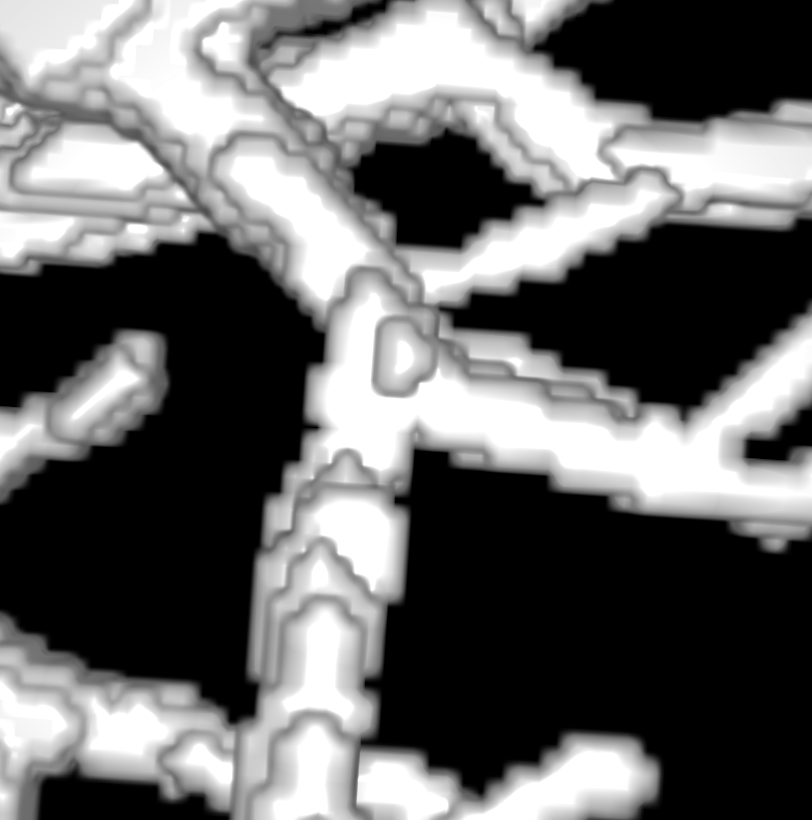
\includegraphics[clip = true, trim  = 0 50 0 80, width=19.0mm]{Images/Ircad_k_GT.png}
        \caption{Vérité terrain}
      \end{subfigure}
      \begin{subfigure}[t]{0.25\textwidth}
        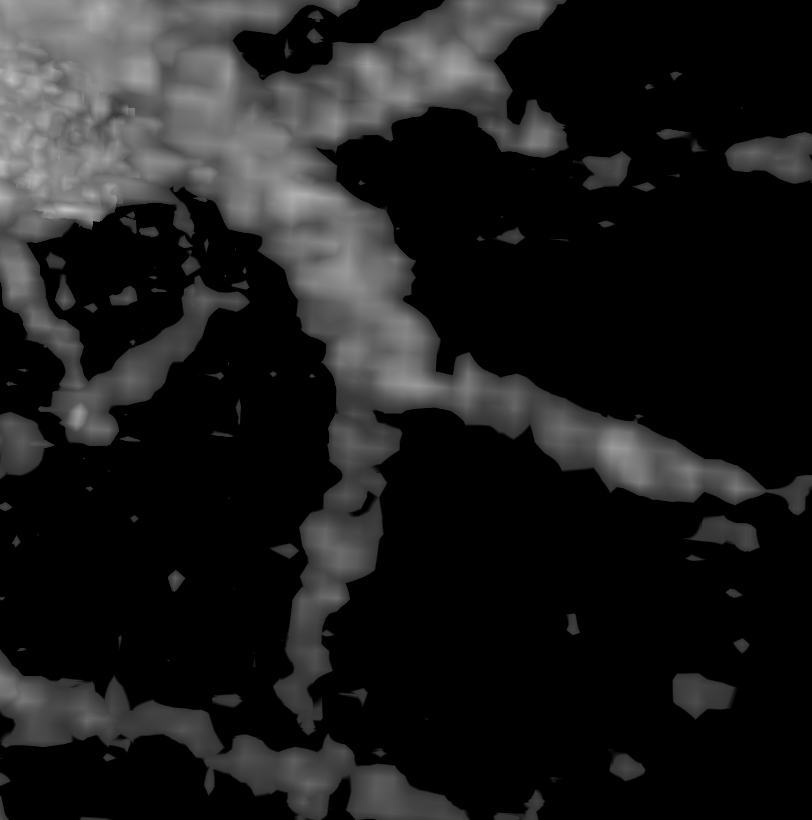
\includegraphics[clip = true, trim  = 0 50 0 80, width=19.0mm]{Images/Ircad_k_Baseline.png}
        \caption{Référence}
      \end{subfigure}
      \begin{subfigure}[t]{0.25\textwidth}
        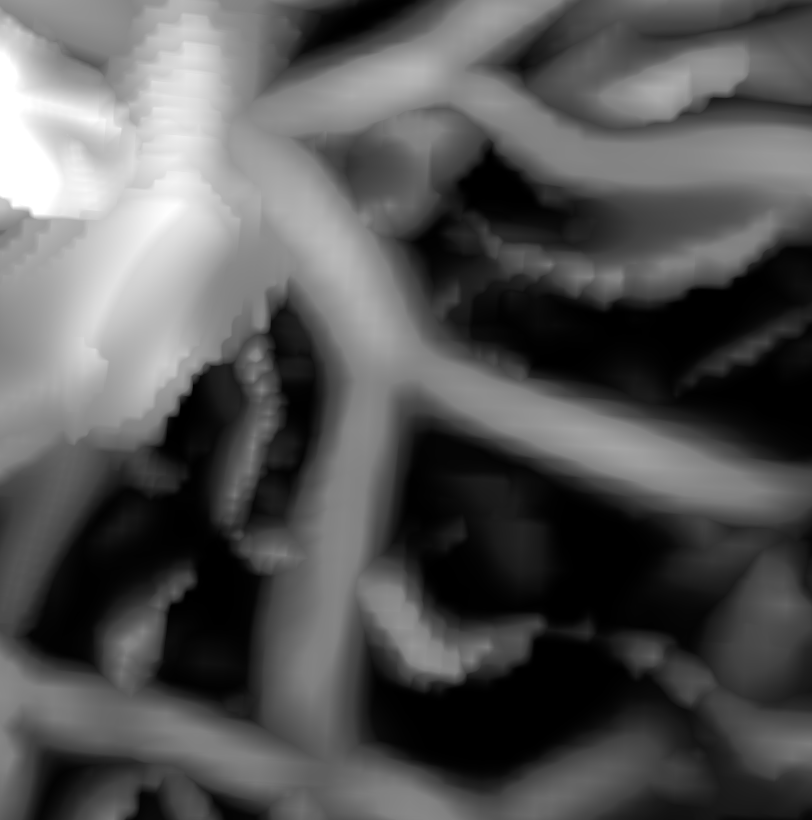
\includegraphics[clip = true, trim  = 0 50 0 80, width=19.0mm]{Images/Ircad_k_Frangi.png}
        \caption{Frangi}
      \end{subfigure}
      \begin{subfigure}[t]{0.25\textwidth}
        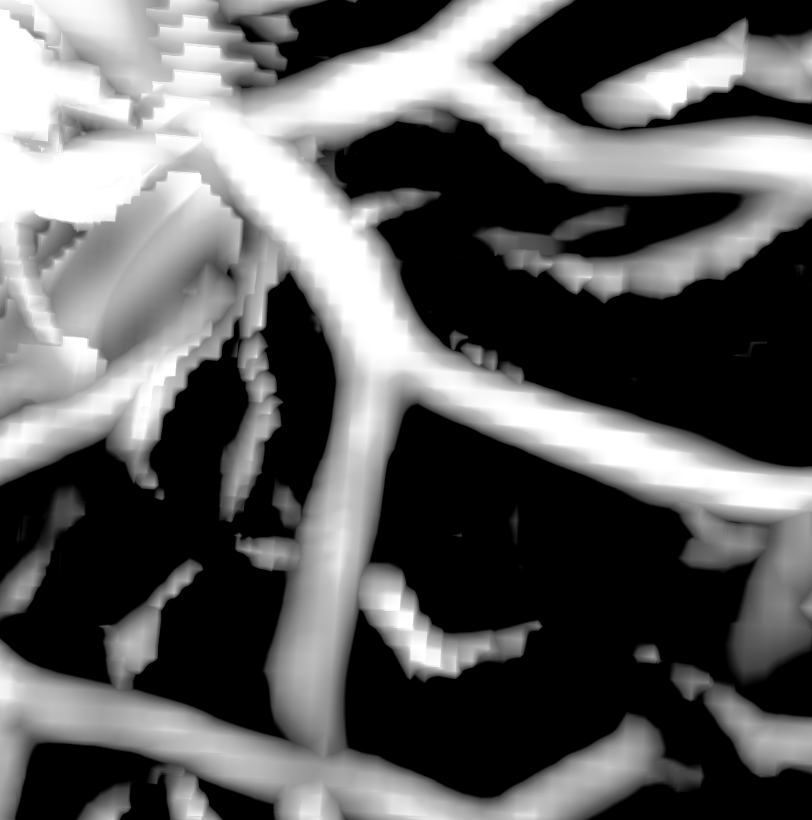
\includegraphics[clip = true, trim  = 0 50 0 80, width=19.0mm]{Images/Ircad_k_Jerman.png}
        \caption{Jerman}
      \end{subfigure}
      \begin{subfigure}[t]{0.25\textwidth}
        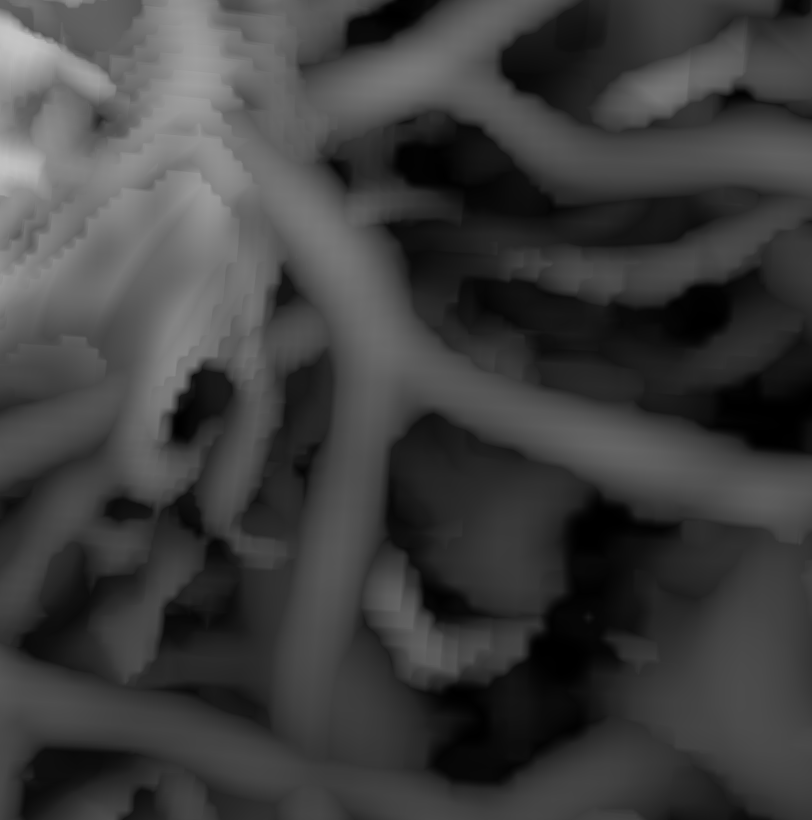
\includegraphics[clip = true, trim  = 0 50 0 80, width=19.0mm]{Images/Ircad_k_OOF_GM.png}
        \caption{OOF}
      \end{subfigure}
      \begin{subfigure}[t]{0.25\textwidth}
        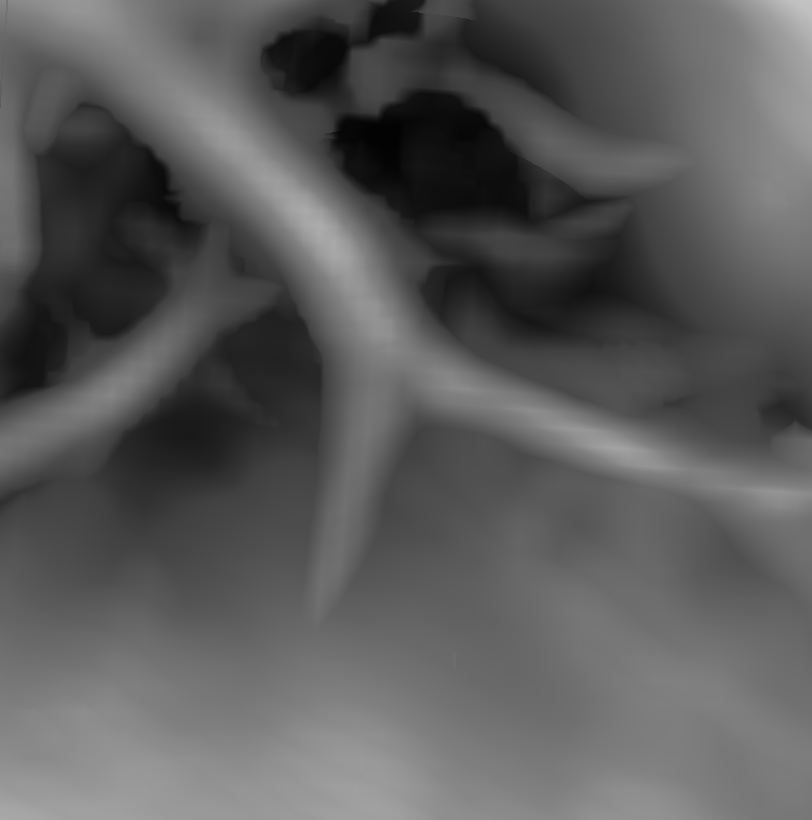
\includegraphics[clip = true, trim  = 0 50 0 80, width=19.0mm]{Images/Ircad_k_Meijering.png}
        \caption{Meijering}
      \end{subfigure}
      \begin{subfigure}[t]{0.25\textwidth}
        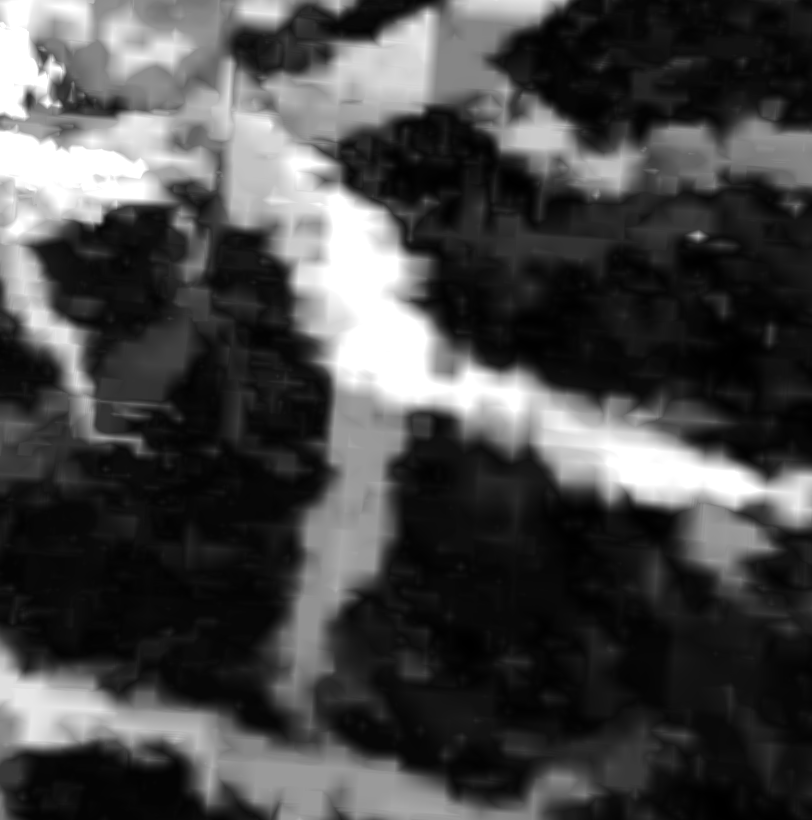
\includegraphics[clip = true, trim  = 0 50 0 80, width=19.0mm]{Images/Ircad_k_RORPO.png}
        \caption{RORPO}
      \end{subfigure}
      \begin{subfigure}[t]{0.25\textwidth}
        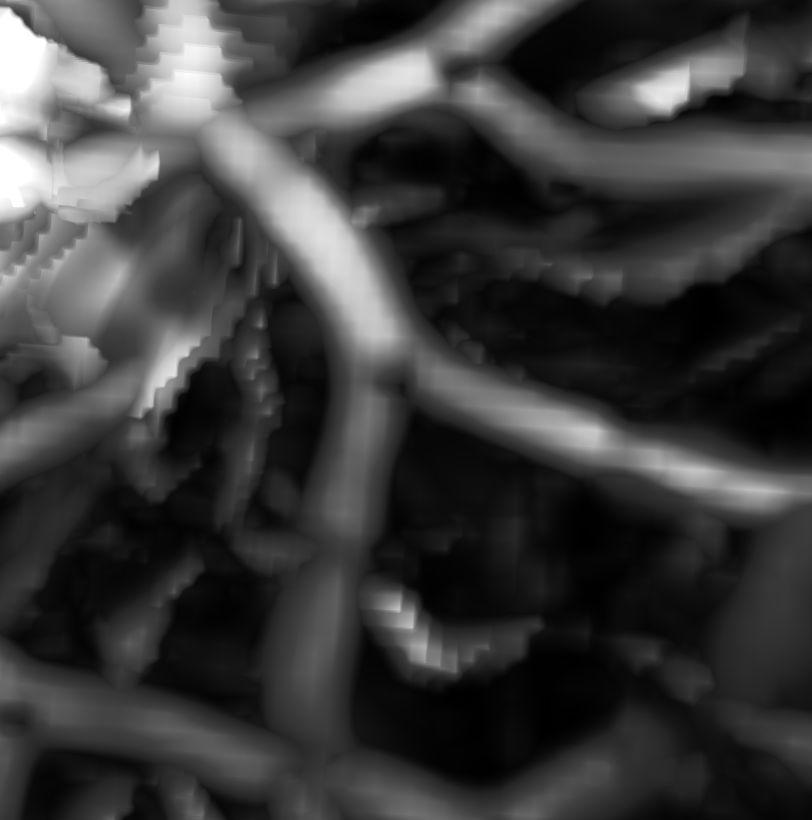
\includegraphics[clip = true, trim  = 0 50 0 80, width=19.0mm]{Images/Ircad_k_Sato.png}
        \caption{Sato}
      \end{subfigure}
      \begin{subfigure}[t]{0.25\textwidth}
        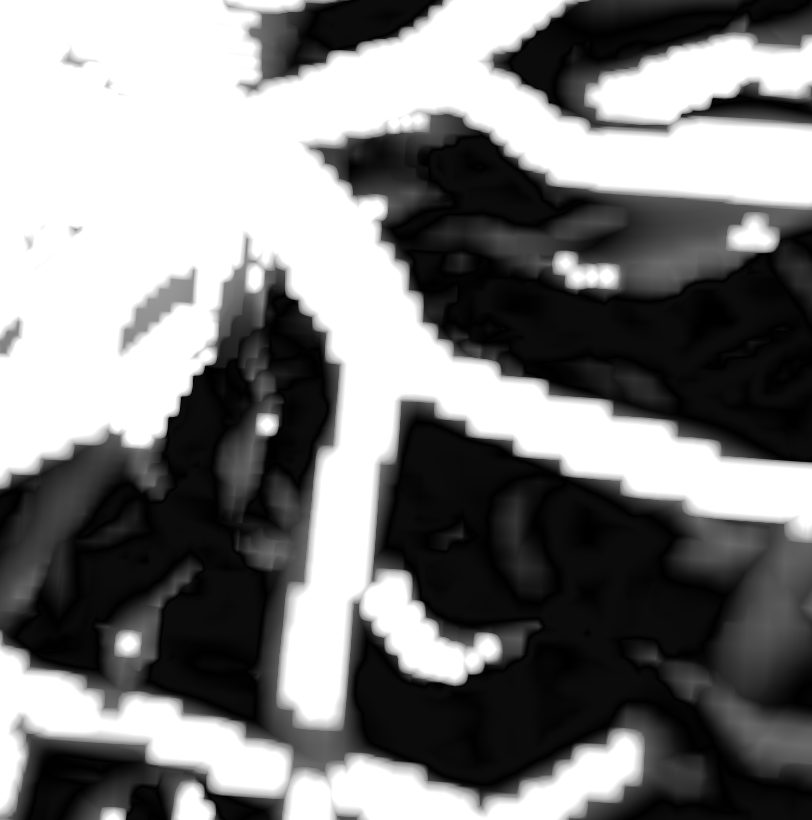
\includegraphics[clip = true, trim  = 0 50 0 80, width=19.0mm]{Images/Ircad_k_Zhang.png}
        \caption{Zhang}
      \end{subfigure}

      \caption{MIP des filtres avec les meilleurs paramètres sur une bifurcation pour le jeu de données VascuSynth avec $\sigma=2$ (première ligne) et le dataset de l'Ircad (deuxième ligne). La référence est l'image originale masquée et seuillée de manière optimale par rapport au MCC.
      }
      \label{fig:bifurcation_Ircad}
  \end{figure}
  
  \begin{figure}[H]
    \centering
    \begin{subfigure}[t]{0.25\textwidth}
      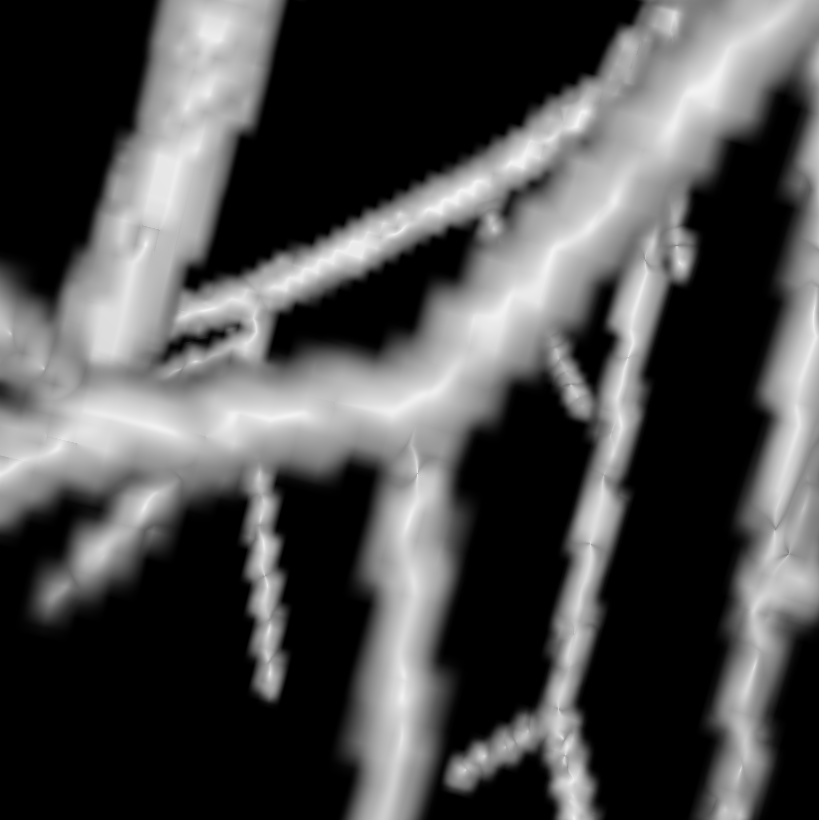
\includegraphics[clip = true, trim  =  170 230 150 240, width=19.0mm]{Images/Vascu_2_k_GT.png}
      \caption{Vérité terrain}
    \end{subfigure}
    \begin{subfigure}[t]{0.25\textwidth}
      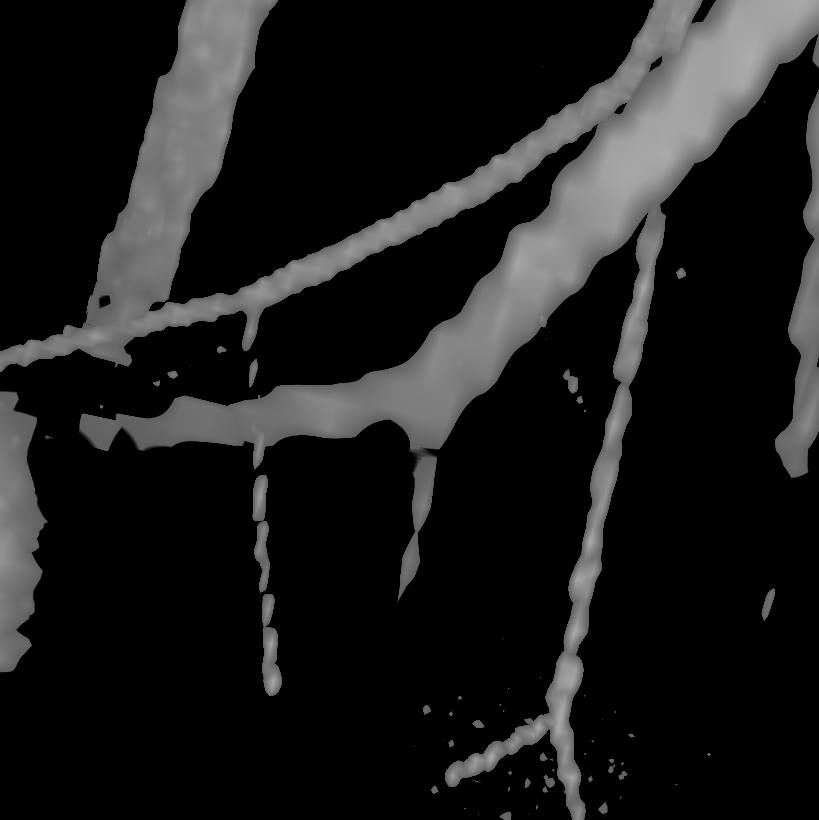
\includegraphics[clip = true, trim  =  170 230 150 240, width=19.0mm]{Images/Vascu_2_k_Baseline.png}
      \caption{Référence}
    \end{subfigure}
    \begin{subfigure}[t]{0.25\textwidth}
      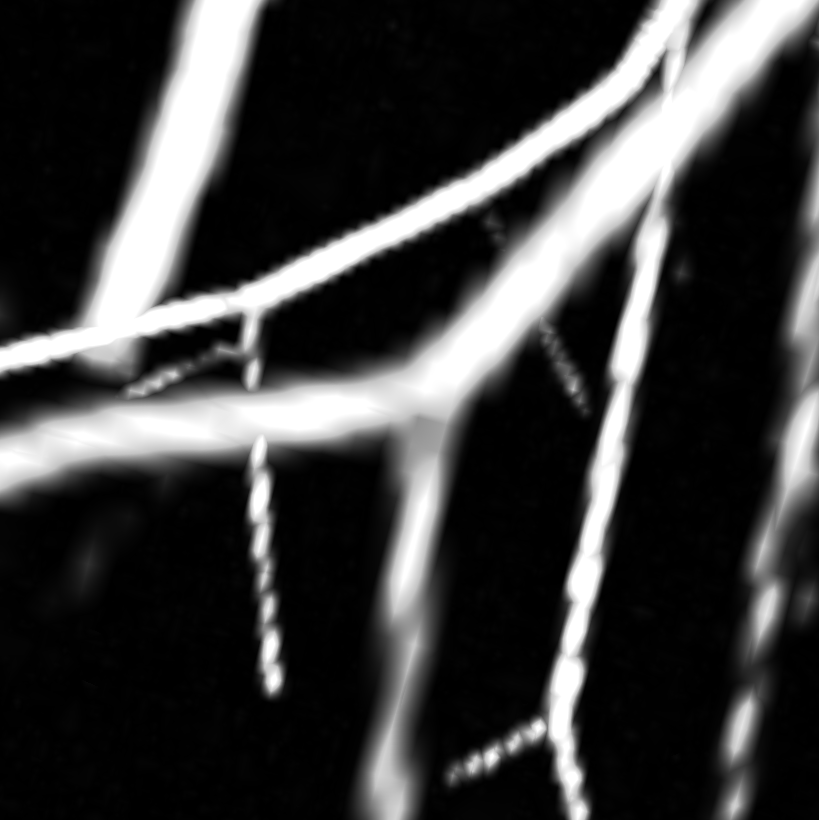
\includegraphics[clip = true, trim  =  170 230 150 240, width=19.0mm]{Images/Vascu_2_k_Frangi.png}
      \caption{Frangi}
    \end{subfigure}
    \begin{subfigure}[t]{0.25\textwidth}
      \includegraphics[clip = true, trim  =  170 230 150 240, width=19.0mm]{Images/Vascu_2_k_Jerman.png}
      \caption{Jerman}
    \end{subfigure}
    \begin{subfigure}[t]{0.25\textwidth}
      \includegraphics[clip = true, trim  =  170 230 150 240, width=19.0mm]{Images/Vascu_2_k_OOF_GM.png}
      \caption{OOF}
    \end{subfigure}
    \begin{subfigure}[t]{0.25\textwidth}
      \includegraphics[clip = true,trim  =  170 230 150 240, width=19.0mm]{Images/Vascu_2_k_Meijering.png}
      \caption{Meijering}
    \end{subfigure}
    \begin{subfigure}[t]{0.25\textwidth}
      \includegraphics[clip = true, trim  =  170 230 150 240, width=19.0mm]{Images/Vascu_2_k_RORPO.png}
      \caption{RORPO}
    \end{subfigure}
    \begin{subfigure}[t]{0.25\textwidth}
      \includegraphics[clip = true, trim  =  170 230 150 240, width=19.0mm]{Images/Vascu_2_k_Sato.png}
      \caption{Sato}
    \end{subfigure}
    \begin{subfigure}[t]{0.25\textwidth}
      \includegraphics[clip = true, trim  =  170 230 150 240, width=19.0mm]{Images/Vascu_2_k_Zhang.png}
      \caption{Zhang}
    \end{subfigure}

        \caption{MIP des filtres avec les meilleurs paramètres sur une bifurcation pour le jeu de données VascuSynth avec $\sigma=2$. La référence est l'image originale masquée et seuillée de manière optimale par rapport au MCC.
        }
      \label{fig:bifurcation_vascu}
  \end{figure}


\begin{figure}[!ht]
  \centering
      \begin{subfigure}[t]{0.25\textwidth}
          \begin{tikzpicture}
              \node[anchor=south west,inner sep=0] (image) at (0,0) {\includegraphics[clip = true, trim = 40 100 40 70, width=26.0mm]{Images/Bullitt_k_GT.png}};
              \begin{scope}[x={(image.south east)},y={(image.north west)}]
                  \draw[green,thick] (0.33,0.60) rectangle (0.43,0.75);
                  \draw[red,thick] (0.50,0.10) rectangle (0.65,0.35);
              \end{scope}
          \end{tikzpicture}
          \caption{Vérité terrain}
        \end{subfigure}
      \begin{subfigure}[t]{0.25\textwidth}
          \begin{tikzpicture}
              \node[anchor=south west,inner sep=0] (image) at (0,0) {\includegraphics[clip = true, trim = 40 100 40 70,  width=26.0mm]{Images/Bullitt_k_Baseline.png}};
              \begin{scope}[x={(image.south east)},y={(image.north west)}]
                  \draw[green,thick] (0.33,0.60) rectangle (0.43,0.75);
                  \draw[red,thick] (0.50,0.10) rectangle (0.65,0.35);
              \end{scope}
          \end{tikzpicture}
          \caption{Référence}
        \end{subfigure}
      \begin{subfigure}[t]{0.25\textwidth}
          \begin{tikzpicture}
                  \node[anchor=south west,inner sep=0] (image) at (0,0) {\includegraphics[clip = true, trim = 40 100 40 70,  width=26.0mm]{Images/Bullitt_k_Frangi.png}};
              \begin{scope}[x={(image.south east)},y={(image.north west)}]
                  \draw[green,thick] (0.33,0.60) rectangle (0.43,0.75);
                  \draw[red,thick] (0.50,0.10) rectangle (0.65,0.35);
              \end{scope}
          \end{tikzpicture}
          \caption{Frangi}
        \end{subfigure}
      \begin{subfigure}[t]{0.25\textwidth}
          \begin{tikzpicture}
                  \node[anchor=south west,inner sep=0] (image) at (0,0) {\includegraphics[clip = true, trim = 40 100 40 70,  width=26.0mm]{Images/Bullitt_k_Jerman.png}};
              \begin{scope}[x={(image.south east)},y={(image.north west)}]
                  \draw[green,thick] (0.33,0.60) rectangle (0.43,0.75);
                  \draw[red,thick] (0.50,0.10) rectangle (0.65,0.35);
              \end{scope}
          \end{tikzpicture}
          \caption{Jerman}
        \end{subfigure}

      \begin{subfigure}[t]{0.25\textwidth}
          \begin{tikzpicture}
                  \node[anchor=south west,inner sep=0] (image) at (0,0) {\includegraphics[clip = true, trim = 40 100 40 70,  width=26.0mm]{Images/Bullitt_k_OOF_GM.png}};
              \begin{scope}[x={(image.south east)},y={(image.north west)}]
                  \draw[green,thick] (0.33,0.60) rectangle (0.43,0.75);
                  \draw[red,thick] (0.50,0.10) rectangle (0.65,0.35);
              \end{scope}
          \end{tikzpicture}
          \caption{OOF}
        \end{subfigure}
      \begin{subfigure}[t]{0.25\textwidth}
          \begin{tikzpicture}
                  \node[anchor=south west,inner sep=0] (image) at (0,0) {\includegraphics[clip = true, trim = 40 100 40 70,  width=26.0mm]{Images/Bullitt_k_Meijering.png}};
              \begin{scope}[x={(image.south east)},y={(image.north west)}]
                  \draw[green,thick] (0.33,0.60) rectangle (0.43,0.75);
                  \draw[red,thick] (0.50,0.10) rectangle (0.65,0.35);
              \end{scope}
          \end{tikzpicture}
          \caption{Meijering}
      \end{subfigure}
      \begin{subfigure}[t]{0.25\textwidth}
          \begin{tikzpicture}
                  \node[anchor=south west,inner sep=0] (image) at (0,0) {\includegraphics[clip = true, trim = 40 100 40 70,  width=26.0mm]{Images/Bullitt_k_RORPO.png}};
              \begin{scope}[x={(image.south east)},y={(image.north west)}]
                  \draw[green,thick] (0.33,0.60) rectangle (0.43,0.75);
                  \draw[red,thick] (0.50,0.10) rectangle (0.65,0.35);
              \end{scope}
          \end{tikzpicture}
          \caption{RORPO}
        \end{subfigure}
      \begin{subfigure}[t]{0.25\textwidth}
          \begin{tikzpicture}
                  \node[anchor=south west,inner sep=0] (image) at (0,0) {\includegraphics[clip = true, trim = 40 100 40 70,  width=26.0mm]{Images/Bullitt_k_Sato.png}};
              \begin{scope}[x={(image.south east)},y={(image.north west)}]
                  \draw[green,thick] (0.33,0.60) rectangle (0.43,0.75);
                  \draw[red,thick] (0.50,0.10) rectangle (0.65,0.35);
              \end{scope}
          \end{tikzpicture}
          \caption{Sato}
        \end{subfigure}
      \begin{subfigure}[t]{0.25\textwidth}
          \begin{tikzpicture}
                  \node[anchor=south west,inner sep=0] (image) at (0,0) {\includegraphics[clip = true, trim = 40 100 40 70,  width=26.0mm]{Images/Bullitt_k_Zhang.png}};
              \begin{scope}[x={(image.south east)},y={(image.north west)}]
                  \draw[green,thick] (0.33,0.60) rectangle (0.43,0.75);
                  \draw[red,thick] (0.50,0.10) rectangle (0.65,0.35);
              \end{scope}
          \end{tikzpicture}
          \caption{Zhang}
        \end{subfigure}
      
        \caption{
        MIP des vaisseaux au centre du cerveau pour le jeu de données Bullitt. Ces vaisseaux sont situés sur le même plan, illustrant ainsi les vaisseaux proches (rouge) et les bifurcations (vert).}
      \label{fig:bifurcation_Bullitt}
\end{figure}

Le filtrage des bifurcations est présenté visuellement dans les figures \ref{fig:bifurcation_Ircad} et \ref{fig:bifurcation_vascu} pour VascuSynth et l'Ircad, tandis que les bifurcations et les vaisseaux adjacents de Bullitt sont présentés dans les figures \ref{fig:bifurcation_Bullitt}.

Qualitativement, nous observons que les filtres de Frangi et Sato montrent une perte de signal au centre des bifurcations pour l'Ircad et Bullitt et sur les côtés de la bifurcation pour VascuSynth. Cette perte de signal n'a pas été observée pour les autres filtres. Le déplacement de la perte de signal s'éloignant des bords pour VascunSynth peuvent s'expliquer par une géométrie particulière pour ce jeu de données. En effet, les nouvelles branches partant d'un vaisseau principal plus gros ont une épaisseur plus réduite, translatant ainsi le centre de la bifurcation de l'intersection des deux vaisseaux à la base du plus petit. Concernant les vaisseaux adjacents, certains filtres montrent une tendance à fusionner les vaisseaux très proches. Ces filtres sont Jerman, Meijering et Zhang. Les autres filtres tels que Frangi, Sato, OOF et RORPO semblent plus robustes à cet effet. En particulier, cette robustesse est assurée par la propriété anti-extensive du filtre.

\section{Discussion}

Basé sur ces expériences, on peut formuler quelques recommandations en fonction du masque de région d'intérêt.

Nous avons observé que les performances de Meijering sont faibles dans les jeux de données réels, puisque le filtre rehausse fortement le bruit. Ce comportement est consistant avec le fait que Meijering est un filtre dédié au rehaussement dans des images très faiblement contrastés pour des applications de tracking. Il faut toutefois noté que Meijering présentait de bons résultats sur les données synthétiques de VascuSynth. Meijering peut donc être appliqué pour plusieurs contextes :

\begin{itemize}
  \item Les images sont faiblement contrastées et présentent une géométrie des vaisseaux relativement droite sans variations de diamètres.
  \item L'utilisateur choisit d'appliquer une segmentation basée sur une stratégie de tracking et/ou applique une stratégie de post traitement capable d'identifier les faux positifs.
\end{itemize}

OOF, couplé avec la mesure de tubularité de la moyenne géométrique, présente des résultats relativement faibles sur nos jeux de données, ce qui peut s'expliquer par deux éléments : (1) Le choix de la mesure dont le pouvoir de discrimination entre les plateaux et les structures tubulaires est faible; et (2) OOF est basé sur l'hypothèse de tranches des vaisseaux à géométrie circulaire, ce qui en pratique n'est pas toujours le cas, en particulier pour l'Ircad. Il faut aussi noter que OOF est une cadre d'espace d'échelles et que différentes mesures de tubularités peuvent être utilisées en fonction de l'application d'intérêt. OOF est un bon choix dans les cas suivants : 

\begin{itemize}
  \item Les vaisseaux présentent des tranches circulaires.
  \item Les réseaux vasculaires présentes un nombre important de vaisseaux adjacents.
\end{itemize}

Sato et Frangi présentent tous les deux de bonnes performances dans notre banc de test. Ces deux filtres proposent un bon compromis entre sensibilité et spécificité, mais produisent la plupart du temps une perte de signal au niveau des bifurcations. Nous recommandons Frangi dans les cas suivants :

\begin{itemize}
  \item Les vaisseaux dans les images sont de tailles supérieures à quelques voxels.
  \item L'utilisateur a besoin d'un contrôle efficace sur le niveau de bruit à filtrer, au prix de la perte des petits vaisseaux.
\end{itemize}

Sato est recommandé dans les cas suivants :

\begin{itemize}
  \item Les images présentent peu de bruit.
  \item Les vaisseaux ont des tranches circulaires.
  \item Les réseaux vasculaires présentent des vaisseaux adjacents.
\end{itemize}

Jerman présente de bonnes performances avec une sensibilité importante et dessine des contours de vaisseaux nets. Cependant, le filtre a tendance à être plus sensible au bruit que les filtres hessiens classiques (i.e. Frangi et Sato) et partage la même tendance à sur estimer le volume des vaisseaux. Nous recommandons le Filtre de Jerman dans les cas suivants : 

\begin{itemize}
\item Les images avec de petits vaisseaux
\item Les images avec un faible niveau de bruit.
\end{itemize} 

Zhang est une version modifiée de Jerman, créé pour être moins sensible aux bords et aux artefacts de bordure. Malheureusement la méthode est limitée à des organes spécifiques (ici le  foie). Bien que la méthode propose des résultats intéressants, celle-ci requiert une connaissance a priori de la distribution des intensités des structures de l'image seulement disponible pour certaines applications. Zhang est un bon filtre dans les cas suivants :

\begin{itemize}
\item Les applications où des masques sont disponibles.
\item Un contraste constant des vaisseaux dans l'image.
\end{itemize}

RORPO obtient la première place dans les deux jeux de données réels, mais produit des résultats faibles pour le jeu de données synthétique VascuSynth. Le filtre différencie de manière efficace les bords des organes des structures tubulaire et ne surestime jamais la taille des vaisseaux. Cependant RORPO favorise la spécificité par rapport à la sensibilité et de ce fait présente un plus grand nombre de faux négatifs que les autres méthodes. RORPO est un bon choix pour les applications suivantes :

\begin{itemize}
  \item Les applications nécessitant la détection des contours précis des vaisseaux.
  \item Les applications avec une faible tolérance aux faux négatifs ( e.g. quand le pot-processing n'est pas disponible). 
\end{itemize}

\subsection{Influence des paramètres}

Une des questions que nous nous sommes posés était de connaitre l'influence des paramètres des filtres. D'identifier quels paramètres jouent un rôle significatif et de comprendre les choix des paramètres par défauts proposés par les auteurs lorsque c'est le cas. Les paramètres optimaux à la suite de nos expériences sont résumés dans la Tab. \ref{tab:optimal_parameters}.

\begin{table}[!ht]
 
  \begin{center}
  \caption{Paramètres optimaux des 7 filtres dans les 3 jeux de données}
      \begin{tabular}{llrrrrr}
                          \hline
             & Parameter  & Ircad       &  \multicolumn{3}{c}{VascuSynth}            &  Bullitt\\
             & Parameter  &         & $\sigma = 2$  & $\sigma = 4$ & $\sigma = 6$ &       \\
                         \hline
      Frangi &  $\alpha$  & $1$         & $0.2$     & $0.2$        & $0.2$           & $1.0$   \\
      ---    &  $\beta$   & $1$         & $0.6$     & $0.4$       & $0.4$           & $0.4$   \\
      ---    &  $C$       & $30$        & $30$       & $30$         & $30$            & $30$    \\
      Jerman & $\tau$     & $0.1$       & $0.2$     & $0.2$       & $0.3$          & $0.2$  \\
      OOF &  $\sigma$     & $1$         & $0.1$      & $0.1$        & $0.1$           & $0.1$   \\
      RORPO  & Scale min  & $70$        & $50$       & $50$         & $40$            & $20$    \\
      ---    &Factor      & $1.3$       & $1.1$     & $1.2$       & $1.4$          & $1.3$  \\
      ---    &  nbScales  & $4$         & $3$        & $2$          & $2$             & $4$     \\
      Sato   & $\alpha_1$ & $0.3$       & $0.3$      & $0.3$        & $0.5$          & $0.7$   \\
      Sato   & $\alpha_2$ & $1.6$       & $2$      & $1$        & $2$           & $1.0$   \\
      Zhang  & $\tau$     & $0.3$       & $0.4$     & $0.8$       & $0.9$          & $0.1$  \\
          \hline
      \end{tabular}
  \label{tab:optimal_parameters}
  \end{center}
\end{table}


\subsection{Paramètres d'échelles}

Le choix des paramètres d'échelles sont déterminants pour l'ensemble des filtres. Lorsque la technique de rehaussement est efficace, les variations entre une échelle non optimisée et une échelle optimisée sont très importante. Entre le moins bon jeu de paramètres et le meilleur jeu de paramètre (étape 1 de l'optimisation), des variations de MCC entre $0.23$ et $0.30$ ont été observées pour les filtres Hessien. Pour RORPO, dont le paramétrage repose exclusivement sur l'échelle des chemins composés par les élements structurants, une variation moyenne de $0.18$ du MCC a été observée. OOF montre le delta le plus faible, avec des variations de MCC moyennes de $0.07$. Une hypothèse, est que la majeure partie des vaisseaux soient capturés dans une seule échelle, limitant l'impact de l'optimisation.

\subsection{Paramètres intrinsèques}

Pour l'optimisation des paramètres intrinsèque, Frangi est le filtre montrant le plus de variations de performances avec un MCC variant de $0.30$ entre le pire jeu de paramètre et le meilleur. On pouvait s'y attendre, puisque les paramètres composants la mesure de tubularité de Frangi touchent à des concepts très différents. De plus, l'optimisation montre que des combinaisons de jeux de paramètres assez éloignés produisent des résultats assez similaires en terme de MCC. Par exemple les paramètres $\alpha=0.40,\beta=1,C=30$, $\alpha=0.60,\beta=1.00,C=30$ et $\alpha=1,\beta=0.40,C=30$ produisent des MCC moyens sur l'Ircad de $0.342$, $0.351$ et $0.3515$. On obtient donc des résultats quantitatifs similaires avec des valeurs de suppression de blobs et de plateaux assez différents.

On peut visualiser de quelle manière les paramètres impactent le rehaussement en simulant une grille de valeurs propres négatives (Fig. \ref{exemple_geometry}). Chaque axe représente l'évolution d'une valeur propre de 0 à une borne négative $B$ avec un pas $P$. Pour chaque triplet ($\lambda_1,\lambda_2,\lambda_3$) on peut ainsi calculer le rehaussement en connaissant en amont la géométrie. Sur cette grille, la diagonale de 0 à ($B_1,B_2,B_3$) correspond aux blobs, 3 points correspondent à des structures tubulaires parfaites, le reste des points formes des structures en plateaux.

\begin{figure}[H]
  \centering
  \includegraphics[height=5cm]{Images/eigen_meaning.png}
  \label{fig:exemple_geometry}
  \caption{Correspondance entre géométrie et valeurs propre. Les 3 structures tubulaires parfaites sont en bleu. La diagonale rouge représente les blobs. Les plateaux sont représentés par des structures vertes. Le reste sont des interpolations de ces trois configurations}
\end{figure}


En moyenne, une variation de MCC de $0.2$ a été observé entre les paramètres par défaut proposés par Frangi et les paramètres optimisés. D'un point de vue géométrique, les paramètres par défaut ($\alpha=0.5,\beta=0.5$) correspondent à un modèle de tubularité modéré. Les paramètres optimisés correspondent à un modèle plus relâché qui accepte des structures plus structures planaires et sphériques (Fig. \ref{fig:exemple_geometry_frangi}). Le filtre de Frangi présente le méchanisme d'atténuation de bruit le plus paramétrable et le plus efficace.

\begin{figure}[H]

  \begin{subfigure}[t]{0.45\textwidth}
    \includegraphics[height=5cm]{Images/Bullitt_Frangi_BP.png}
    \caption{Bullitt}
  \end{subfigure}
  \begin{subfigure}[t]{0.45\textwidth}
    \includegraphics[height=5cm]{Images/Ircad_Frangi_BP.png}
    \caption{Ircad}
  \end{subfigure}
  \begin{subfigure}[t]{0.45\textwidth}
    \includegraphics[height=5cm]{Images/Vascu_2_Frangi_BP.png}
    \caption{Vascu $\sigma=2$}
  \end{subfigure}
  \begin{subfigure}[t]{0.45\textwidth}
    \includegraphics[height=5cm]{Images/Frangi_default_P.png}
    \caption{Paramètres de Frangi}
  \end{subfigure}
  \label{fig:exemple_geometry_frangi}
  \caption{Visualisation des différents paramètres optimaux obtenus pour Frangi(Tab. \ref{tab:optimal_parameters}). Les paramètres par défauts sont présentés à titre indicatif.}
\end{figure}


Les filtres de Jerman et Zhang montrent de très faible variation de MCC autour de $0.04$. Ceci est très probablement causé par le seuillage automatique qui compense l'effet du paramètre Tau, dont le rôle est de contrôler l'homogénéité de la réponse du filtre. En terme de géométrie, les filtres de Jerman et Zhang sont les filtres qui relâchent le plus les contraintes sur le modèle de tubularité avec un rehaussement fort aussi bien pour les structures tubulaires que les blob/bifurcations. La contrainte est aussi beaucoup plus relâchée sur tubes qui présenteraient des structures plus planaires (Fig. \cite{exemple_geometry_jerman}).

\begin{figure}[H]

  \begin{subfigure}[t]{0.45\textwidth}
    \includegraphics[height=5cm]{Images/Bullitt_Jerman_BP.png}
    \caption{Bullitt}
  \end{subfigure}
  \begin{subfigure}[t]{0.45\textwidth}
    \includegraphics[height=5cm]{Images/Ircad_Jerman_BP.png}
    \caption{Ircad}
  \end{subfigure}

  \label{fig:exemple_geometry_jerman}
  \caption{Paramètres optimaux pour Bullitt et l'Ircad pour le filtre de Jerman. Le rehaussement est clairement plus homogène et permissif qu'un filtre comme Frangi ou Sato.}
\end{figure}

Le filtre de Sato présente très peu de variations par jeux de paramètres avec une variation maximale moyenne de MCC de 0.02. Les paramètres par défaut proposés par Sato, sont donc très proches des paramètres optimaux trouvés. D'un point de vue géométrie, Sato propose une mesure assez stricte par rapport à la définition de la tubularité, avec une réponse forte pour les tubes. En particulier, le paramètre $\alpha_1$ contrôle la relaxe du modèle envers les blobs/bifurcations (Fig. \ref{fig:exemple_geometry_Sato}).


\begin{figure}[H]

  \begin{subfigure}[t]{0.45\textwidth}
    \includegraphics[height=5cm]{Images/Bullitt_Sato_BP.png}
    \caption{Bullitt}
  \end{subfigure}
  \begin{subfigure}[t]{0.45\textwidth}
    \includegraphics[height=5cm]{Images/Ircad_Sato_BP.png}
    \caption{Ircad}
  \end{subfigure}

  \label{fig:exemple_geometry_Sato}
  \caption{Paramètres optimaux pour Bullitt et l'Ircad pour le filtre de Sato. Le rehaussement est plus strict en limitant le rehaussement à des variations plus faibles de la géométrie.}
\end{figure}

Il faut aussi noter que la plupart des paramètres optimaux des filtres ne sont pas choisis en fonction de leur capacité à produire une réponse forte en valeur absolue, mais à différencier les structures en valeurs relatives. Il est très possible que l'ajout de cette contrainte modifie les résultats, par exemple pour le cas du manque de signal des bifurcations.
Dans un cas réel, il est difficile de trouver le seuil optimal puisque la vérité terrain n'est pas disponible. Dans un contexte avec un seuil de décision fixe, les paramètres optimaux changent très probablement. De plus, il devient important d'obtenir le rehaussement en valeur absolue le plus haut. On pourrait probablement vérifier cette hypothèse en optimisant les paramètres afin qu'ils maximisent le PSNR.

En effet, on peut noter que dans notre expérience, la plupart des volumes de résultats nécessitent un ajustement de la fenêtre de représentation des niveaux de gris à la visualisation, car les valeurs absolues de rehaussement sont souvent basses.

\section{Bilan}

Dans ce chapitre, nous avons analysé 7 filtres de rehaussements. Cette analyse repose à la fois sur les comparaisons des performances entre les filtres et la comparaison des performances de différents jeux de paramètres. 

Nous avons exposé des différences notables entre les filtres dans leur capacité à rehausser le réseau vasculaire dans son ensemble, mais aussi à rehausser des parties spécifiques du réseau, tel que les vaisseaux fins. Nous avons aussi montré que leur performance peut varier significativement en présence de bruit. De plus, nous avons exposé les différentes faiblesses des filtres comme les bordures des organes.

Nous avons aussi démontré l'importance de la paramétrisation de l'espace d'échelles des filtres qui influe de manière significative sur la capacité des filtres à capturer l'ensemble des tailles de vaisseaux présents.

Pour les paramètres intrinsèques des filtres, nous avons montré qu'ils jouaient, eux aussi, un rôle dans les performances des filtres. En effet, une mauvaise paramétrisation des paramètres peut faire chuter les performances des filtres de manière importante. Cette chute de performance est d'autant plus marquée dans des situations réelles lorsque choisir un seuil optimal après le rehaussement est particulièrement complexe.

En tant que filtre sans paramètres intrinsèques, Meijering est le plus simple des filtres à paramétrer. RORPO et OOF sont aussi simple à paramétrer puisque RORPO n'a qu'un seul paramètre intrinsèque binaire (le paramètre de dilatation) et OOF dépend seulement d'un paramètre de lissage $\sigma$. Jerman et Zhang ont, eux aussi, un seul paramètre intrinsèque à régler, $\tau$, qui contrôle à la fois la netteté des bordures des vaisseaux et l'homogénéité du contraste. Dans la plupart des cas, le $\tau$ optimal est bas de manière à obtenir une réponse homogène. 

Sato et Frangi sont les filtres les plus complexes à filtrer. Ils possèdent 2 et 3 paramètres intrinsèques qui sont difficiles à régler, car ils n'ont pas de sens intuitifs. Ces paramètres influencent directement la géométrie des structures et le résultat est donc sensible au changement de paramètres. Nous avons pu observer que les paramètres optimaux pour les deux filtres étaient choisis de manière à relaxer la contrainte de tubularité et rehausser les vaisseaux aux formes plus variés. Cependant, le gain de performances n'est pas significatif par rapport aux paramètres par défaut recommandés par les auteurs.

Le temps de calcul moyen pour chaque filtre sur trois volumes de chaque jeu de données est présenté dans la table \ref{tab:Computation time benchmark}. Tous les filtres Hessiens sont relativement équivalents (environ 1min par volume), excepté pour Zhang puisque l'étape de K-moyenne prend plus de temps à calculer.

\begin{table}
  \centering
  \caption{Computational cost the the seven filters (CPU time in seconds) mean over 3 volumes of each dataset.}
  \label{tab:Computation time benchmark}
  \begin{tabular}{lrrr}
  \hline
                     & Ircad      & Bullit  & VascuSynth \\
                     \hline
  Frangi    & ~~~~~~~~~$72$  & ~~~~~~~~~$47$   & ~~~~~~~~~$6$   \\
  Sato      & $67$  & $44$   & $5$   \\
  Meijering & $43$  & $36$   & $6$   \\
  OOF       & $231$  & $274$   & $17$   \\
  RORPO     & $1776$  & $1227$   & $160$   \\
  Jerman    & $39$  & $34$   & $6$   \\
  Zhang     & $106$  & $80$   & $10$  \\
  \hline
  \end{tabular}
  \end{table}

OOF et RORPO requiert beaucoup plus de puissance de calculs puisque leur complexité n'est pas linéaire avec la taille de l'image. Cependant, l'implémentation de RORPO est parallélisée pour réduire le temps de calcul. OOF peut-être implémenté sur GPU comme démontré par Law \cite{Law2009_efficient_implementation}.

Enfin, il est important que noter que le résultat de ces expériences dépend des jeux de données et des vérités terrains associées. Les jeux de données publiques sont rares et donc précieux, même si ceux-ci possèdent des limitations. En particulier, les vérités terrrains de l'Ircad manquent certains vaisseaux larges, ce qui peut influencer les métriques calculées. De plus le diamètre des vaisseaux est souvent sur estimé, ce qui ajoute un biais systématique (positif ou négatif en fonction des méthodes) dans les résultats quantitatifs. Le jeu de données VascuSynth étant synthétique, la géométrie des vaisseaux est plus simple que pour les vaisseaux réels, ce qui impact le résultat des filtres. De plus, le fond est bien plus simple que dans la plupart des images médicales qui contiennent d'autres structures et organes.



